\documentclass[a4paper]{article}
\usepackage{graphicx}
\usepackage{amsmath}
\usepackage{placeins}
\usepackage{multicol}
\usepackage{float}
\usepackage{tabularx}
\usepackage{textcomp}
\usepackage{caption}
\usepackage[margin=1.0in]{geometry}
\usepackage{natbib}
\usepackage{tabulary}
\usepackage{setspace}
\usepackage{epstopdf}
%\usepackage{subcaption}
\usepackage{braket}
%\usepackage[toc,page]{appendix}
\usepackage{cancel}
\usepackage{epstopdf}
\usepackage{subfig}
\usepackage{subfloat}
\usepackage{fancyhdr}
\usepackage{etoolbox} % Change definition of commands
%\usepackage{titling}

\font\myfont=cmr12 at 14pt
\font\smallmyfont=cmr12 at 12pt

%\makeatletter
%\patchcmd{\chapter}{\if@openright\cleardoublepage\else\clearpage\fi}{}{}{}
%\makeatother

\pagestyle{fancy}
\fancyhead[LO, RE]{}
\fancyfoot[C]{\thepage}
\renewcommand{\sectionmark}[1]{%
\markboth{\MakeUppercase{%
\thesection. \ #1}}{}}


\begin{document}

\thispagestyle{empty}
\begin{center}
\Large{Discounting low energy background scintillation signals in SBND}\\[2pc]

\large{Colton Hill, Andrzej Szelc, Diego Garcia-Gamez}\\[0.5pc]
\large{\today}\\[2pc]

SBND Internal Document\\
\end{center}
%\vspace{0.25cm}
%\begin{titlingpage}
    %\maketitle
\begin{abstract}
\noindent 

Scintillation light produced in large liquid argon detectors provide the opportunity to measure interesting low energy physics such as supernova neutrinos and nucleon decay. Several potential low energy backgrounds provide constant signals to the light detection system and can make detection of these signals impossible. In $^{39}$Ar decays the background occurs at a high rate compared to the arrival of supernova neutrinos. Using the fast optical simulation library, the backgrounds as well as supernova neutrinos can be quickly simulated throughout the SBND detector to compare the ability of the light system to detect these signals.  
%A hypothesised additional signal is also investigated, where ion recombination on the grounded cathode produces scintillation light. 
This document explores a simple set of cuts to remove the $^{39}$Ar backgrounds while preserving the supernova signal for three different light system configurations.

\end{abstract}
%\end{titlingpage}

\pagebreak
\tableofcontents
\pagebreak
%%-----------------------------------------------------------------------------------------------------------------------------------------------------
%%-----------------------------------------------------------------------------------------------------------------------------------------------------
%%%%%%%%%%%%%%%%%%%%%%%%%%%%%%%%%%%%%%%%%%%%%%%%%%%%%%%%%%
%%%%%%%%%%%%%%%%%%%%%%%%%%%%%%%%%%%%%%%%%%%%%%%%%%%%%%%%%%
\section{Scintillation from Low Energy Events in Liquid Argon Time Projection Chambers}

Liquid argon time projection chambers make use of argon's non-interactive nature by drifting charged particles through the detector to readout wires for distances as long as meters. Interactions inside the liquid argon volume produce an ion-electron pair, or result in an excitation of an argon atom. Upon recombination of the ion-electron pair or deexcitation of the argon atom scintillation light is produced. As a function of the electric field magnitude, the amount of charge reaching the wires and the amount of light produced are inversely correlated. With an increase in field strength, the amount of scintillation light decreases, as the recombination of electron-ion pairs decreases. The light signals are read out by PMTs generally located behind the wire planes. 

While SBND is being constructed primarily as a beam-line neutrino detector, and R\&D for future large liquid argon neutrino detectors (DUNE), the light detection system also provides a good opportunity to study low energy (sub 50 MeV) events. Galactic supernova neutrinos peak with an energy around 20 MeV, making the LDS the prime candidate to detect them, however the LDS is also being constantly bombarded by background from naturally occurring $^{39}$Ar. We show that the constant low energy background originating from  $^{39}$Ar 
%as well as hypothesised Ar ions recombining on the cathode 
 can be limited by setting thresholds on the PMTs as well as forming coincidences. The methods used to limit these backgrounds are explored further in the following sections. Sections \ref{sim_detail} and \ref{limiting_bkg} discuss the details of a simulation written to compare the $^{39}$Ar background and supernova neutrinos as well as conclusions drawn from the simulation regarding removing the background signal.

%This document will focus primarily on light signals expected to be detected in the PMT system of the SBND detector. The light system planned for the SBND detector involves an array of 60 PMTs, as well as possible wave length shifting foils to increase the light yield uniformity. Including a no-foil configuration, the two other configurations considered here are to include TPB-covered foils on the cathode, and on all walls of the detector. By including the TPB-covered foils, the light yield of the system increases without the addition of further PMTs, which increases the energy reconstruction capabilities of the detector. For more details regarding the SBND light system, please see DocDB 1155. 

\section{$^{39}$Ar and Supernova Neutrinos}

$^{39}$Ar beta-decays with Q = 0.565 MeV and is created by cosmic ray interactions. The resulting activity of 1 Bq/kg means detectors like SBND will have a constant supply of low energy electrons being emitted throughout the detector. The emitted electrons ionise the liquid argon and produce scintillation photons, where the number produced is a function of the scintillation yield of the medium and the energy of the electron. Figure \ref{ar_spectrum} shows the beta-decay energy spectrum for $^{39}$Ar, where the most common decay energy is around 200 keV. Given SBND's expected electric field magnitude of 500 V/cm, the scintillation yield is taken to be 24,000 $\gamma$/MeV for low mass particles, meaning an average decay produces roughly 4,800 photons. The constant background of scintillation light from the $^{39}$Ar decays could make it impossible to distinguish between background generated photons and other low energy signals seen in the detector, such as supernova neutrinos.

\begin{figure}[H]
\center
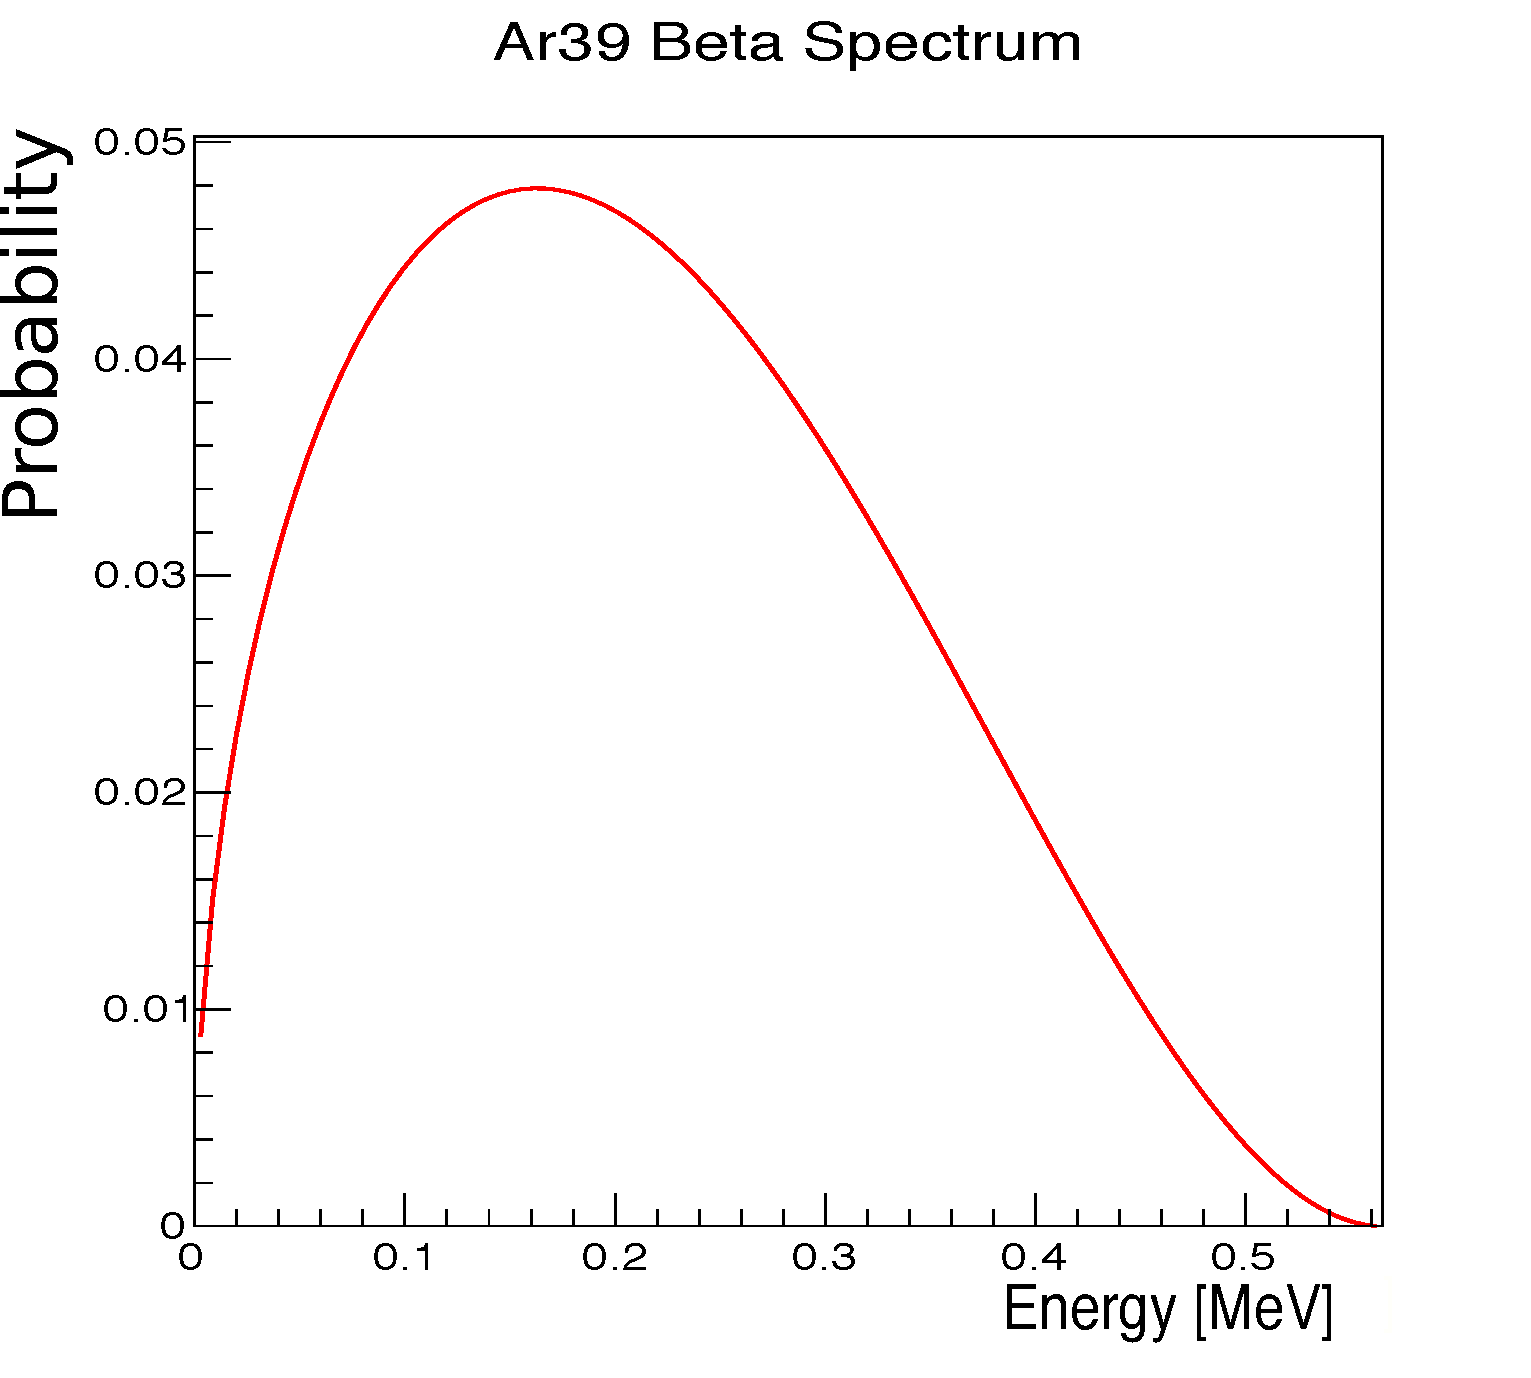
\includegraphics[width=0.45\textwidth, height=0.4\textwidth]{ar39_spectrum_larger.pdf}
\caption{$\beta$-decay spectrum of $^{39}$Ar.}\label{ar_spectrum}
\end{figure}

In general, the $^{39}$Ar events should not be a problem for beam neutrino events, as the energies of events coming from BNB or NuMI neutrino interactions will be much higher, and benefit from being in coincidence with the beam gate. Supernova neutrinos on the other hand, will be very few and have an energy of no more than 50 MeV (Figure \ref{sn_spectrum}). The spectrum assumes a supernova model with complete Boltzmann neutrino transport and spherical symmetry \cite{sn_spectrum}. For a given supernova, detectors the size of MicroBooNE and SBND can expect on the order of 10 supernova neutrinos total at 1 kpc. This is compared to $^{39}$Ar events, where in 1 second a detector of SBND's size can expect around 56,000 decays in a single TPC. Although the background rate is significantly higher, each supernova event interacts with roughly a factor 10 or more energy.

\begin{figure}[H]
\center
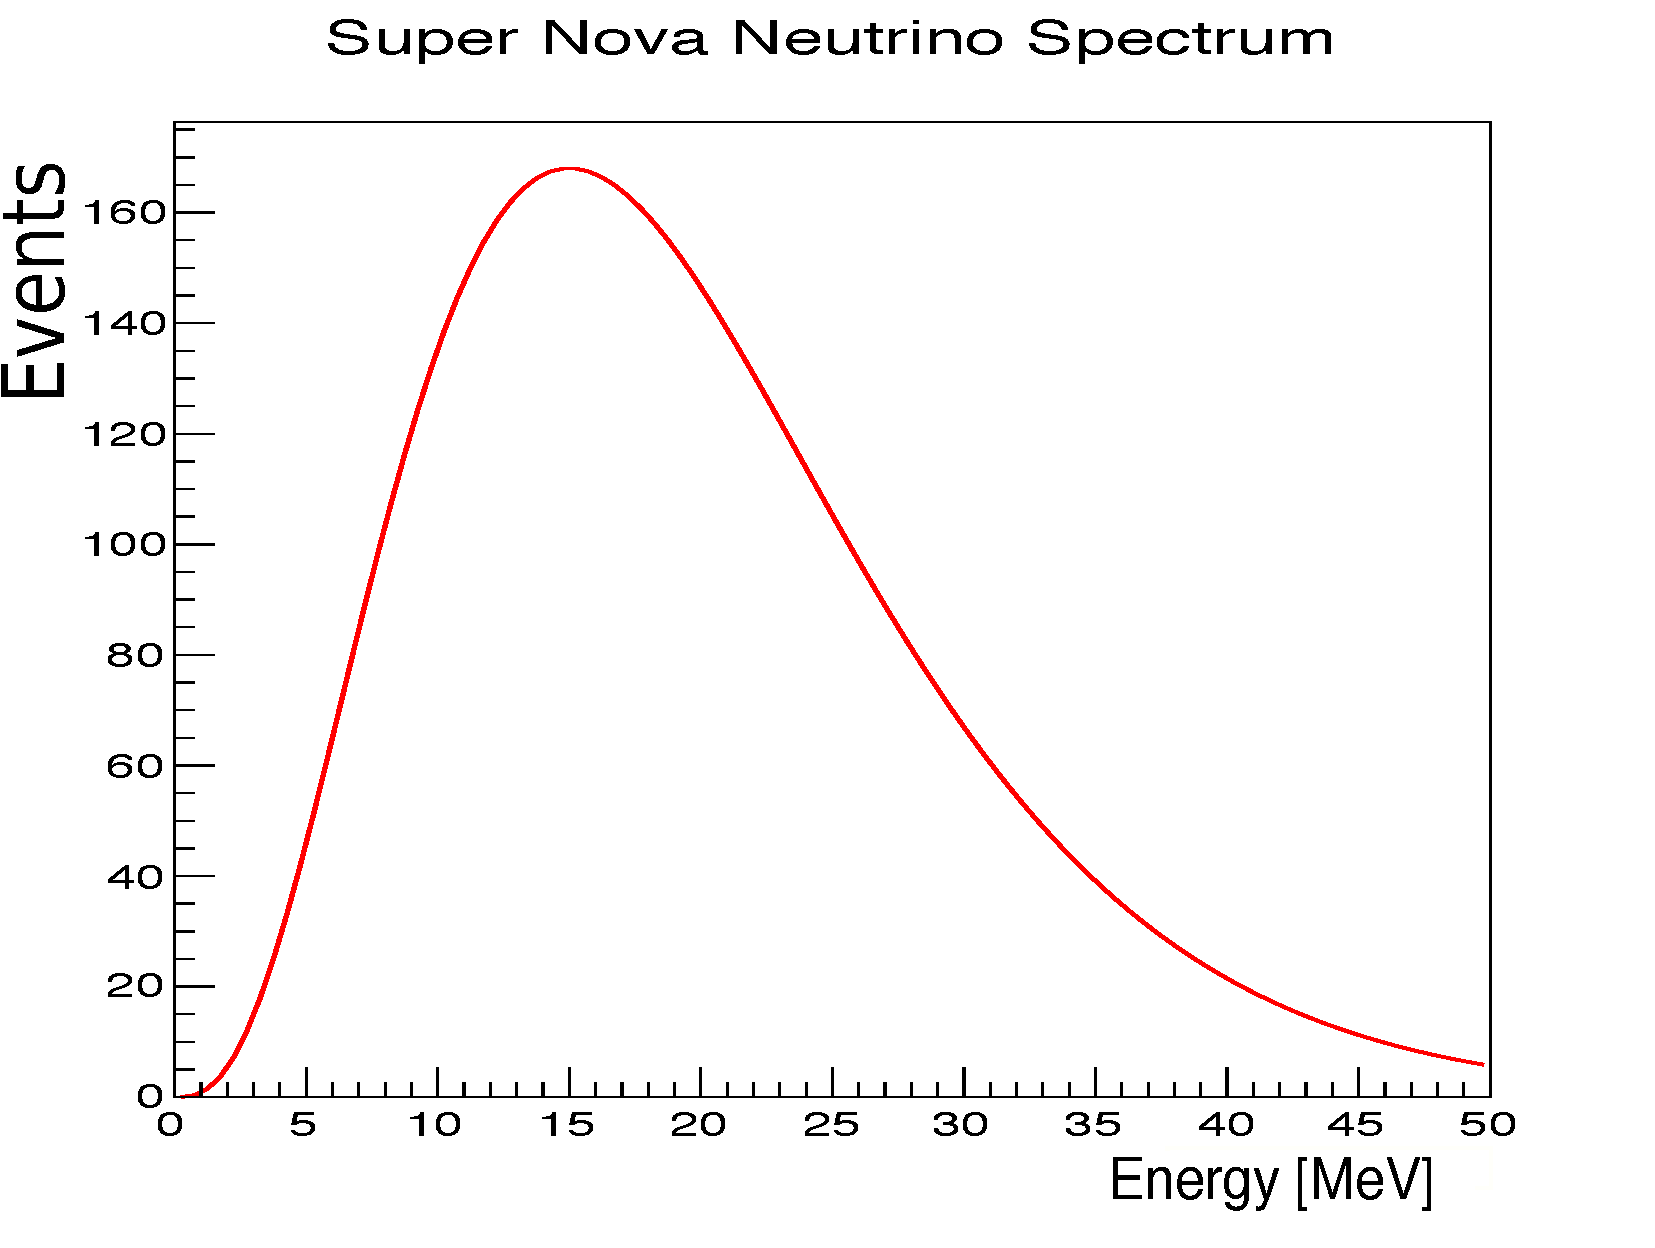
\includegraphics[width=0.45\textwidth, height=0.4\textwidth]{sn_spectrum_larger.pdf}
\caption{Expected energy spectrum of interacting neutrinos for galactic supernova neutrino flux \cite{sn_spectrum}.}\label{sn_spectrum}
\end{figure}

%The concern for detecting supernova neutrino events lies with the relative amount of background compared to the stronger, but fewer, supernova neutrino events. Sections \ref{sim_detail} and \ref{limiting_bkg} discuss the details of a simulation written to compare the $^{39}$Ar background and supernova neutrinos as well as conclusions drawn from the simulation regarding removing the background signal.

\section{Simulation Details}\label{sim_detail}

The simulation used here builds on work done in the tech note DocDB \#1155, including great detail about the fast optical simulation, validation, and characteristics of scintillation light in SBND. Work described here focuses more on the application of the simulation.

\subsection{Fast Optical Simulation}
The background scintillation light produced by $^{39}$Ar in a liquid argon TPC can be modelled by making use of fast optical simulation libraries. These libraries function as look-up tables for the ``visibility'' parameter, which is a probability that a photon originating at a specific location in the detector reaches a given PMT. This method is particularly useful, as tracking each generated photon individually through the detector is CPU and memory intensive. The visibility is tied to the light yield of the detector, where a higher light yield configuration results in a greater number of photons detected. The different configurations covered in this note are shown in Figure \ref{light_configurations}. The configurations include
\begin{itemize}
	\item ''No foils" - TPB-coated PMTs with opaque cathode
	\item  ''Cathode only" - TPB-coated PMTs with TPB-coated reflective foils on cathode
	\item ''Full coverage" - TPB-coated PMTs with TPB-coated reflective foils on cathode and field cage
\end{itemize}

\noindent where adding further TPB-coated foils increases the light yield of the system.

\begin{figure}[H]
\center
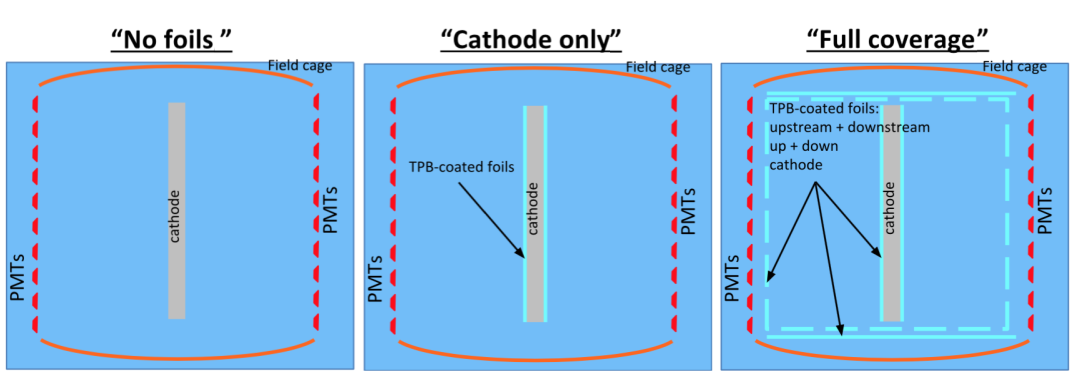
\includegraphics[width=0.8\textwidth]{configurations.png}
\caption{Light detection system configurations considered in this note. (Left) No TPB reflecting foils, only TPB on the PMTs. (Centre) Opaque cathode covered with TPB reflecting foil. (Right) Field cage and cathode covered with foils.}\label{light_configurations}
\end{figure}

The libraries make use of voxelisation to discretise the location of a photon inside the detector. In the cases where TPB reflective foils are included, the library also distinguishes between direct and reflected visibility. In addition to the geometrical considerations, second order effects like Rayleigh scattering and a 50\% efficiency for direct light incident on the PMT, due to TPB re-emission are already included. Exact details can be found in DodDB \#1155.

\subsection{Photons from Low Energy Events}

The number of photons generated by an ionising particle can be expressed simply as the particle's energy deposition multiplied by a known scintillation yield, where the scintillation yield is a function of the electric field and deposition profile. Thus by including the visibility, the number of photons reaching the PMTs is calculated. This value is defined for each voxel-PMT combination. Lastly we apply the quantum efficiency for the PMTs to end up with the total number of detected photons on a PMT given an ionising particle deposits a certain amount of energy at a given location in the detector. This idea is expressed in the formula:

\begin{equation} \label{no_gamma}
N_{\gamma} = Poisson[Visibility \times dE \times SY] \times QE
\end{equation}

\noindent where SY is the scintillation yield and QE the PMT quantum efficiency. From before, given SBND's expected electric field magnitude of 500 V/cm, the scintillation yield is taken to be 24,000 $\gamma$/MeV for low mass particles. dE is the total energy the particle deposited into the medium, and Visibility a parameter extracted from the optical libraries. A typical $^{39}$Ar decay will result in up to around 50 photoelectrons integrated over all PMTs, which is small compared to a beam neutrino event.

To model the background we calculate the expected number of decays expected in a fixed amount of time from the activity of $^{39}$Ar, the mass of the liquid argon inside the detector, and the timing window:

\begin{equation} \label{no_argon}
N_{decays} = Poisson[ Activity \times time \times mass]
\end{equation}

where in this case the activity is given in Bq/kg. For example, taking the planned amount of liquid argon in one SBND TPC (56 tonne), a readout window of 1.2 ms and the activity of $^{39}$Ar of 1 Bq/kg leads to about 67 events. The decays of each $^{39}$Ar atom are treated as independent and are fluctuated by a Poisson distribution.

The visibility depends on several factors, such as the light yield of the system and the location inside the detector. With respect to the simulation, this means we select a detector configuration and randomly assign the decay a voxel within the detector volume. Finally the energy of the decay is generated from the $^{39}$Ar decay spectrum. Together with the position, Equation \ref{no_gamma} gives the number of photons generated per PMT. 

The supernova neutrino events are simulated in a similar fashion to the $^{39}$Ar events, where their location is randomly selected inside the detector and the energy spectrum is taken from \ref{sn_spectrum}. The photons of each supernova event are tracked like the photons from the $^{39}$Ar decays.

Due to the small number of supernova events distributed over a few 10s of milliseconds, each event can be tracked separately in time. Whereas many $^{39}$Ar events occur within several microseconds and may have overlapping signals. Section \ref{sim_timing} discusses how timing is implemented into the simulation.

\subsection{Simulating Timing}\label{sim_timing}

The arrival times of photons coming from events with the same energy and position can be substantially different, because photons generated by the event do not necessarily arrive at the same, due to transport effects. It is also likely that photons from two different events can arrive very close to one another in time. The fast optical simulation libraries contain a parameterised timing which accounts for effects of the propagation. Based on the wavelength of the photon and its distance, the time needed for the photon to travel from its point of origin to the PMT is calculated. The timing parameterisation is explained in detail in DocDB 1155. For the purpose of this simulation, the time each photon takes to propagate from the point of creation to the point of detection is defined as $t_{trans}$. Each photon is assigned a transport time value, where the typical time is on the order of several 10s of nanoseconds.

A larger variation of the arrival time comes from the scintillation time of the argon in the detector. As argon scintillation is governed by two separate time constants due to its singlet and triplet decay channels, this gives the emission time a spectrum between a few nanoseconds and several microseconds, seen in Figure \ref{ar40_scint}. This is also calculated per photon and will be defined as $t_{Scint}$.

\begin{figure}[H]
\center
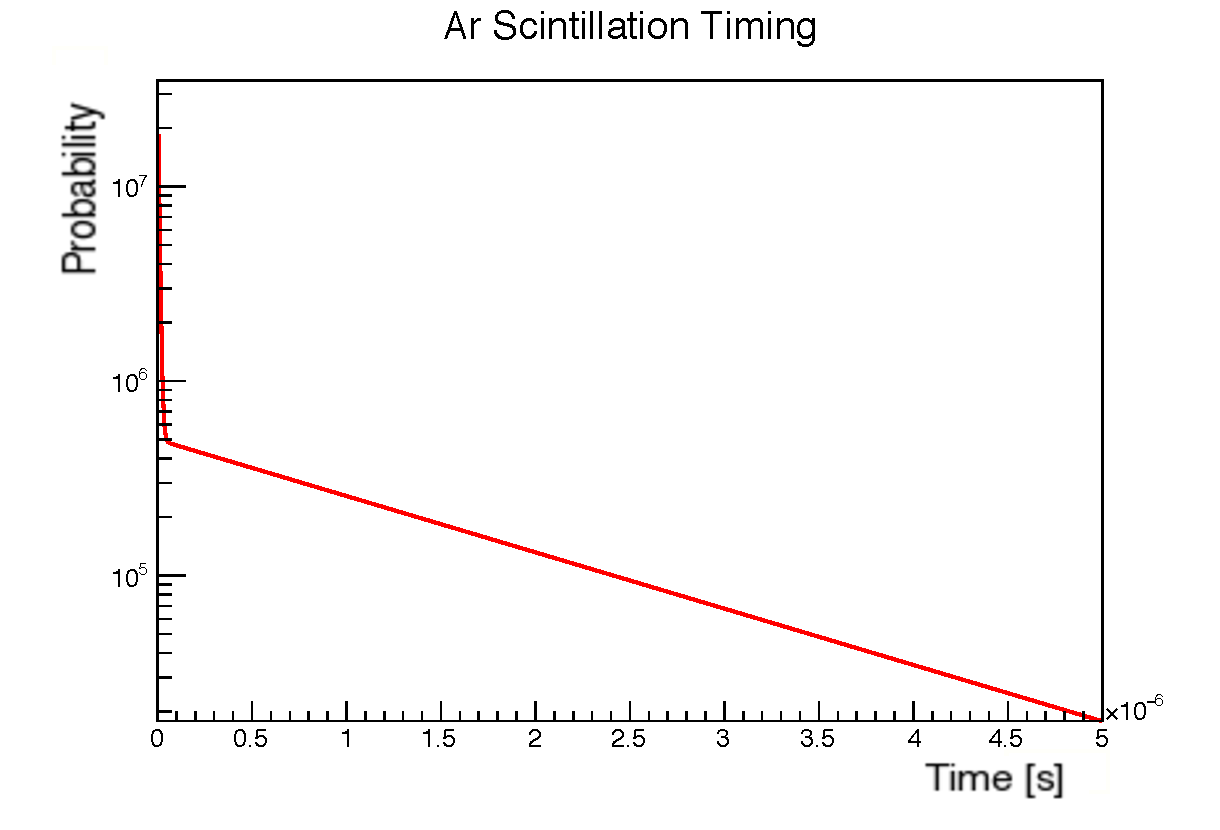
\includegraphics[width=0.5\textwidth]{ar40_scintillation_timing_larger.pdf}
\caption{Scintillation timing for argon. Note the two components, where the fast component is the singlet decay channel composing roughly 25\% of the light emitted, while the triplet decay channel composes roughly 75\%.}\label{ar40_scint}
\end{figure}

The last component for the time comes from the time of the decay. The ${39}$ Ar decays are assumed to be uniform in time, meaning $t_{Decay}$ is pulled randomly over a predetermined time window. This is calculated per event, whereas the other two components are calculated per photon. Thus the recorded time of the photoelectron is a simple sum of these three terms:

\[  t_{total} = t_{Decay} + t_{Scint} + t_{trans} \]

\noindent where $t_{total}$ is calculated per photon arriving at the PMTs. The same procedure is used for both the photons generated by $^{39}$Ar events and supernova neutrinos. By tracking the arrival times of all photons and on which PMT they arrive, we can study the effects of overlapping $^{39}$Ar events on supernova neutrino events. It should be pointed out that the simulation makes certain simplifying assumptions, such as all energy released in the $^{39}$Ar is instantly deposited inside the detector. Other simplifying assumptions include how the supernova neutrino interactions are modelled. As the intention of this simulation is not to test neutrino interaction Monte Carlo, the neutrino interactions are assumed to deposit all of their energy in a single voxel. This greatly simplifies the simulation, and should have little impact on results, as the variation in visibility between neighbouring voxels is rather small.\\ %Any others?%%

\subsection{Validating the Simulation}

In this section we use the simulation to produce ''sanity" plots to cross-check if the simulation is properly reproducing the expected response of the system. From the average energy of a supernova neutrino and the average energy of a $^{39}$Ar decay, the supernova neutrino will clearly produce a much larger signal - at least a factor 10 more photons.

\subsubsection{Independent Event Validation}

Figure \ref{pmt_maps} compares single isolated events, which provide examples of expected topologies from different events for the full foils configuration. The Figure shows the SBND PMT array for a Q-value $^{39}$Ar decay, a lower energy 5 MeV supernova neutrino, and an average value 22 MeV supernova neutrino, where each event was generated in the same voxel in the centre of the TPC. For the supernova events, PMTs much further away from the interaction point see a signal, while the overall signal for the individual $^{39}$Ar decay is small across most PMTs. The PMTs appear to be joined in the centre, which is an aspect of the presentation. Appendix \ref{alt_binning} shows an alternate binning where the PMTs in the middle are separated, although the colour becomes more difficult to distinguish.

	\begin{figure}[H]
	\center
      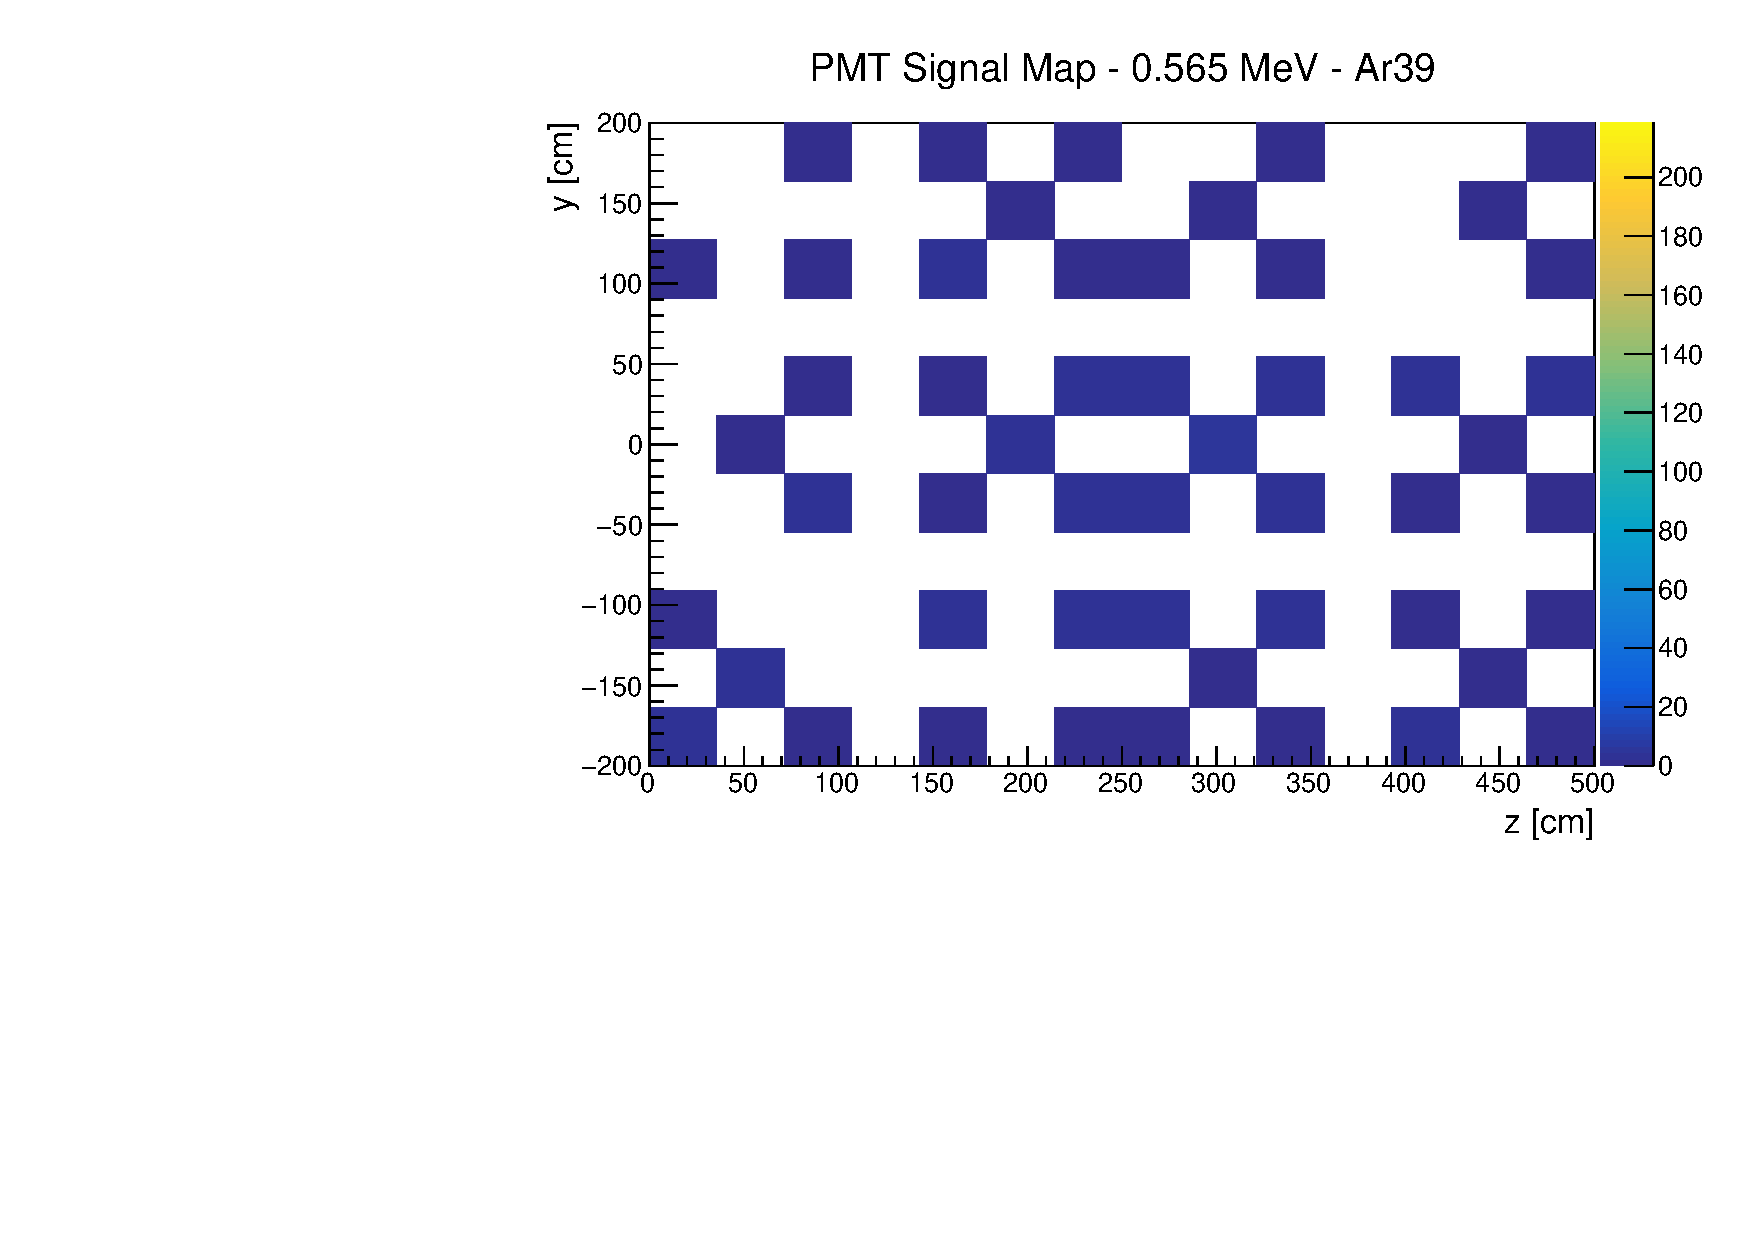
\includegraphics[width=0.43\textwidth]{pmt_maps_ar.pdf}
      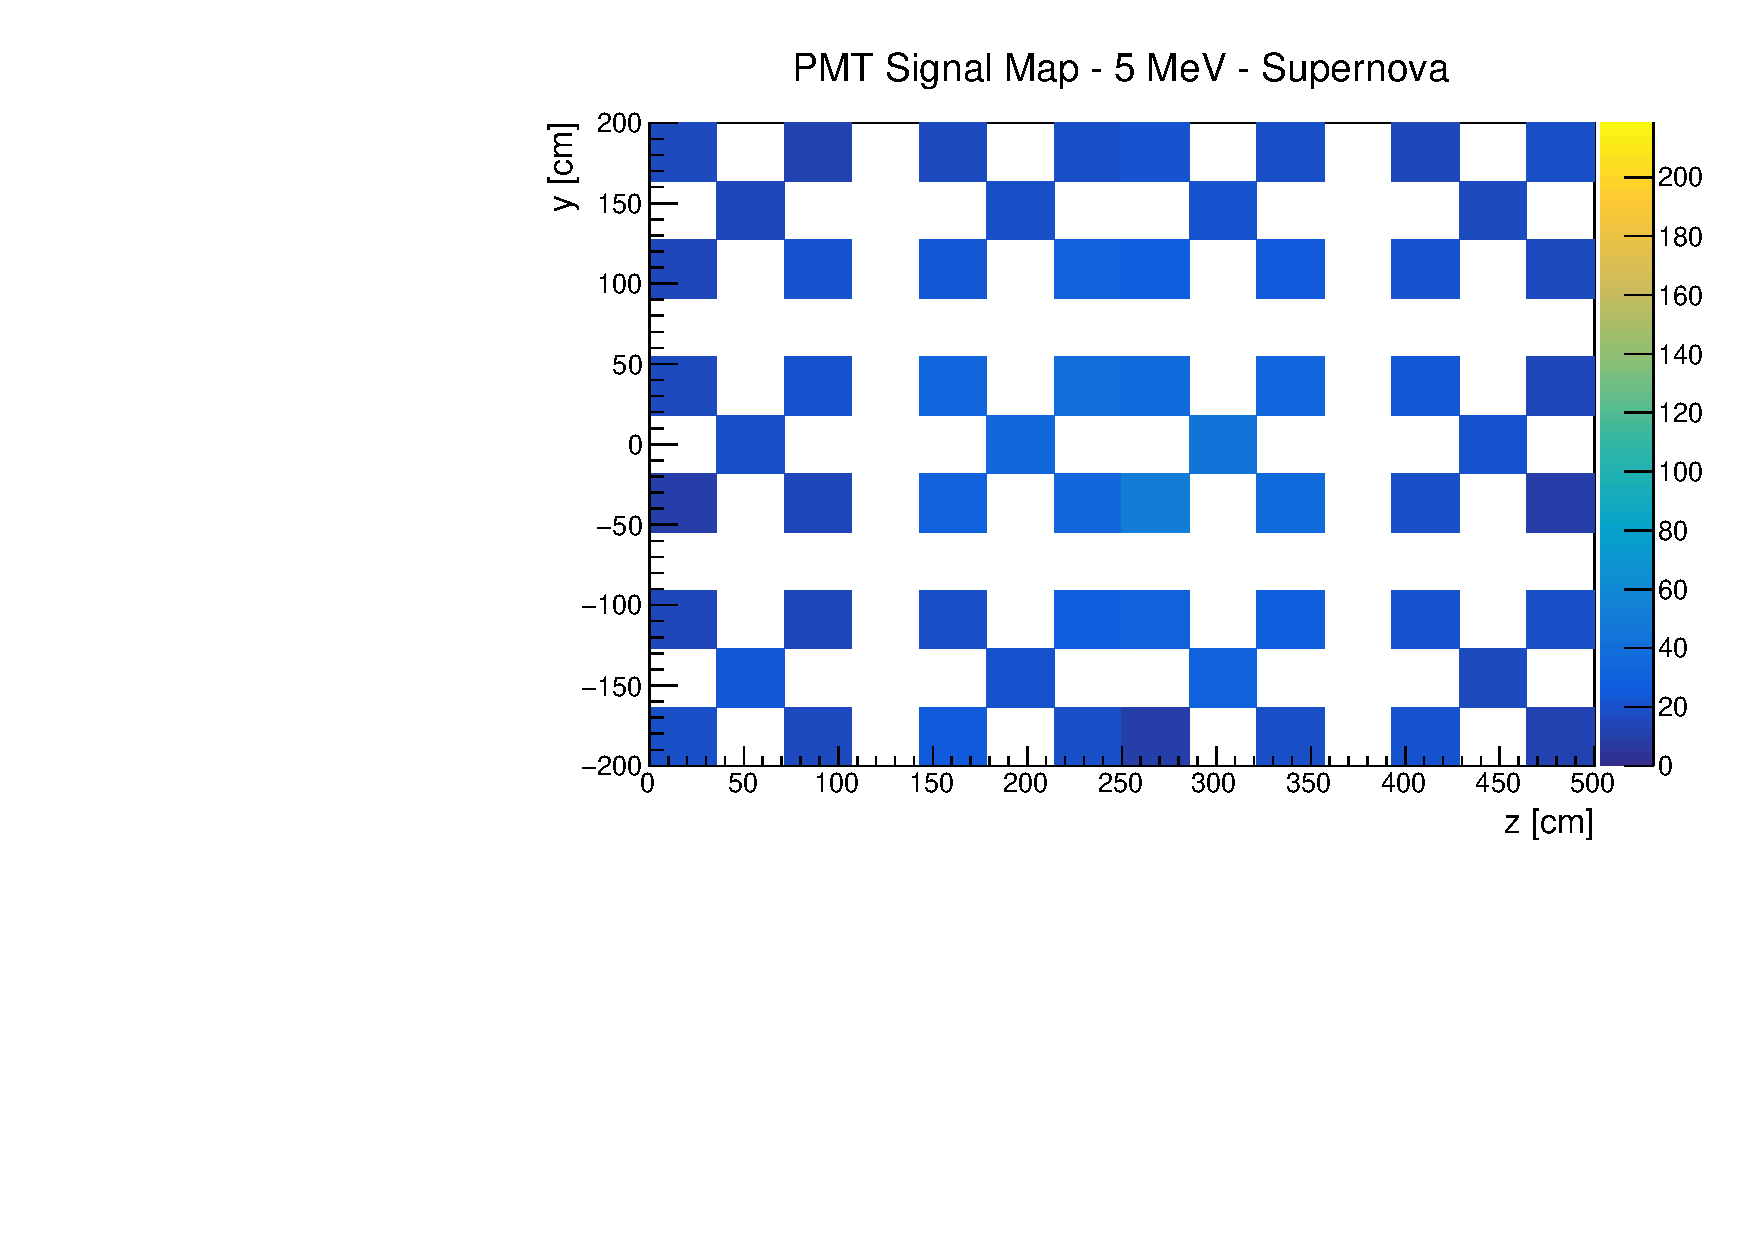
\includegraphics[width=0.43\textwidth]{pmt_maps_5_supernova.pdf}
      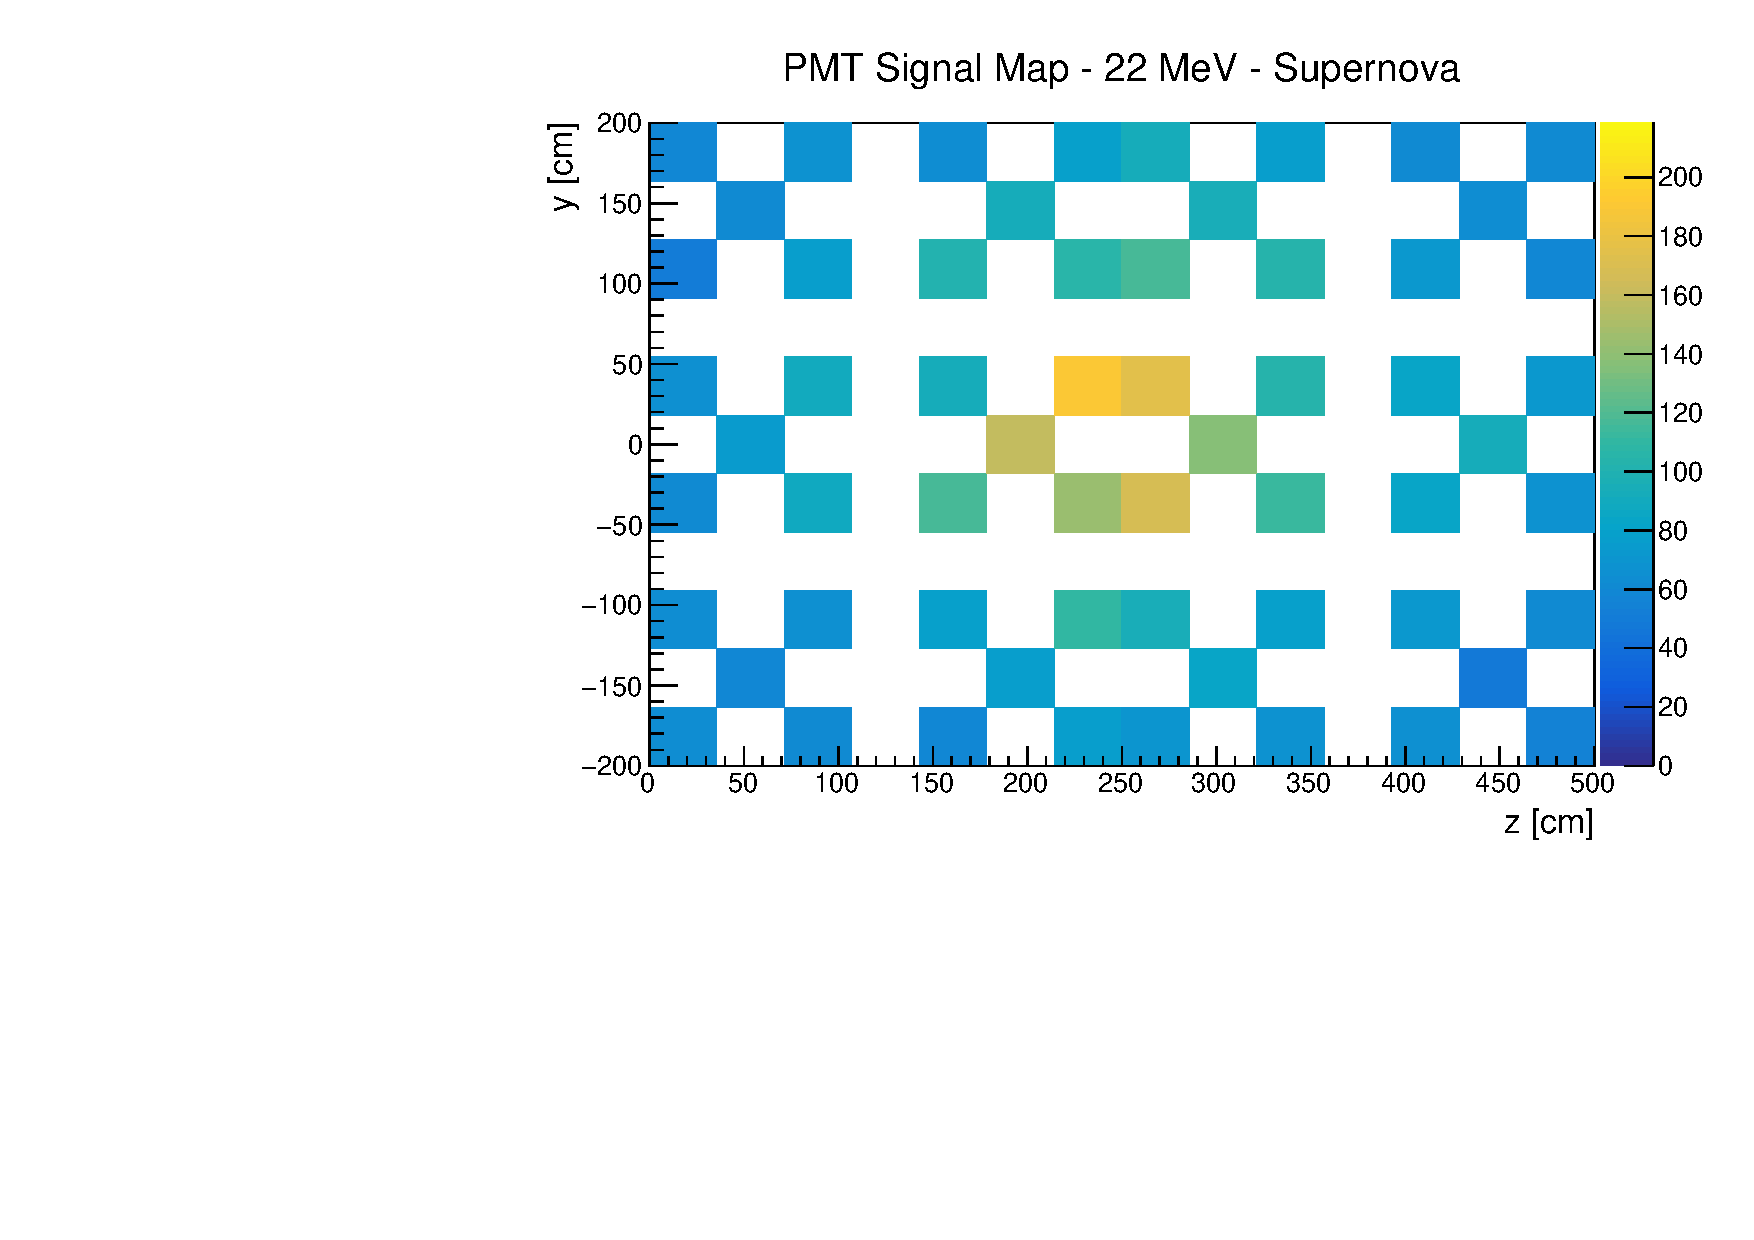
\includegraphics[width=0.43\textwidth]{pmt_maps_22_supernova.pdf}
      %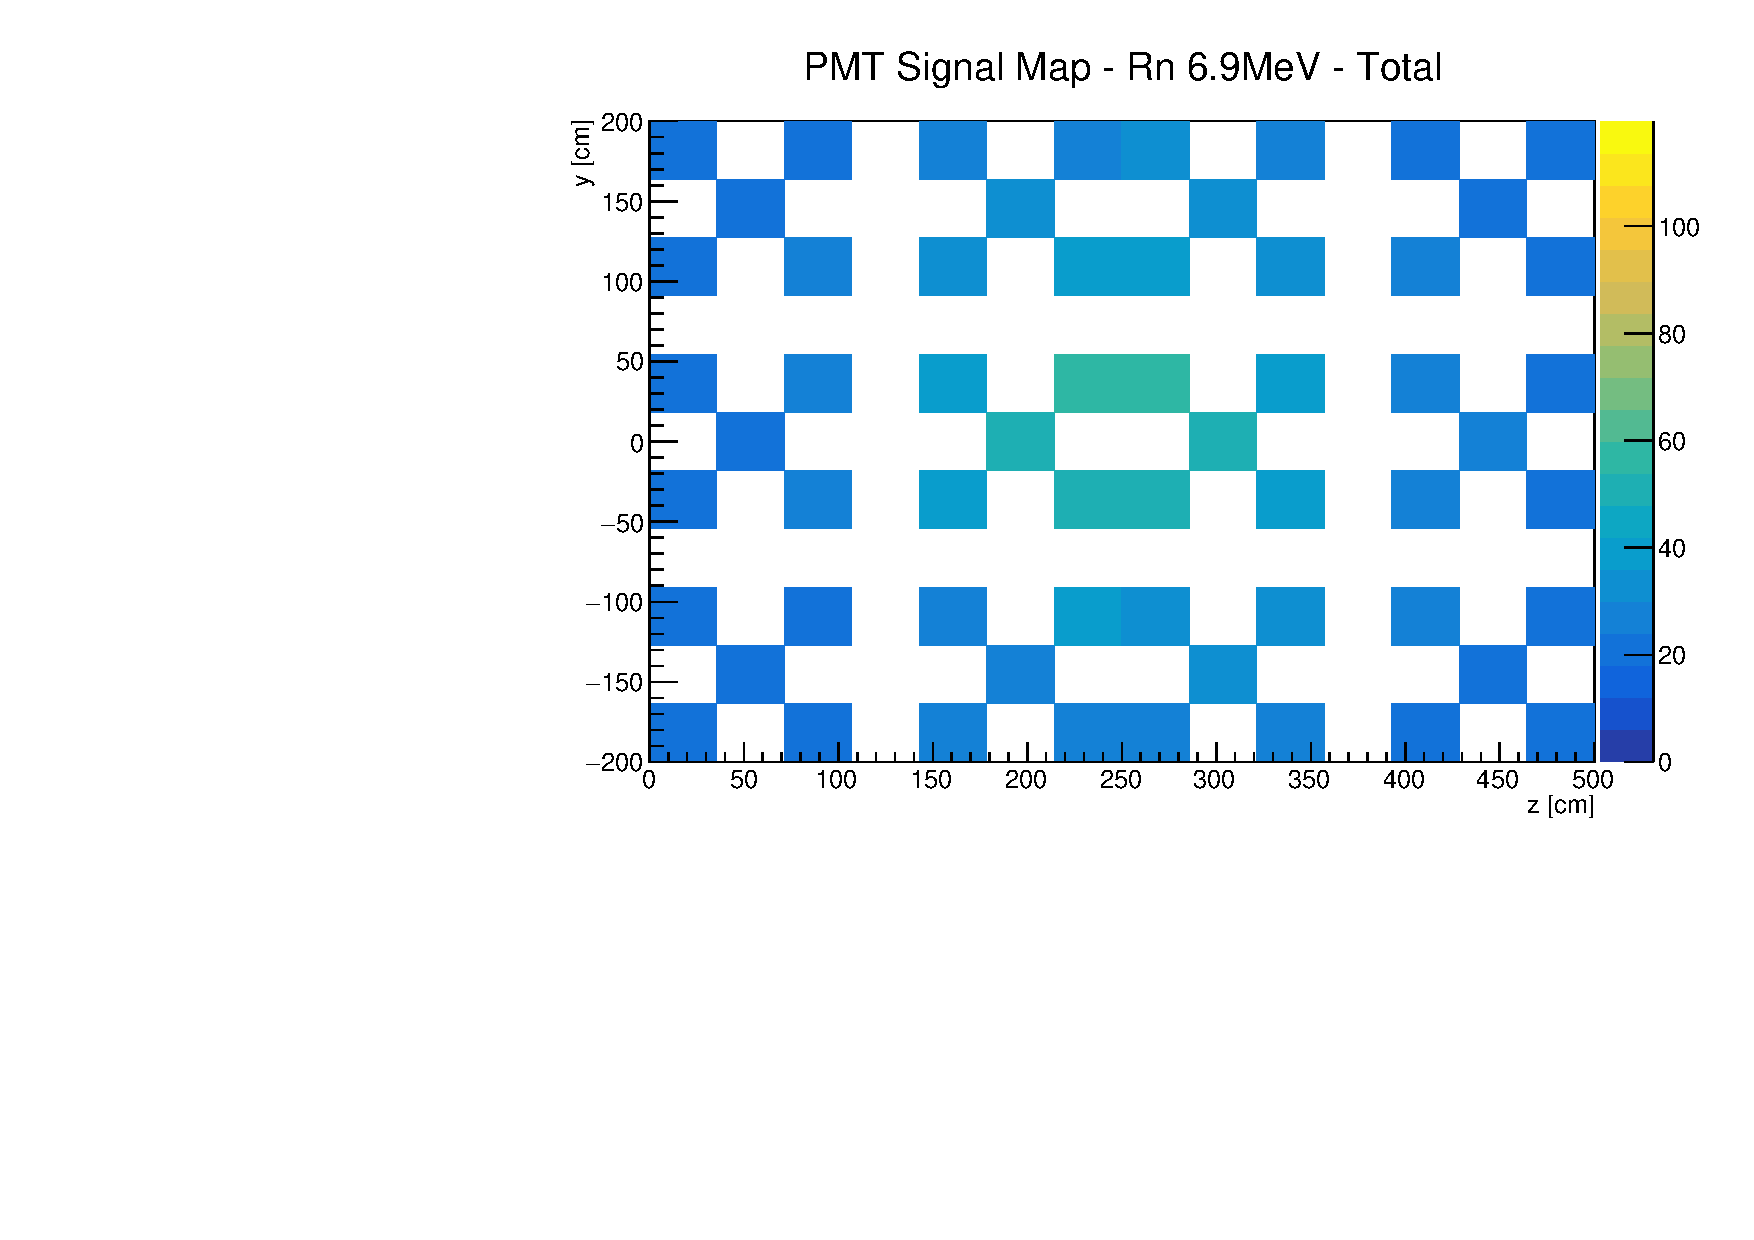
\includegraphics[width=0.43\textwidth]{rd_signal_map_foils.pdf}
	\caption{Comparison of single high-energy $^{39}$Ar, 5 MeV SN, and 22 MeV SN events in middle of detector using 60 PMTs. Single high-energy $^{39}$Ar expects about 100 hits, 5 MeV SN about 1000 hits, and 22 MeV SN about 5000 hits. Shown are the results for the total light (VUV+visible) in the case of full reflective foils. Color (z-axis) corresponds to number of photoelectons.}\label{pmt_maps}
	\end{figure}

These plots demonstrate the spatial distribution of the photoelectrons from an event as well as their intensity. When comparing even the highest energy $^{39}$Ar decays and a below average supernova neutrino, the single events can be rather clearly distinguished from one another (see Section \ref{limiting_bkg}).

\begin{figure}[H]
\center
  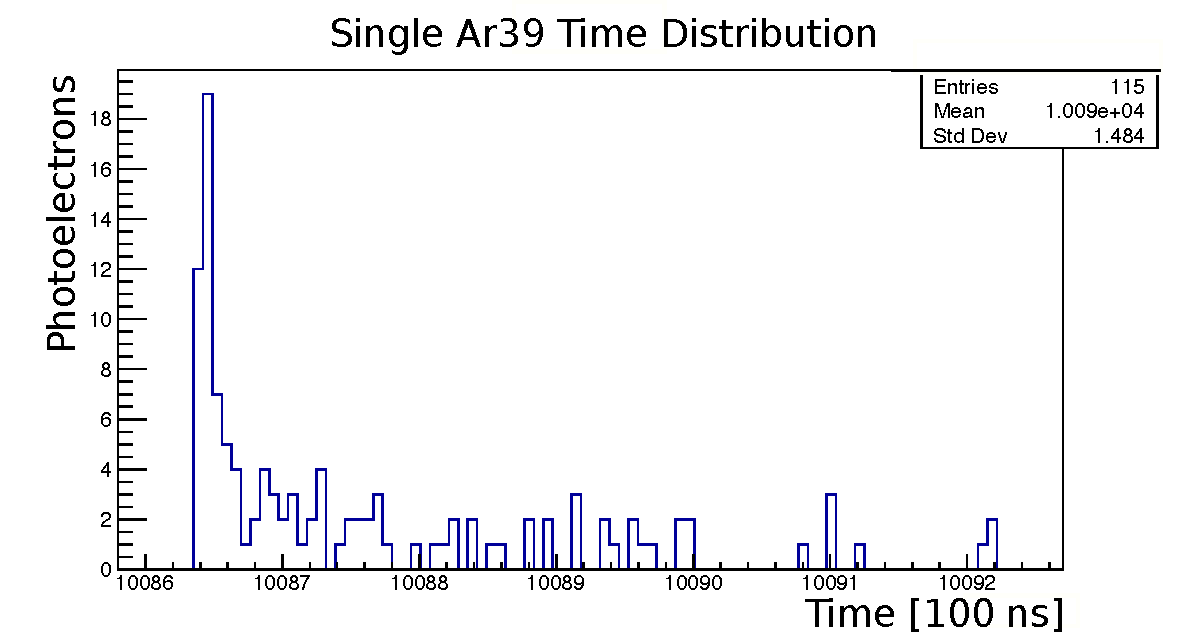
\includegraphics[width=0.43\textwidth]{single_maxE_middetector_ar_time_distribution_ff_labels.pdf}
  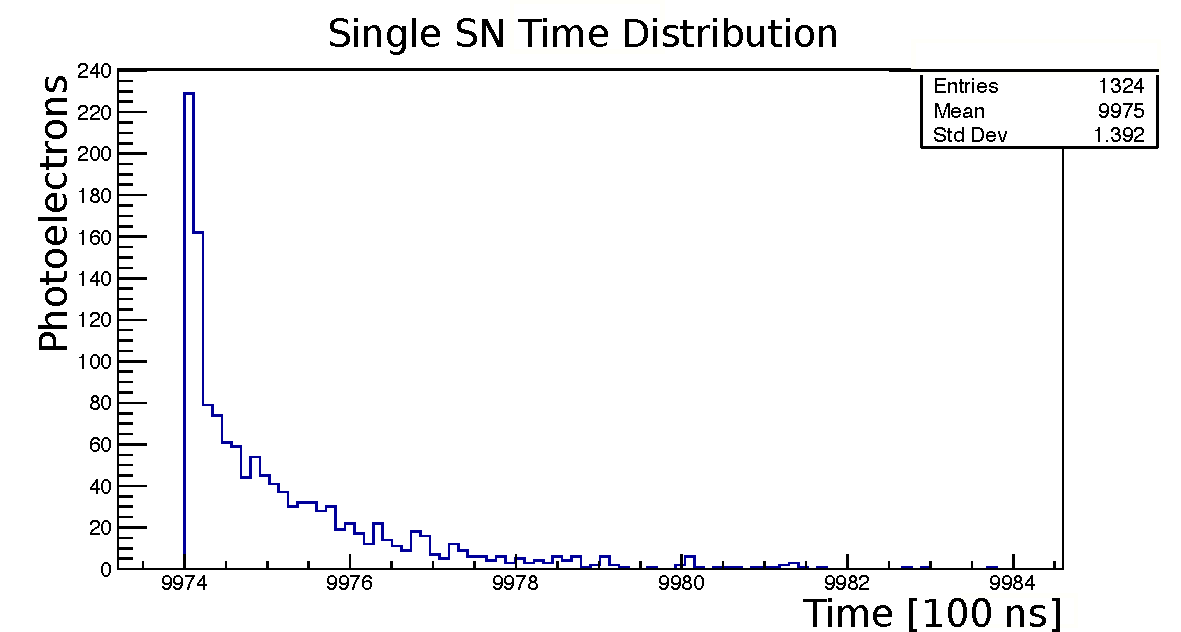
\includegraphics[width=0.43\textwidth]{single_5mev_middetector_sn_time_distribution_ff_labels.pdf}
  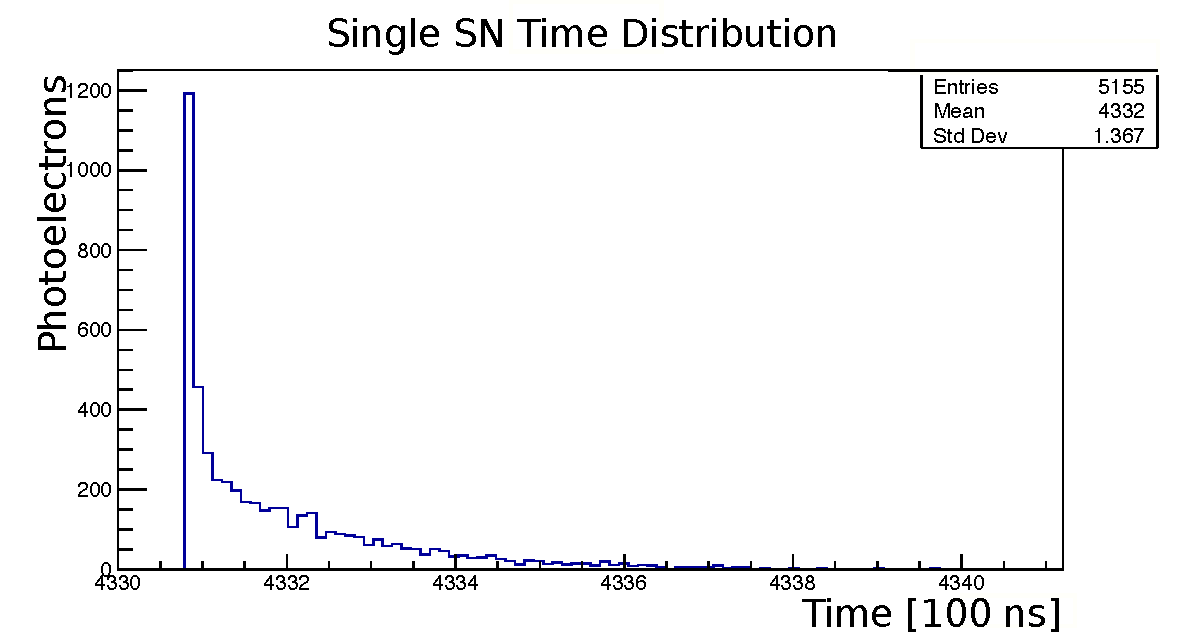
\includegraphics[width=0.43\textwidth]{single_20mev_middetector_sn_time_distribution_ff_labels.pdf}
\caption{Three different signal time ($t_{total}$) distributions all produced in the centre of the detector for the full TPB reflective foils configuration. $^{39}$Ar event with energy 0.565 MeV, supernova neutrino (up-right) with energy 5 MeV, and supernova neutrino (centre-bottom) with energy 20 MeV. Though the supernova neutrino events produce far more photons than the $^{39}$Ar decay, the timing distributions are roughly the same (start-time offset is arbitrary).}\label{single_events_timing}
\end{figure}

We can also plot the photoelectron arrival times for the full TPB reflective foils configuration are shown in Figure \ref{single_events_timing}. The factor 10 difference in energy between the single Q-value $^{39}$Ar decay and a 5 MeV supernova neutrino results in roughly factor 10 increase in overall photoelectron count. The fast and slow light components are noticeable, with a sharp peak near the first events, which tapers off. The time over which the entire signal arrives is on the order of 0.8-1.0 $\mu$s for all cases (the start-time offset is arbitrary). This time is small compared to the supernova interaction rate. However given the amount of $^{39}$Ar events and the comparatively long time constant, the background events should not be treated independently.

\subsubsection{Time Dependant Validation}

For the results shown in Section \ref{time_rejection} and beyond, each data set for $^{39}$Ar involve over $3 \times 10^{6}$ events (compared with 320,000 voxels). The individual data sets consider three different LDS configurations where TPB reflecting foils are included throughout the detector, only on the cathode, or not at all. As the location of the event in the detector changes not only the visibility, but also the transport time, it becomes increasingly important to have a large sample of events which minimise statistical fluctuations. This is most relevant for events which only produce several photoelectrons, like $^{39}$Ar. 

We apply the timing method from Section \ref{sim_timing} creating Figure \ref{pmts_time} which shows one frame of the PMT readout for the $^{39}$Ar dataset. This plot seeks to display how the structure of the decays are still visible, but that the long tails of the timing distributions will readily combine with the peaks of other decays close in time. Section \ref{time_rejection} goes on to consider rejecting the $^{39}$Ar events in-time compared to individual supernova events.

\begin{figure}[H]
\centering
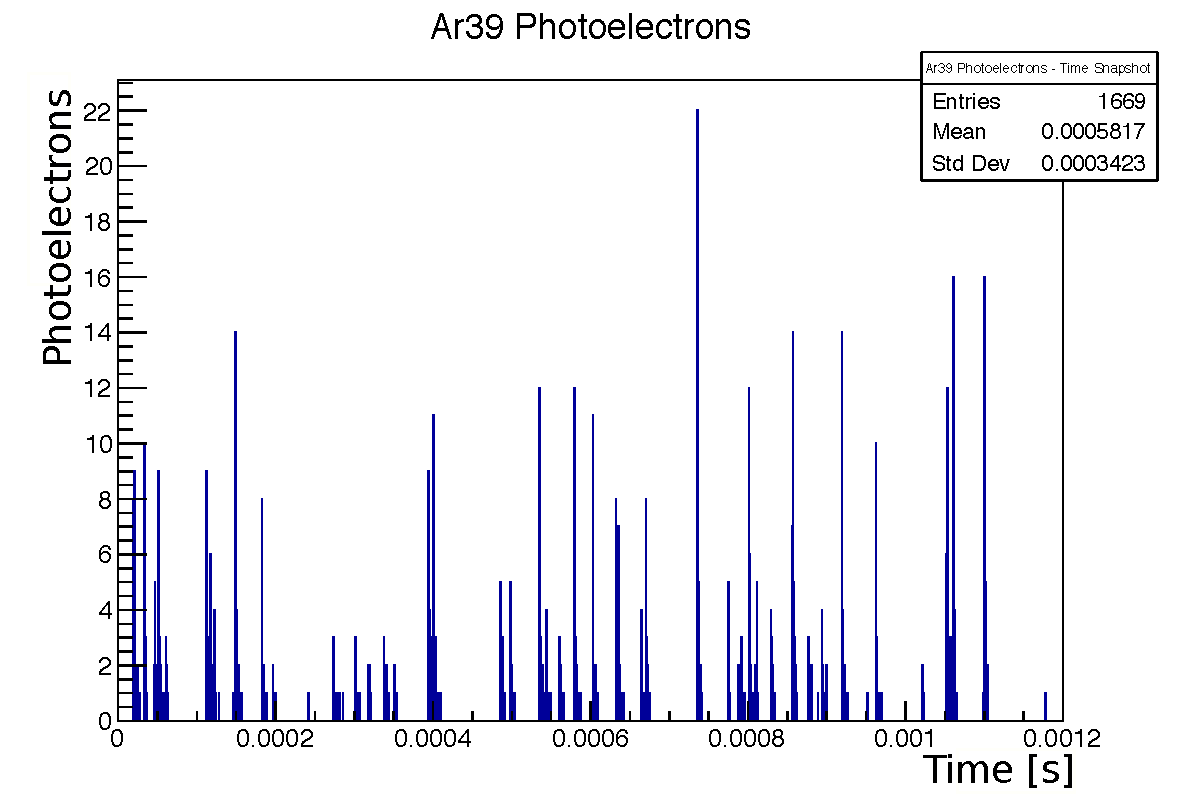
\includegraphics[width=0.45\textwidth]{pmt_times_labels.pdf}
\caption{Number of photoelectrons vs time ($t_{total}$), integrated over all 60 PMTs. The binning is in 100 ns for a time period of 1.2 ms (readout window). This is for the full TPB reflective foil configuration.}\label{pmts_time}
\end{figure}

For the large data sets, the distribution of detected photoelectrons in y (height) and z (beam-direction) was shown to be centred around the mid-way points: $y \approx 0$ and $z \approx 250$. This is because the PMTs are roughy evenly distributed in the y and z planes as well as the events being uniformly created. However when considering x (drift-direction), the light yield uniformity of the system makes a difference. Table \ref{x_table} shows the average x position. The average distance from the photocathode decreases as the light yield of the system decreases. This can also be clearly seen in Figure \ref{x_pos} for each of the three cases, where the data points correspond to detected photoelectrons.

\begin{table}[H]
	\begin{center}
	\begin{tabular}{| c || c |}
	\hline
	Configuration & Ave. X Position [cm]\\
	\hline
	 &\\
	 Full Foils & 95.14\\
	 &\\
	 Cathode & 97.31\\
	 &\\
	 No Foils & 146.4\\
	\hline
	\end{tabular}
	\end{center}
	\caption{Average drift-direction position and RMS for detected photons given different configurations.}\label{x_table}
	\end{table}

As Figures \ref{x_pos}, \ref{y_pos} and \ref{z_pos} show the number of detected photoelectrons, these plots display how the location inside the detector plays a key role for photons detection. In Figure \ref{x_pos} we observe the behaviour for the no foils setup - the visibility decreases further away from the PMT plane, resulting in few events being detected far away from the PMTs. The addition of the cathode reflector foil causes an obvious enhancement at distances greater than 140 cm, (foil located at $x = 0$) as the light coming from that region has now been wavelength-shifted by the foils and propagates as visible light inside the detector. The addition of further reflective foils for the full foils configuration results in a more uniform distribution of light, where the trough disappears. In fact, as there are no foils behind the PMT plane, the number of photoelectrons detected is largest further away from the PMTs.

  \begin{figure}[H]
    \center
    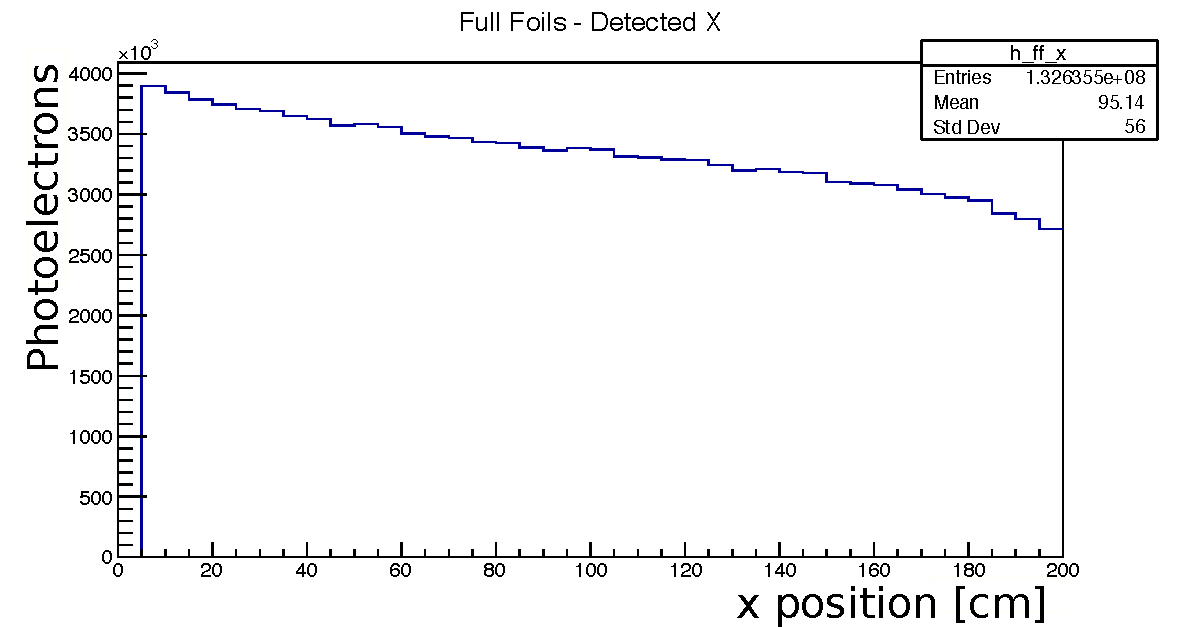
\includegraphics[width=0.48\textwidth]{detected_fullfoils_x_labels.pdf}
    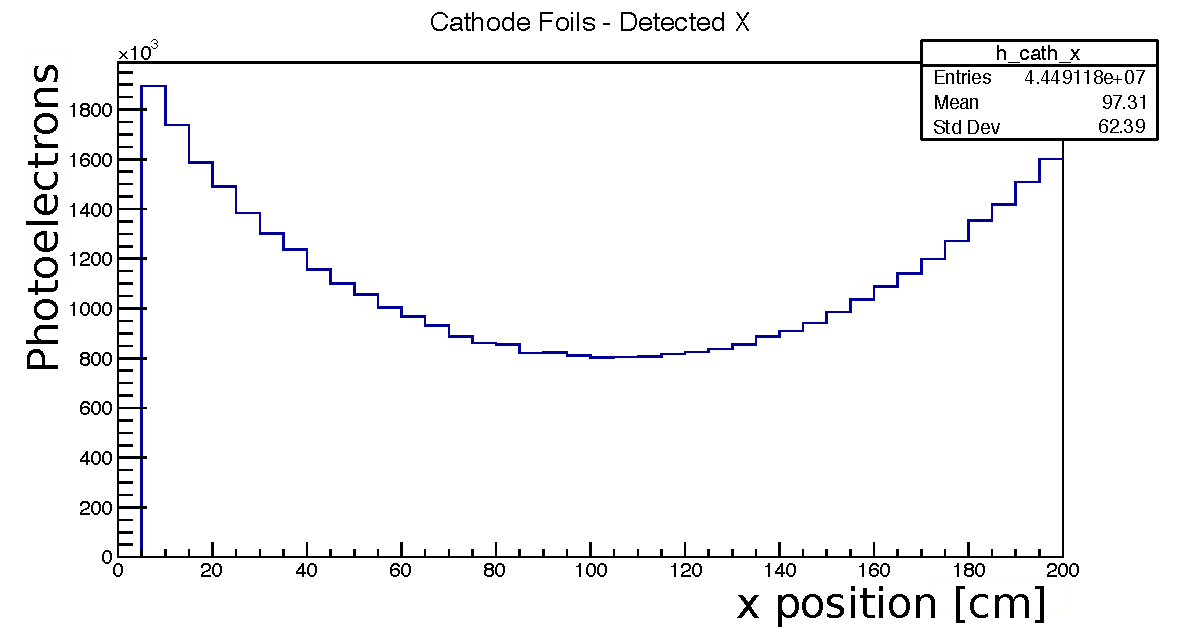
\includegraphics[width=0.48\textwidth]{detected_cathode_x_labels.pdf}
    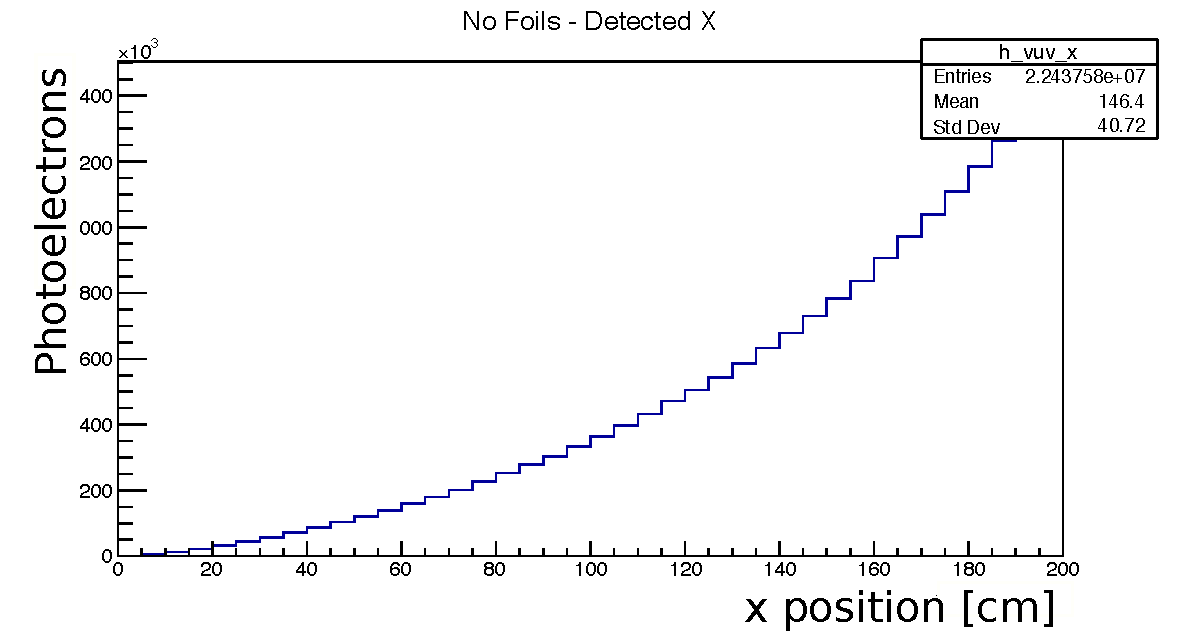
\includegraphics[width=0.48\textwidth]{detected_nofoils_x_labels.pdf}
    \caption{Detected photoelectrons versus x position in the detector.}\label{x_pos}
  \end{figure}
  
  In the y and z distributions, all three configurations have the values maximised around the centre of the detector, as would be expected. For the full foils case, we find that the events occurring near the edges of the detector have the highest number of detected photoelectrons. This is due to reflective foils close to the event origin, meaning events near the edges of the detector have a large visible light component. This is contrasted with the cathode and no foils case, where the centre of the detector sees a higher contribution. The shapes of these two cases are rather similar, where the photoelectrons produced at the edges contribute very little, and the two troughs match roughly the gap between the sets of PMTs in both the y and z directions. (See the first plot in Figure \ref{pmt_maps}) This shows that the detection of low energy $^{39}$Ar decays, in the cathode or no foils case are very sensitive to the configuration of the PMT array, and therefore the location inside the detector.
  
  \begin{figure}[H]
    \center
    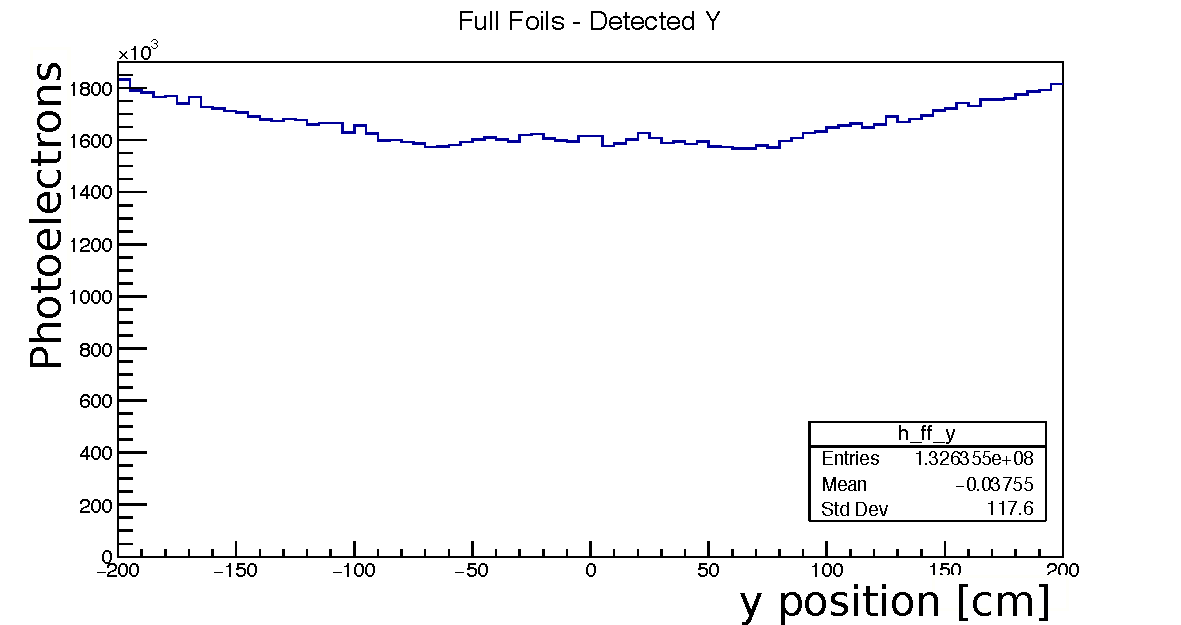
\includegraphics[width=0.48\textwidth]{detected_fullfoils_y_labels.pdf}
    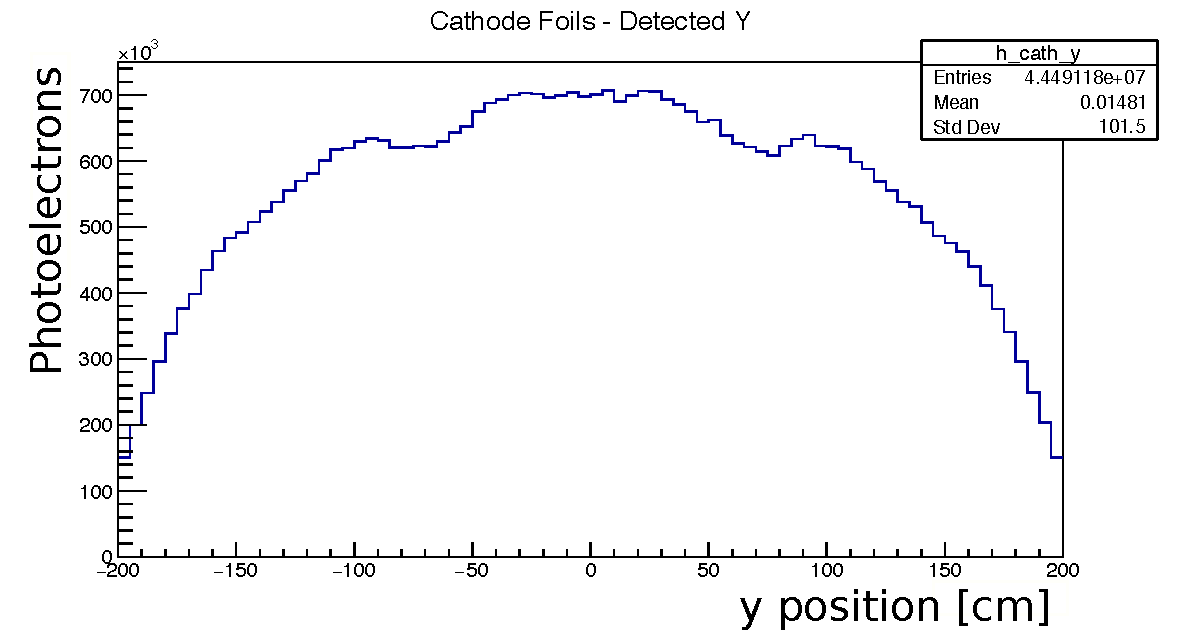
\includegraphics[width=0.48\textwidth]{detected_cathode_y_labels.pdf}
    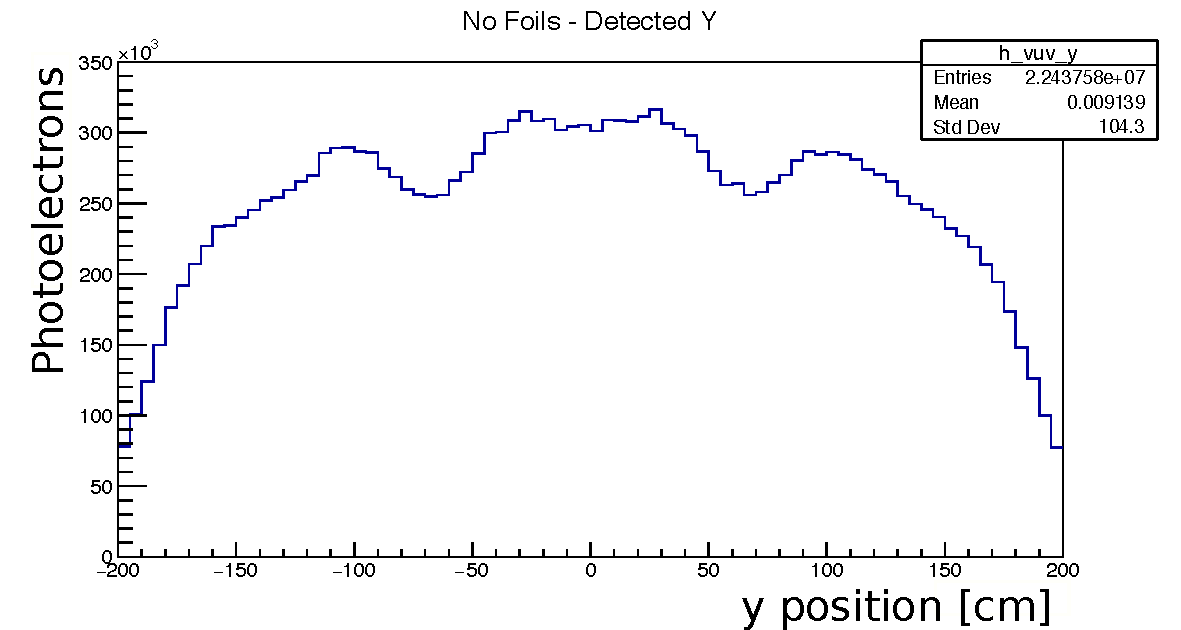
\includegraphics[width=0.48\textwidth]{detected_nofoils_y_labels.pdf}
    \caption{Detected photoelectrons versus y position in the detector.}\label{y_pos}
  \end{figure}
  
    \begin{figure}[H]
    \center
    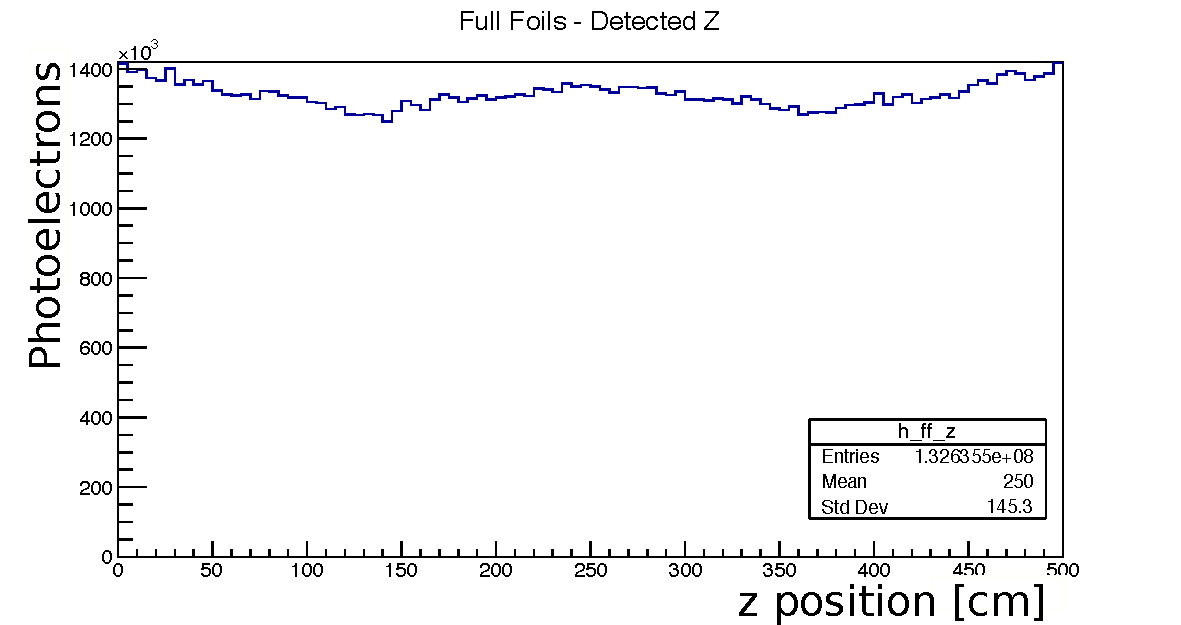
\includegraphics[width=0.48\textwidth]{detected_fullfoils_z_labels.pdf}
    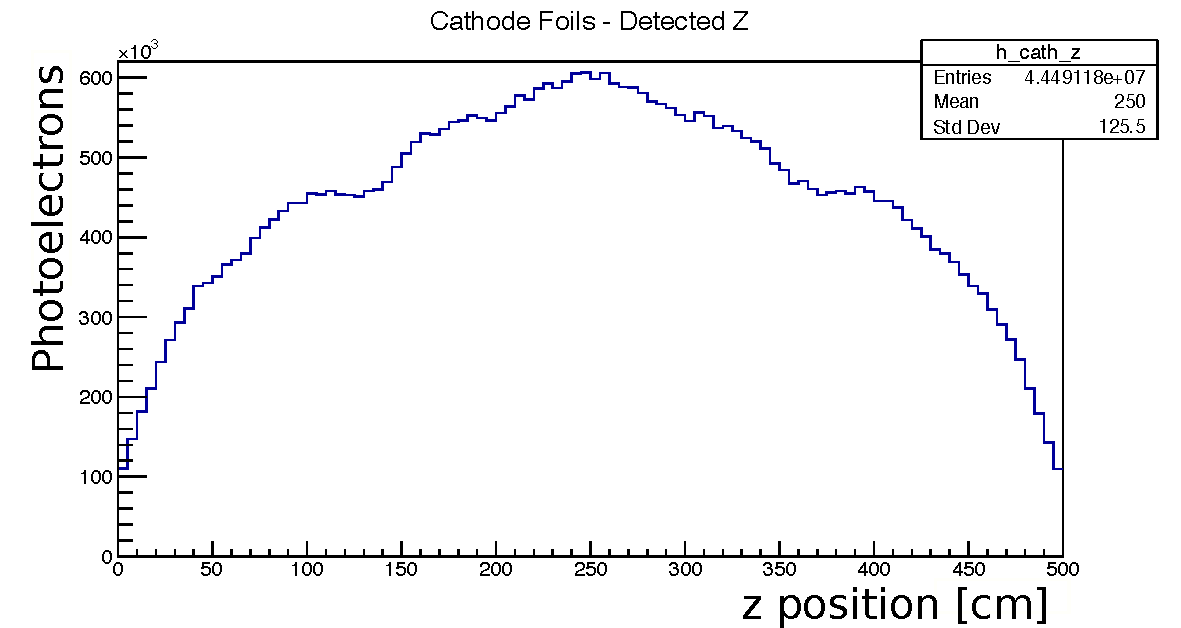
\includegraphics[width=0.48\textwidth]{detected_cathode_z_labels.pdf}
    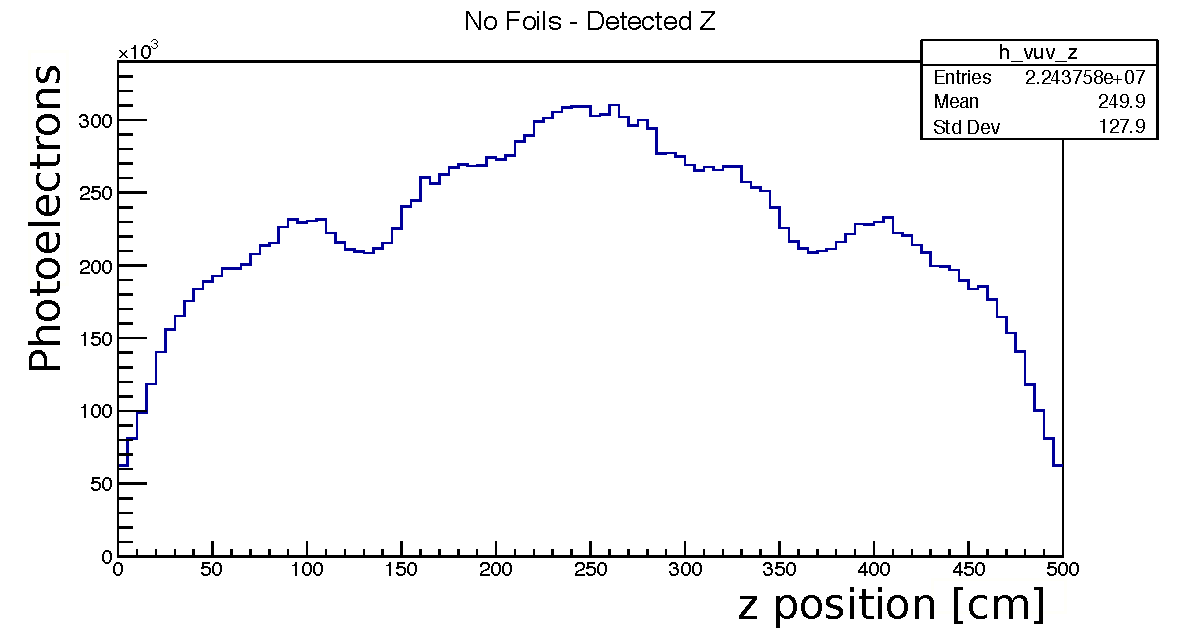
\includegraphics[width=0.48\textwidth]{detected_nofoils_z_labels.pdf}
    \caption{Detected photoelectrons versus z position in the detector}\label{z_pos}
  \end{figure}
%%%%%%%%%%%%%%%%%%%%%%%%%%%%%%%%%%%%%%%%%%%%%%%%%%%%%%%

%Separate from $^{39}$Ar, but potentially another background, are two of Radon's $\alpha$-decays. Rn decays to $^{216}$ Po emitting 6.906 MeV and $^{212}$Po emitting 8.955 MeV, energies at which the lower energy supernova neutrinos would be faked or obscured. The contamination of Rn inside the MicroBooNE detector is currently under investigation, however $\alpha$ and $\beta$ events could be be discernible from one another by examining the dE/dx information, as well as the ratio of fast-to-slow light for the signal decay time \cite{borexino}.

\section{Limiting Background Signals} 

The number of expected supernova neutrino events for a liquid argon detector the size of SBND is small, in order to unambiguously observe them, a high trigger efficiency is necissary. This section outlines some $^{39}$Ar background and simulated supernova neutrino events as outlined in Section \ref{sim_detail}. First we consider $^{39}$Ar decays as independent in time, and we assume all of its photons arrive simultaneously. Despite being unphysical in that the $^{39}$Ar decays will actually overlap, this test is demonstrative of the different features of single $^{39}$Ar and supernova events and how a basic minimum threshold trigger cuts the background spectrum. We then constrain single events to the first 100 nanoseconds of their signal, rather than the total light for each event. This is meant to correspond to the ``fast light" arriving from an event in the usual trigger window. Finally we examine what happens when photons from different $^{39}$Ar decays are allowed to overlap in time, and how a similar cut to the single events case can prevent triggering falsely on background.

\subsection{Time Independent Cut Efficiencies}\label{limiting_bkg}

We first look at single events counting their total energies. This is the simplest case and further elements are added in the next sections. The format of the cut for this simple case is outlined in two parts:

\begin{itemize}
	\item Variable individual PMT threshold
	\item Variable number of individual PMTs
\end{itemize}

\noindent where the individual PMT thresholds are uniform across all PMTs. An example cut could involve at least 3 PMTs each measuring 2+ photoelectrons apiece (giving a minimum of 6 photoelectrons). The supernova events are of higher energy than the $^{39}$Ar, meaning the supernova events will typically produce more signal. Thus by increasing either the number of PMTs or the individual PMT thresholds, we expect to see only higher energy events.

Table \ref{cuts_table} outlines the basic cuts and amount of the signal/background removed by the cut for both the full reflective foil and no reflective foil configurations. Taken from a sample size with statistical uncertainty of about $1.7\%$, the cuts for this initial study erred on the side of being overly conservative. While these cuts serve as preliminary guidelines, further studies outlined in Section \ref{time_rejection} deal with considerably larger statistics. Several of these cuts are implemented in plots below. As a note, the final cut is modified for the VUV only case. Without the wavelength-shifting foils, the total amount of signal both from $^{39}$Ar and from potential supernova neutrinos is reduced. 
 
\begin{table}[H]
	\begin{center}
	\begin{tabular}{| c | c || c | c || c | c |}
	\hline
	No. PE & No. PMT & $\%$ $^{39}$Ar & $\%$ $^{39}$Ar VUV & $\%$ SN & $\%$ SN VUV \\
	\hline
	 & & & & &\\
	 1 & 1 & 40.2  & 84.5 & 0.01 & 0.01\\
	 & & & & &\\
	 2 & 1 & 60.3 & 88.8 & 0.01 & 0.2\\
	 & & & & &\\
	 2 & 2 & 70.7 & 90.2 & 0.01 & 0.2\\
	  & & & & &\\
	 3 & 2 & 87.4 & 92.9 & 0.01 & 0.4\\
	 & & & & &\\
	 3 & 3 &  92.0 & 97.9 & 0.01 & 0.6\\
	 & & & & &\\
	 3 & 4 & 95.2 & X & 0.01 & X\\
	 & & & & &\\
	 4 & 2 & 96.8 & X & 0.01 & X\\
	 & & & & &\\
	 4 & 3 & 96.8 & X & 0.01 & X\\
	 & & & & &\\
	 5 & 3 & 97.4 & X & 0.01 & X\\
	\hline
	\end{tabular}
	\end{center}
	\caption{\% Reduction in signal and background compared for the full reflective foil and no reflective foils configurations. ``VUV'' indicates the no reflective foil case and ``X'' indicates that the cut is not relevant for this case.}\label{cuts_table}
	\end{table}

By performing a simple cut of several photoelectrons incident over a few PMTs there is only a small reduction in supernova neutrino signal, but a significant reduction in the $^{39}$Ar background. Figure \ref{scint_energy_cuts} and \ref{scint_energy_cuts_vuv} visualise how these cuts affect the $^{39}$Ar and supernova neutrino energy spectra for the full foil and no foil cases.

\begin{figure}[H]
\center
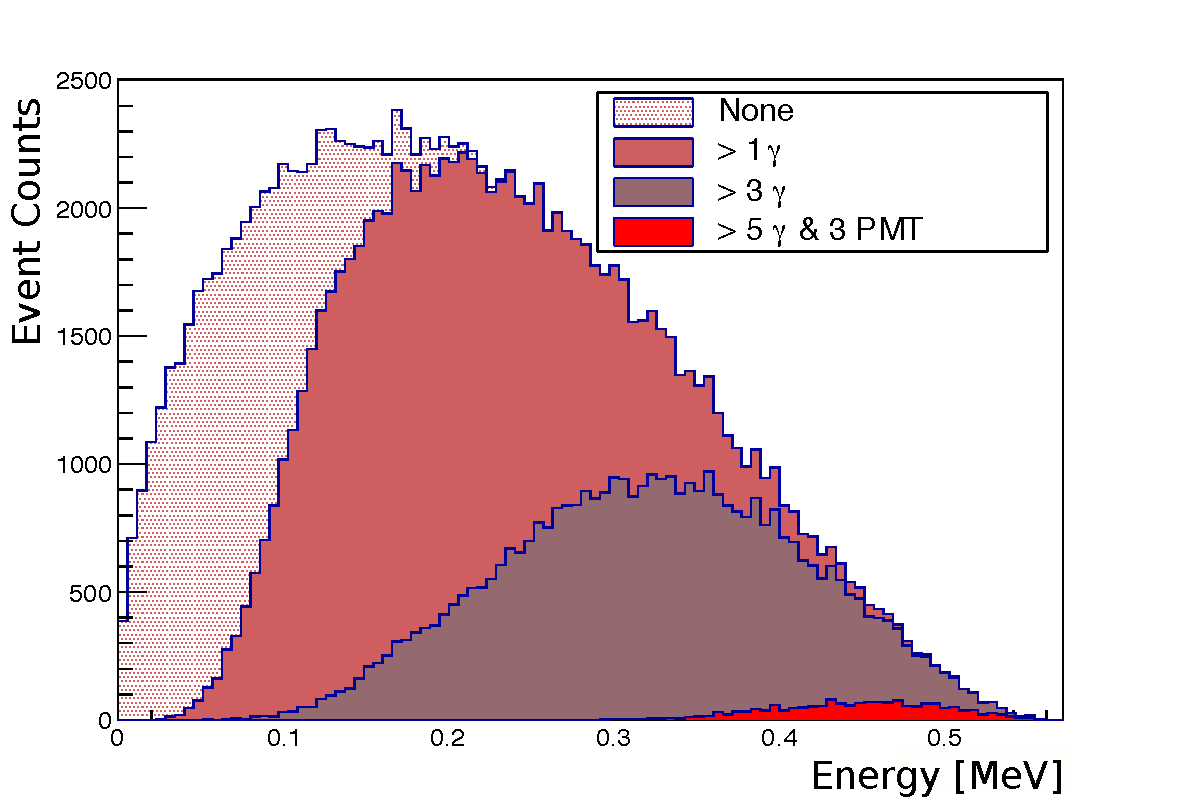
\includegraphics[width=0.45\textwidth]{ar39_energy_spectrum_60pmts_alllight_labels.pdf}
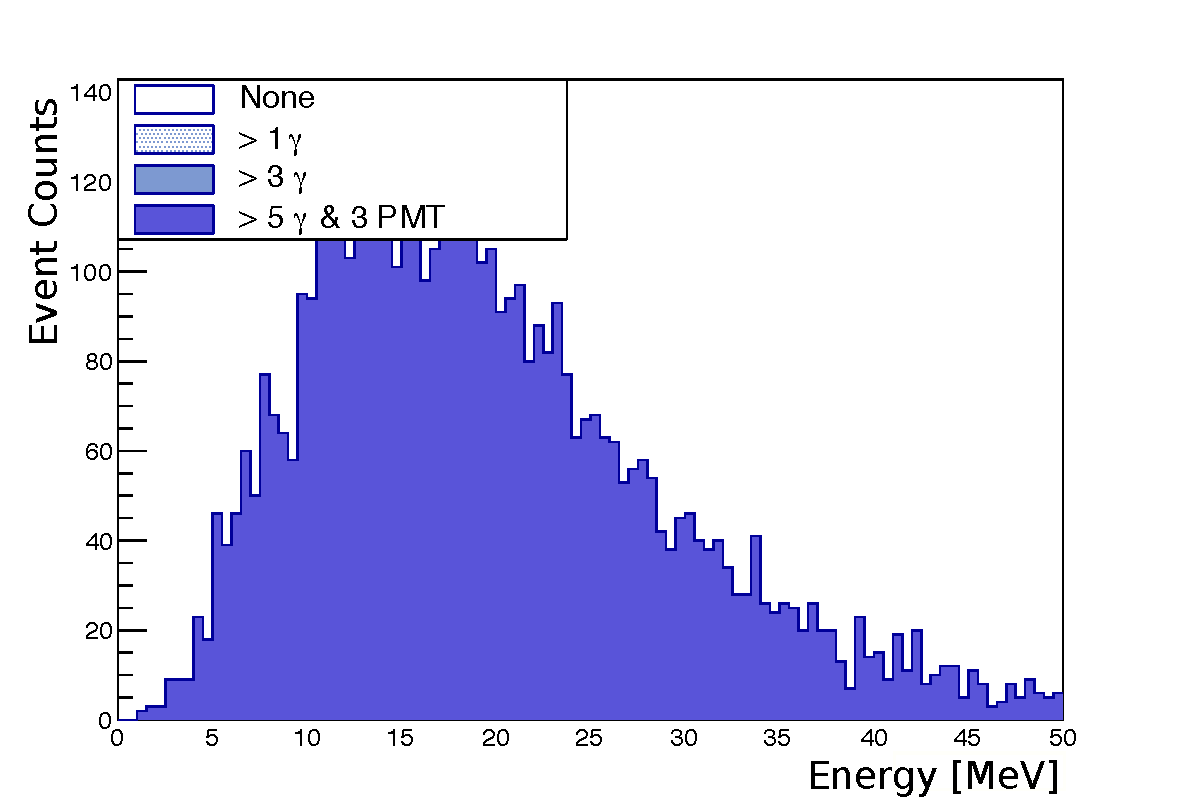
\includegraphics[width=0.45\textwidth]{sn_energy_spectrum_60pmts_alllight_labels.pdf}
\caption{Energy spectra for $^{39}$Ar and supernova neutrinos, assuming a large statistics sample for both, to observe how cuts on the number of photoelectrons per a number of PMTs modify the spectra. This case assumes a full coverage of reflective foils, and considers the contribution from both direct VUV and reflected visible light. The goal for the $^{39}$Ar spectrum is to remove it completely through these cuts, and therefore almost disappears from the plot in the case of the most aggressive cuts. Legend shows cuts where ''1 $\gamma$" corresponds to the cut 1 photoelectron on 1 PMT.}\label{scint_energy_cuts}
\end{figure}

\begin{figure}[H]
\center
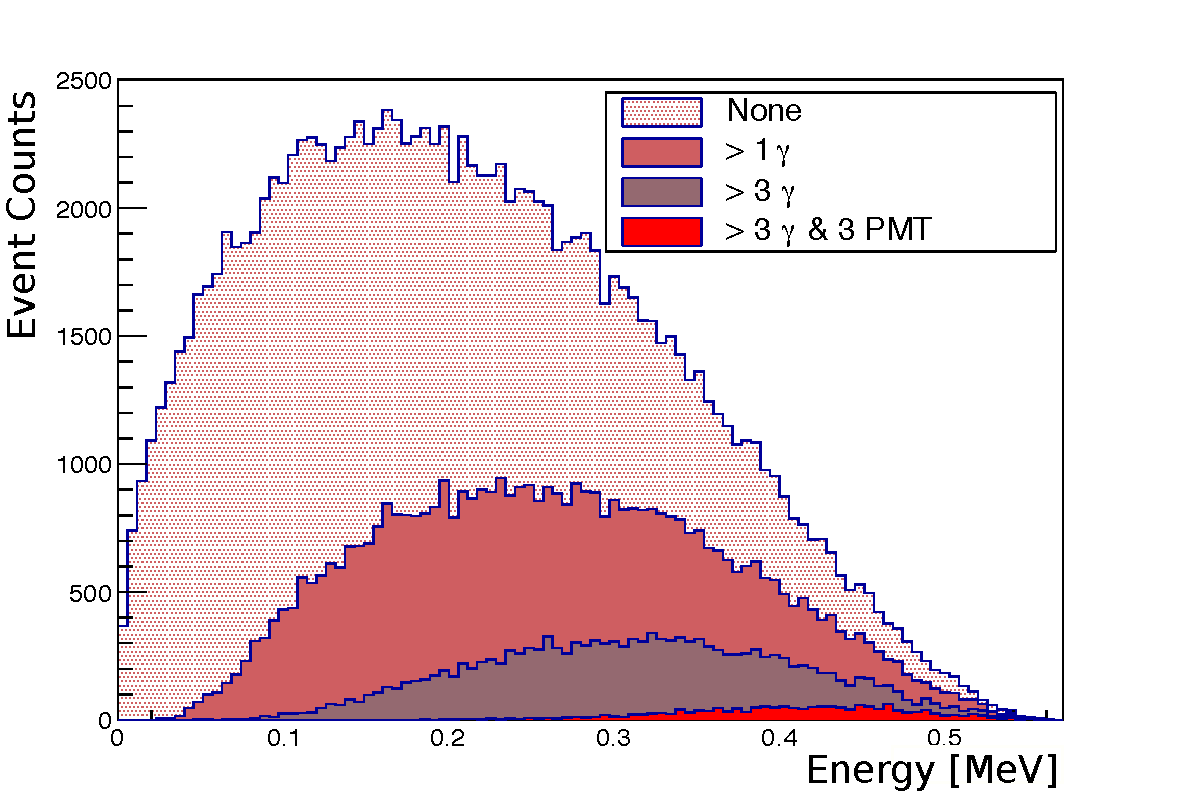
\includegraphics[width=0.45\textwidth]{ar39_energy_spectrum_60pmts_vuv_labels.pdf}
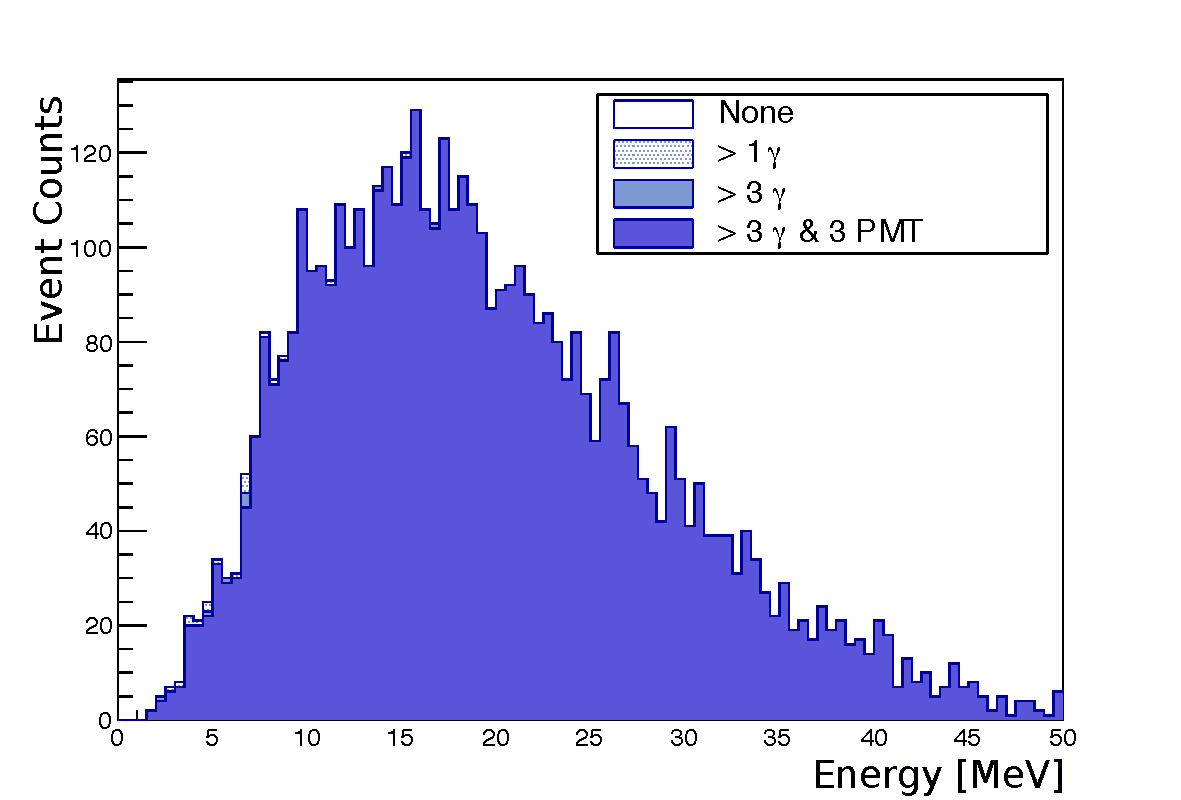
\includegraphics[width=0.45\textwidth]{sn_energy_spectrum_60pmts_vuv_labels.pdf}
\caption{For the no reflective foils configuration - Energy spectra for $^{39}$Ar and supernova neutrinos, assuming a large statistics sample for both, to observe how cuts on the number of photoelectrons per a number of PMTs modify the spectra. The goal for the $^{39}$Ar spectrum is to remove it completely through these cuts, and therefore almost disappears from the plot in the case of the most aggressive cuts. Legend shows cuts where ''1 $\gamma$" corresponds to the cut 1 photoelectron on 1 PMT.}\label{scint_energy_cuts_vuv}
\end{figure}

As the cuts become more stringent, the $^{39}$Ar spectrum almost disappears, while the supernova spectrum is mostly preserved. Additionally, as the cuts require more photoelectrons, intuitively this limits all but the higher energy $^{39}$Ar decays, which occur with a lower frequency. By requiring a signal on several different PMTs, the cuts place a geometry constraint on $^{39}$Ar events occurring in low visibility voxels. Using the same cuts, we can look at the number of PMTs seeing at least one photoelectron per event in Figure \ref{num_pmts}. In a comparison between the two sets of plots: the higher light yield system preserves both the low energy supernova and low energy $^{39}$Ar. However, as also indicated in Table \ref{cuts_table}, the no foils configuration begins to lose efficiency to increase purity. This can be seen in some of the lowest energy supernova events being lost.

Figure \ref{num_pmts} indicates further how the single events are distributed across the PMTs by showing that in the full foils configuration even the lowest energy supernova neutrinos are detected by over half of the PMTs. Conversely a majority of the $^{39}$Ar events are detected on less than half of the PMTs, and when requiring a signal larger than 1 photoelectron on the PMT shrinks exclusively to less than 5 PMTs. This demonstrates how useful making a cut on the number of PMTs in addition to the total number of photoelectrons can be. While the number of different PMTs selected for the cuts (3) is more of a tuning decision, and is investigated further in Section \ref{time_rejection}.

\begin{figure}[H]
\center
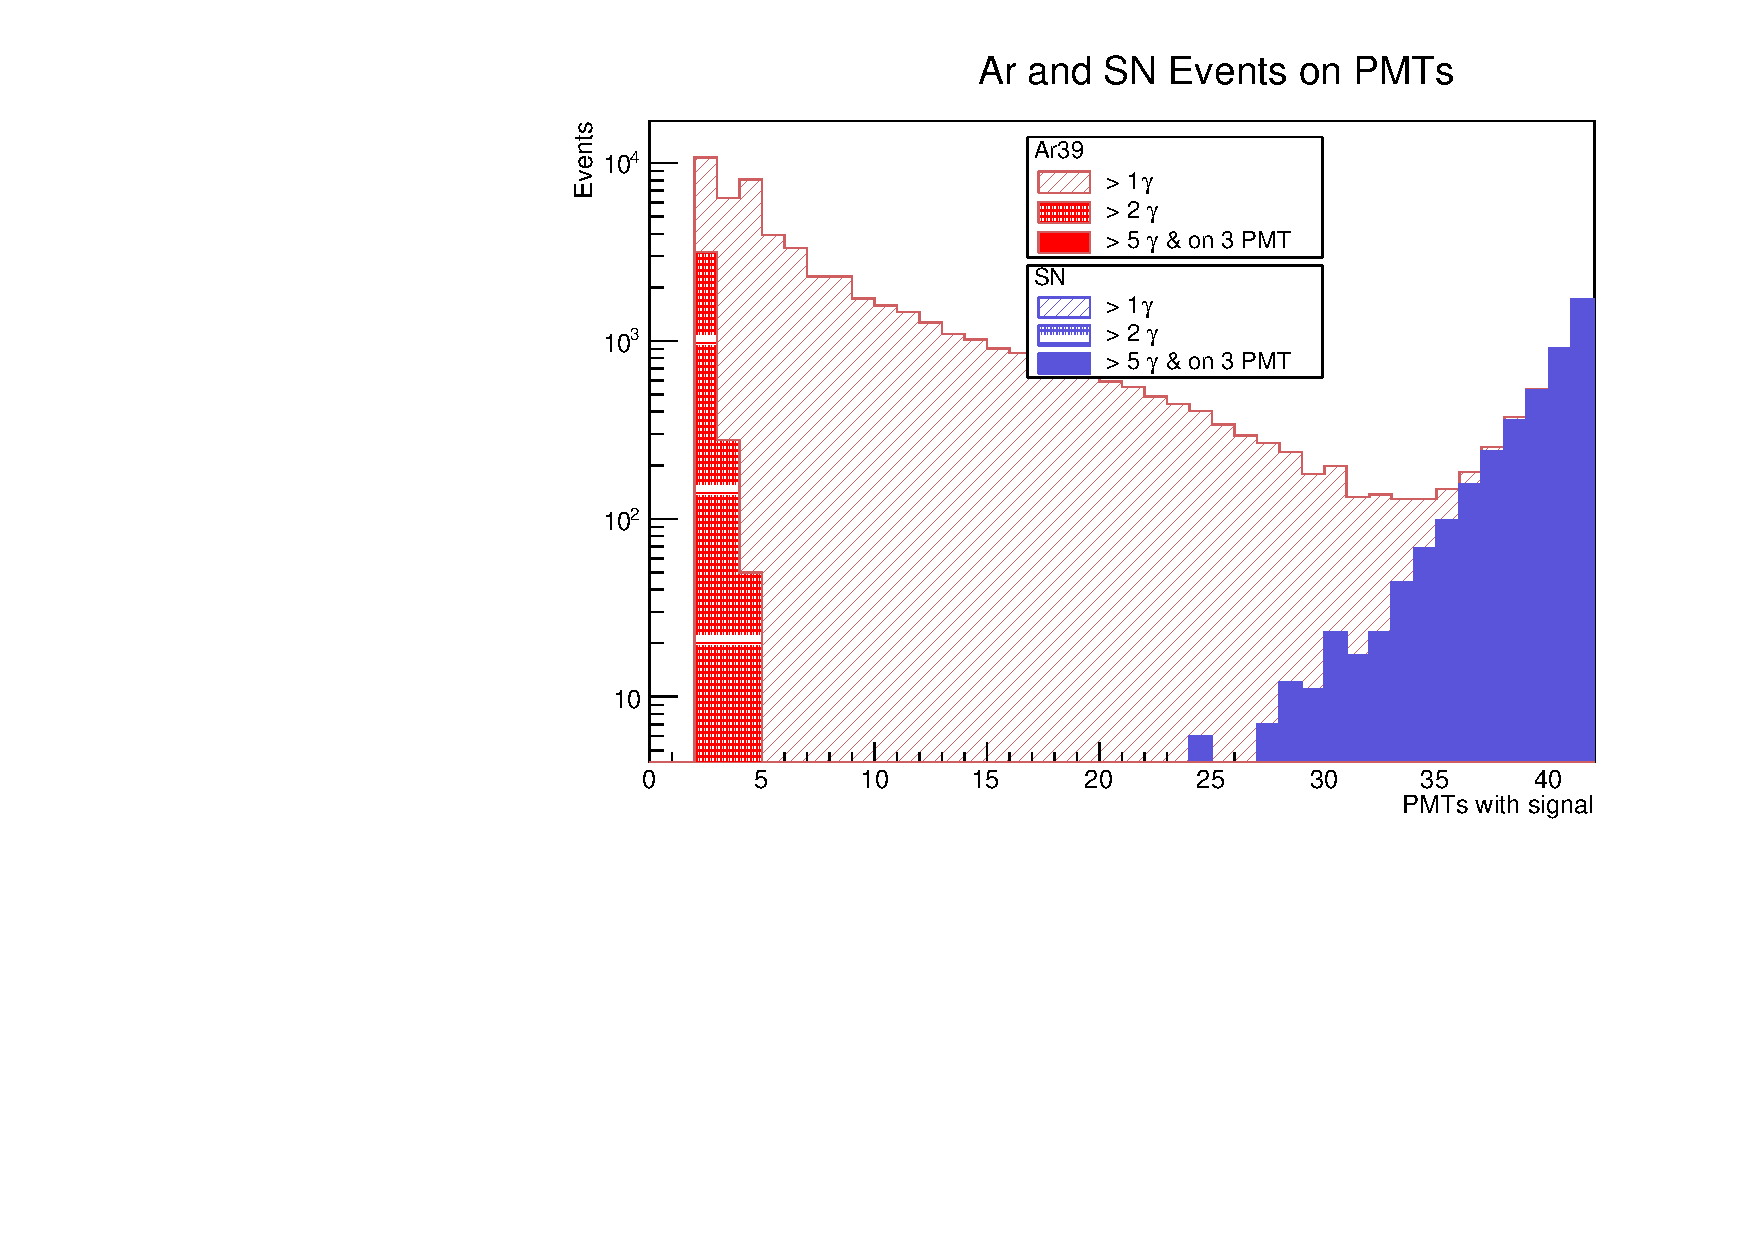
\includegraphics[width=0.45\textwidth]{num_pmts_uniform.pdf}
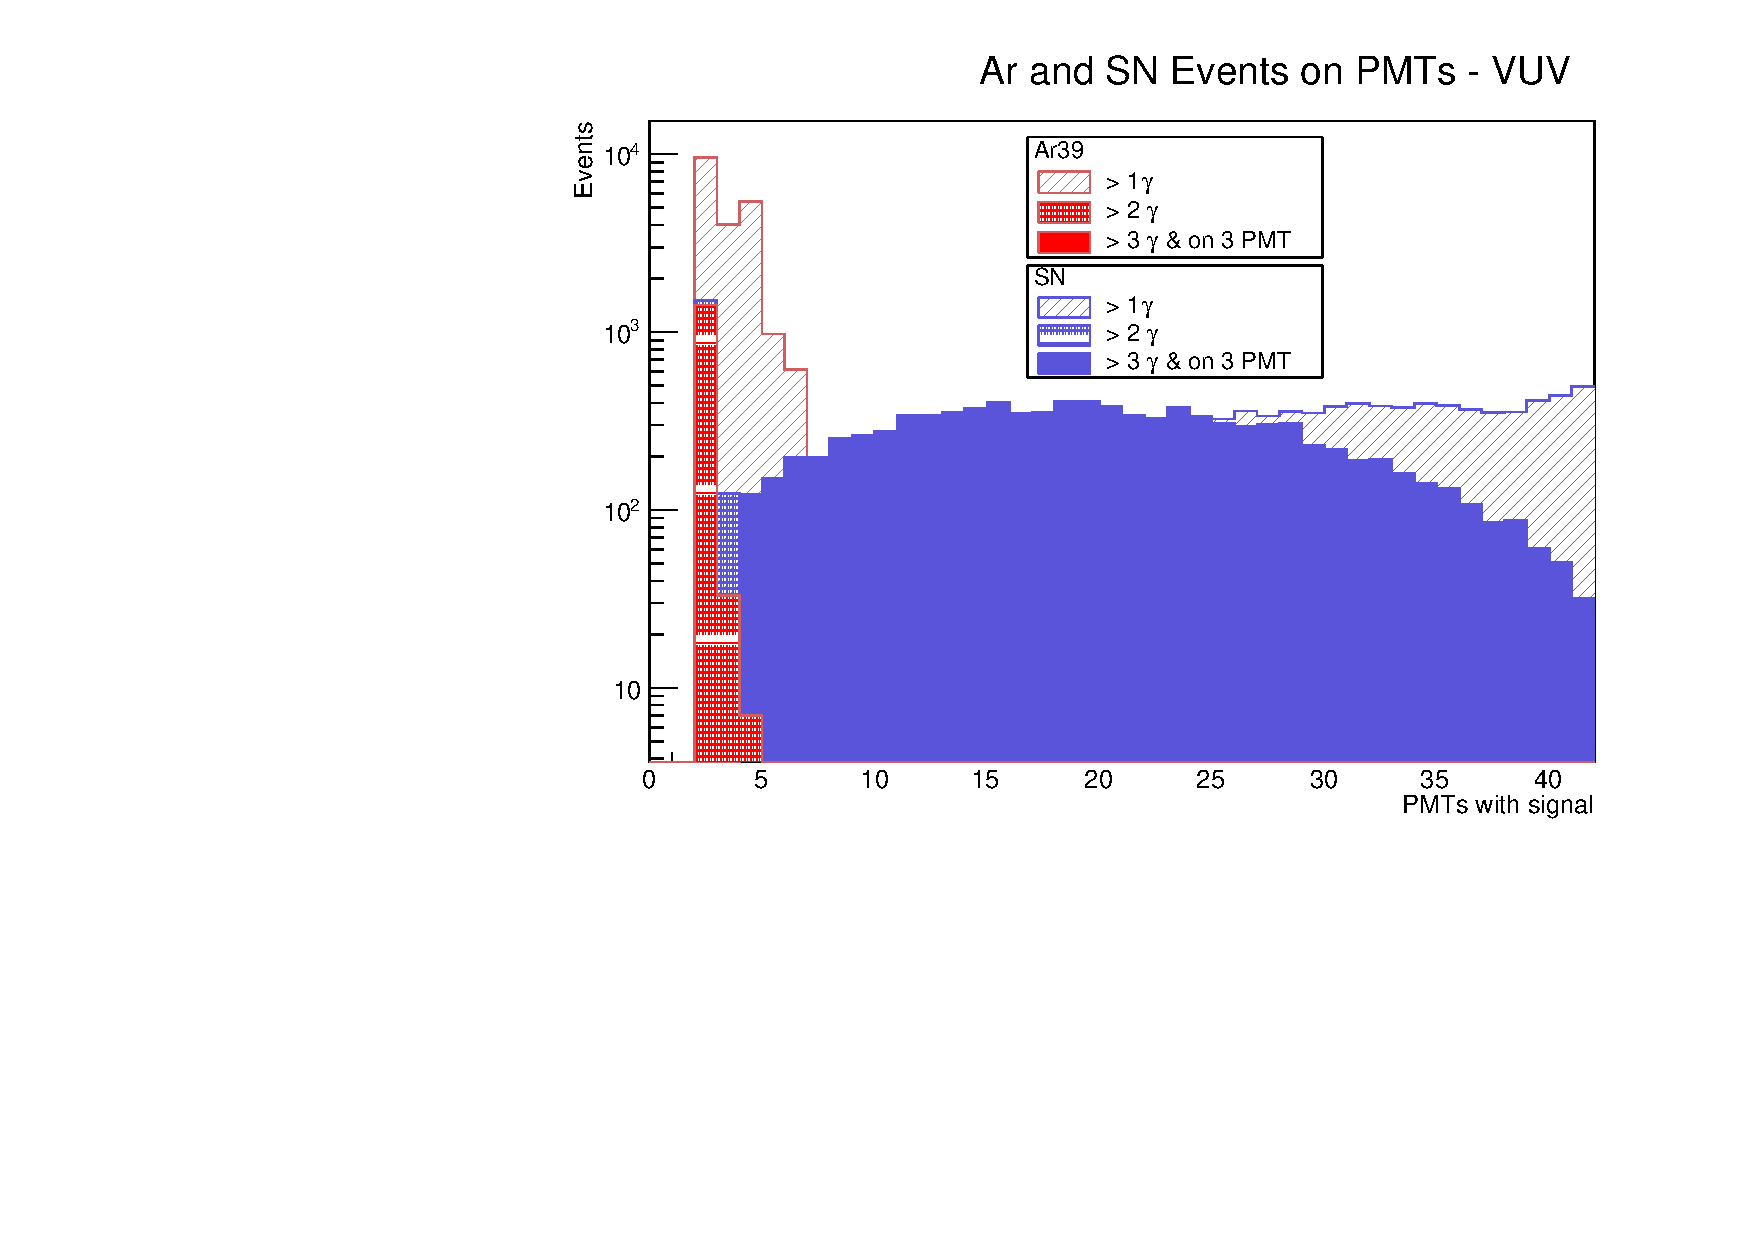
\includegraphics[width=0.45\textwidth]{num_pmts_vuv_only_uniform_adjusted_cuts.pdf}
\caption{Number of PMTs seeing signal for an event, changing based on cuts. Left: supernova spectrum remains unchanged for full foils case, where quickly $^{39}$Ar events become limited to events on fewer than 5 PMTs, and eventually disappear. Right: without reflective-foils, some supernova events move from being visible on all PMTs to being visible on fewer, however all remain above maximum cut of 3 PMTs. Bin 0 has been omitted.}\label{num_pmts}
\end{figure}

As the single $^{39}$Ar event background appears to be removed with rather simple cuts independent of using the reflective-foils, increasing the light generated from the potential supernova neutrino events by including the reflective-foils would result in a majority of supernova events being incident on over 35+ PMTs after cuts, versus 15+. This results in a higher efficiency, however the efficiency without foils is still over 95\%.

\subsection{Single Events - Fast Light Cut}

The single events use the total integrated signal for an event, potentially including photoelectrons generated several microseconds after the first photoelectron was registered on the PMT. This is of course unphysical. As an intermediate solution to gain insight into how the cuts would perform on a more realistic time scale, only the "fast" light of the single events were cut on. In this case, "fast" light is referring to light which is emitted due to the fast scintillation decay and occurs on the scale of 100 nanoseconds. The immediate results of these cuts are visualised on Figure \ref{pmt_maps_fastlight}, where the same events from Figure \ref{pmt_maps} have been reduced to only their fast light component.

\begin{figure}[H]
  \center
      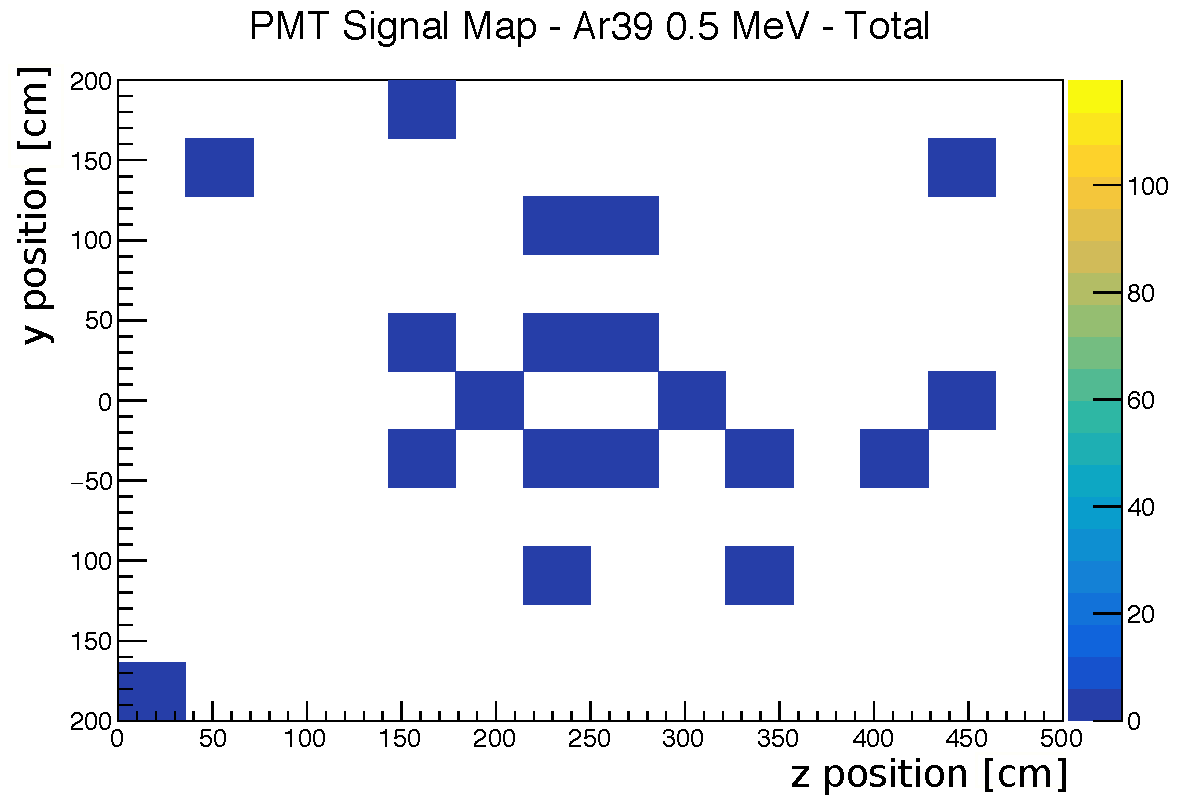
\includegraphics[width=0.43\textwidth]{ar39_signal_map_improved_fastlight_2_labels.pdf}
      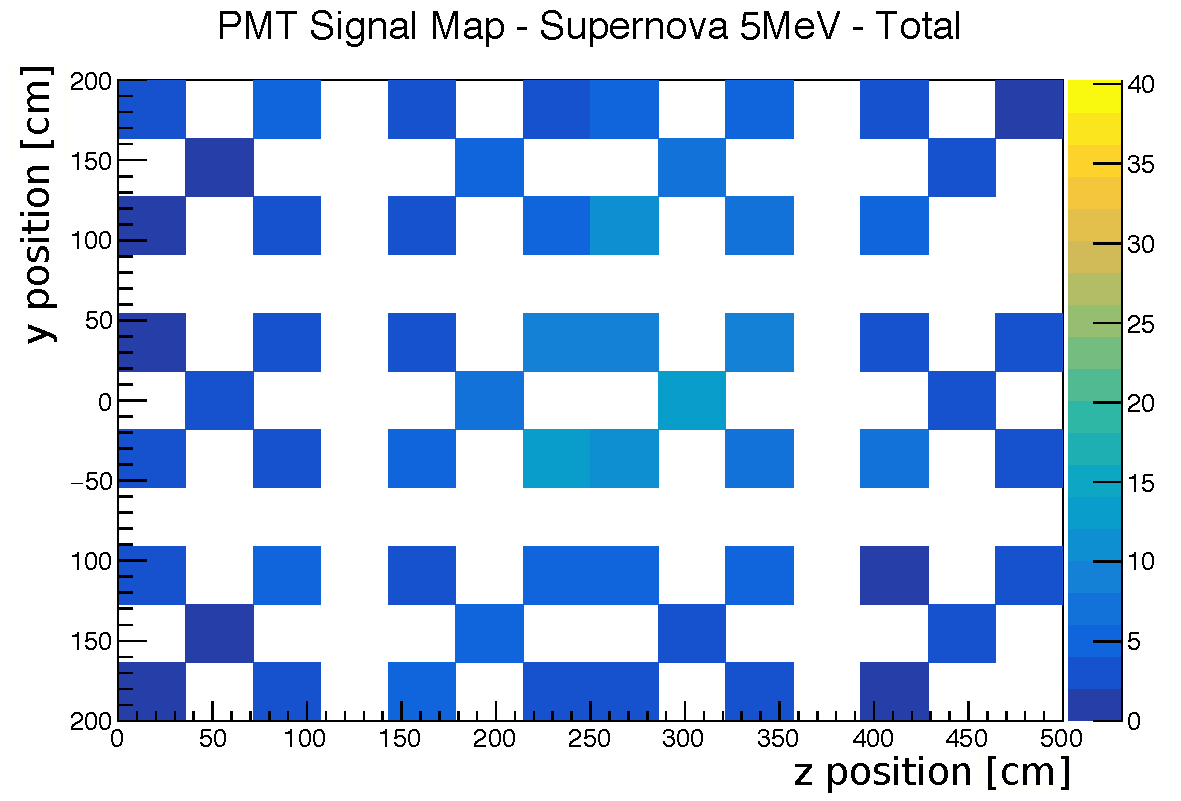
\includegraphics[width=0.43\textwidth]{sn_signal_map_improved_fastlight_labels.pdf}
      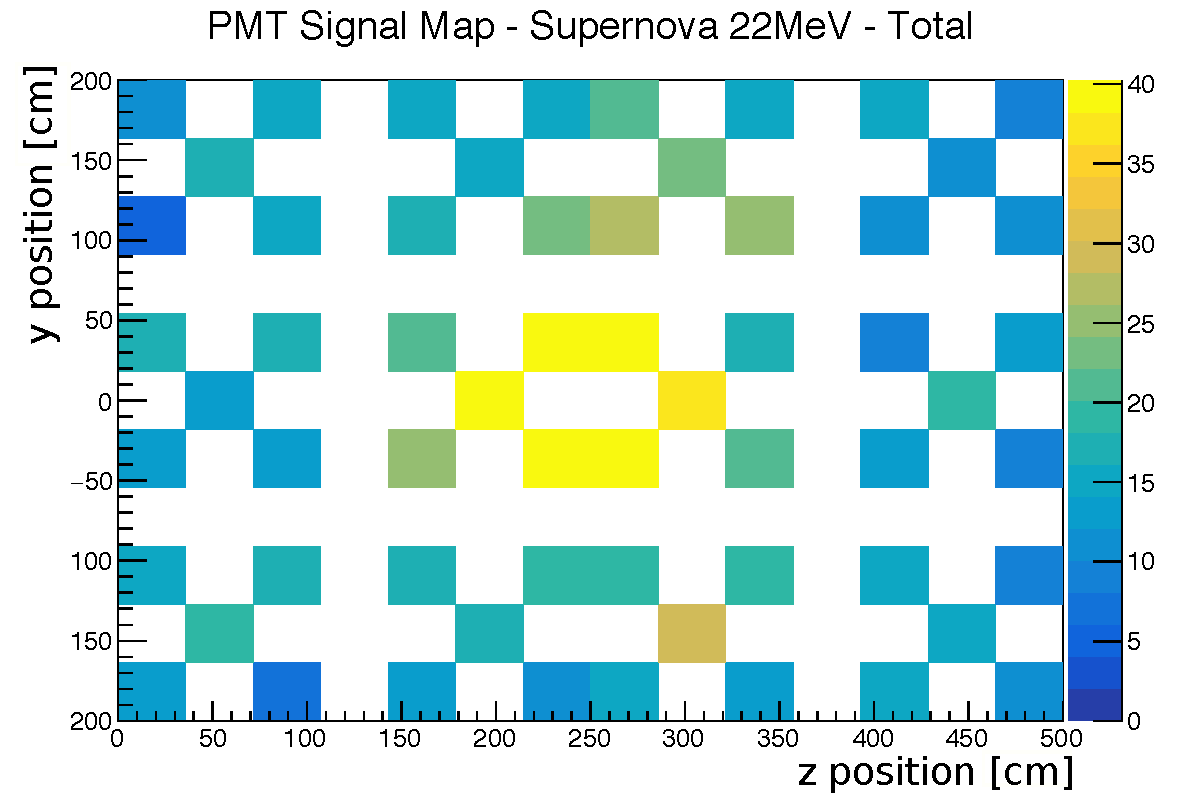
\includegraphics[width=0.43\textwidth]{sn_signal_map_higherE_improved_fastlight_labels.pdf}
      \caption{Comparison of single high-energy $^{39}$Ar, 5 MeV SN, and 22 MeV SN events in middle of detector using 60 PMTs. This is for the "fast" light case, where the number of photoelectrons is cut by rougly 75\%. Shown are the results for the total light (VUV+visible) in the case of full reflective foils. Color (z-axis) corresponds to number of photoelectons.}\label{pmt_maps_fastlight}
\end{figure}

Examining only the single $^{39}$Ar decay, taking the light emitted in the first 100 nanoseconds only seems to effectively reduce the number of PMTs seeing signal by about 25\%. From this result, we would largely expect the required cut on the photoelectrons to go down, as the cut on multiple PMTs becomes more effective and the total signal accepted per event is decreased. Table \ref{cuts_table_fastlight} shows the updated cuts and efficiencies when considering only the fast light.

\begin{table}[H]
	\begin{center}
	\begin{tabular}{| c | c || c | c ||}
	\hline
	No. PE & No. PMT & $\%$ $^{39}$Ar & $\%$ $^{39}$Ar VUV\\
	\hline
	 & & &\\
	 1 & 1 & 60.2  & 84.5\\
	 & & &\\
	 2 & 1 & 97.3 & 98.8\\
	 & & &\\
	 2 & 2 & 73.7 & 93.2\\
	  & & &\\
	 3 & 2 & 97.4 & 99.9\\
	 & & &\\
	 3 & 3 &  98.0 & 99.9\\
	 & & &\\
	 3 & 4 & 99.2 & X\\
	 & & &\\
	 4 & 2 & 99.8 & X\\
	 & & &\\
	 4 & 3 & 99.8 & X\\
	 & & &\\
	 5 & 3 & 99.9 & X\\
	\hline
	\end{tabular}
	\end{center}
	\caption{\% Reduction in signal and background compared for the reflective foil and no reflective foils configurations, when considering the fast light. ``VUV'' indicates the no reflective foil case and ``X'' indicates that the cut is not relevant for this case.}\label{cuts_table_fastlight}
	\end{table}
	
As before, the cuts were used as guidance to show the reductions of the energy spectra for $^{39}$Ar as well as the supernova events, for both the full foil and no foil (vuv only) cases. These are shown as Figures \ref{scint_energy_cuts_fastlight} and \ref{scint_energy_cuts_vuv_fastlight} respectively. The events appear to behave as expected - lower light yield means lower trigger rate. However the lower light yield also resulted in some losses to the supernova neutrino signal.

\begin{figure}[H]
\center
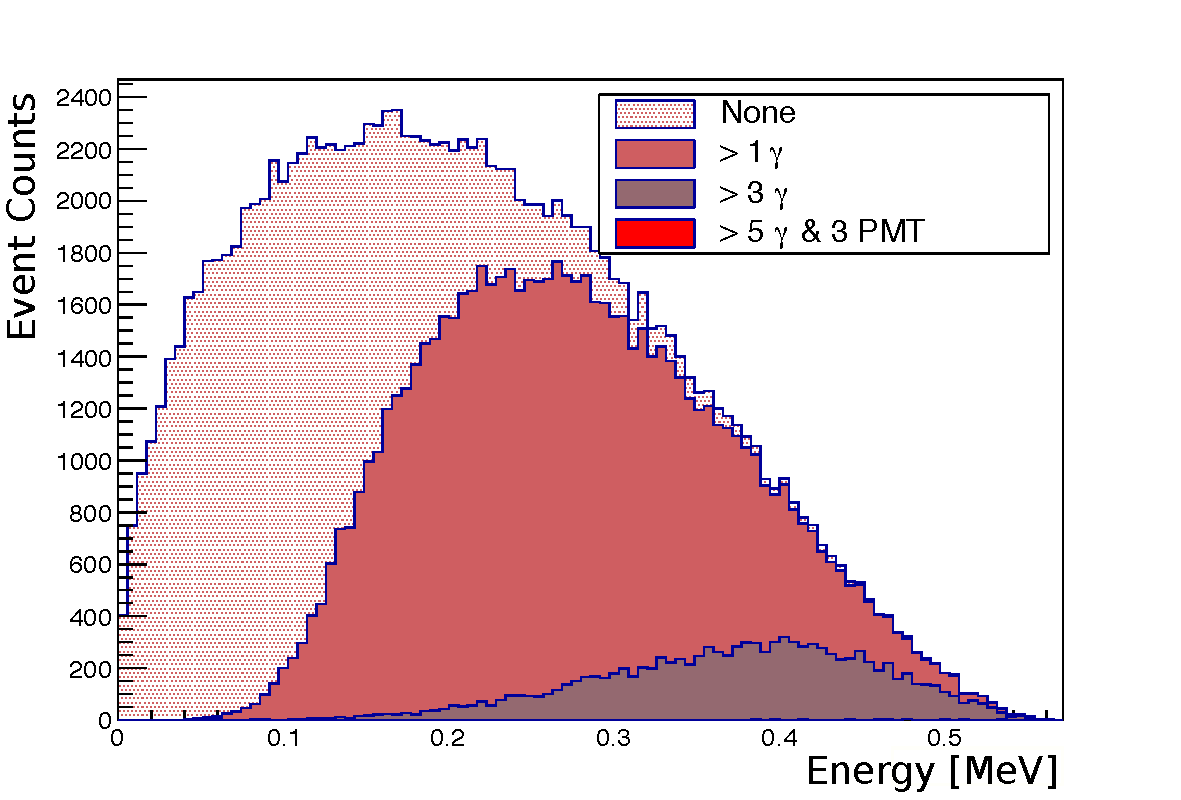
\includegraphics[width=0.45\textwidth]{ar39_energy_spectrum_60pmts_fastlight_labels.pdf}
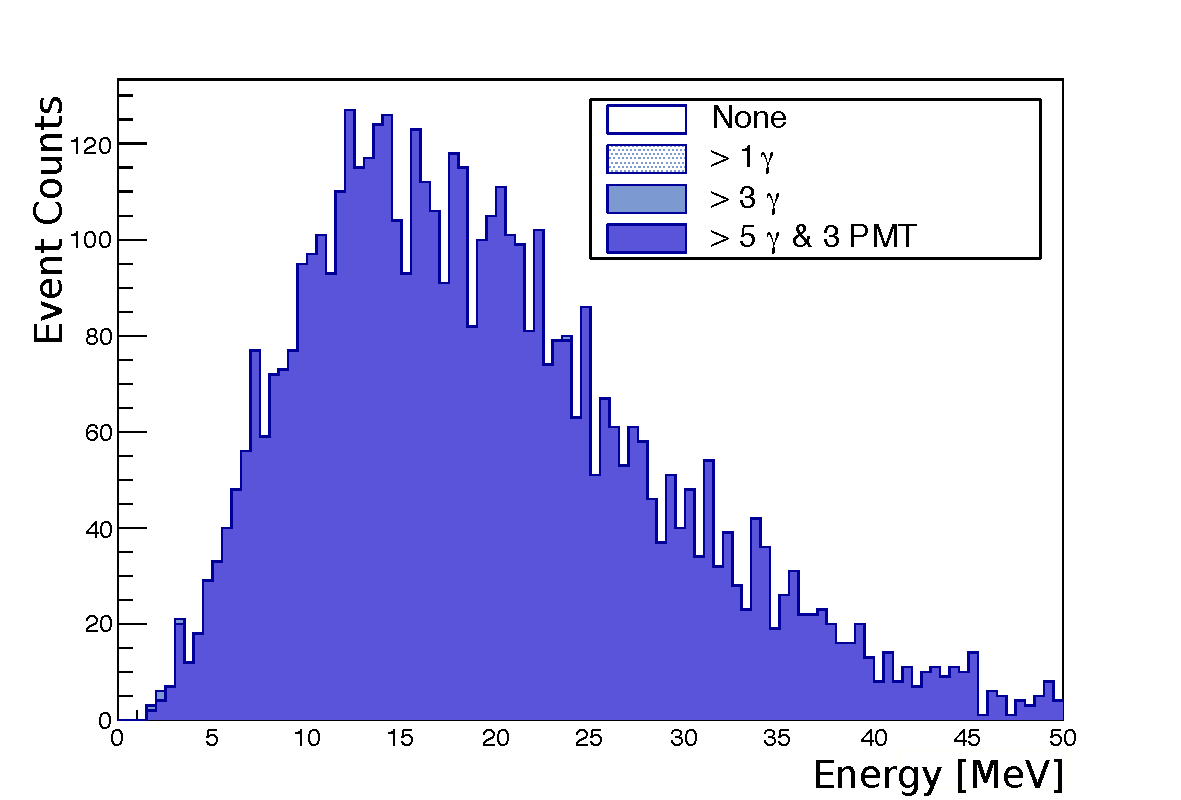
\includegraphics[width=0.45\textwidth]{sn_energy_spectrum_60pmts_fastlight_labels.pdf}
\caption{Energy spectra for $^{39}$Ar and supernova neutrinos, assuming a large statistics sample for both, to observe how cuts on the number of photoelectrons per a number of PMTs modify the spectra. This case assumes reflective foils, considers the contribution from both direct VUV and reflected visible light, and replicates measuring only the ``fast" light component by accepting only photoelectrons measured in the first 100 nanoseconds. The goal for the $^{39}$Ar spectrum is to remove it completely through these cuts, and therefore disappears from the plot in the case of the most aggressive cuts. }\label{scint_energy_cuts_fastlight}
\end{figure}

\begin{figure}[H]
\center
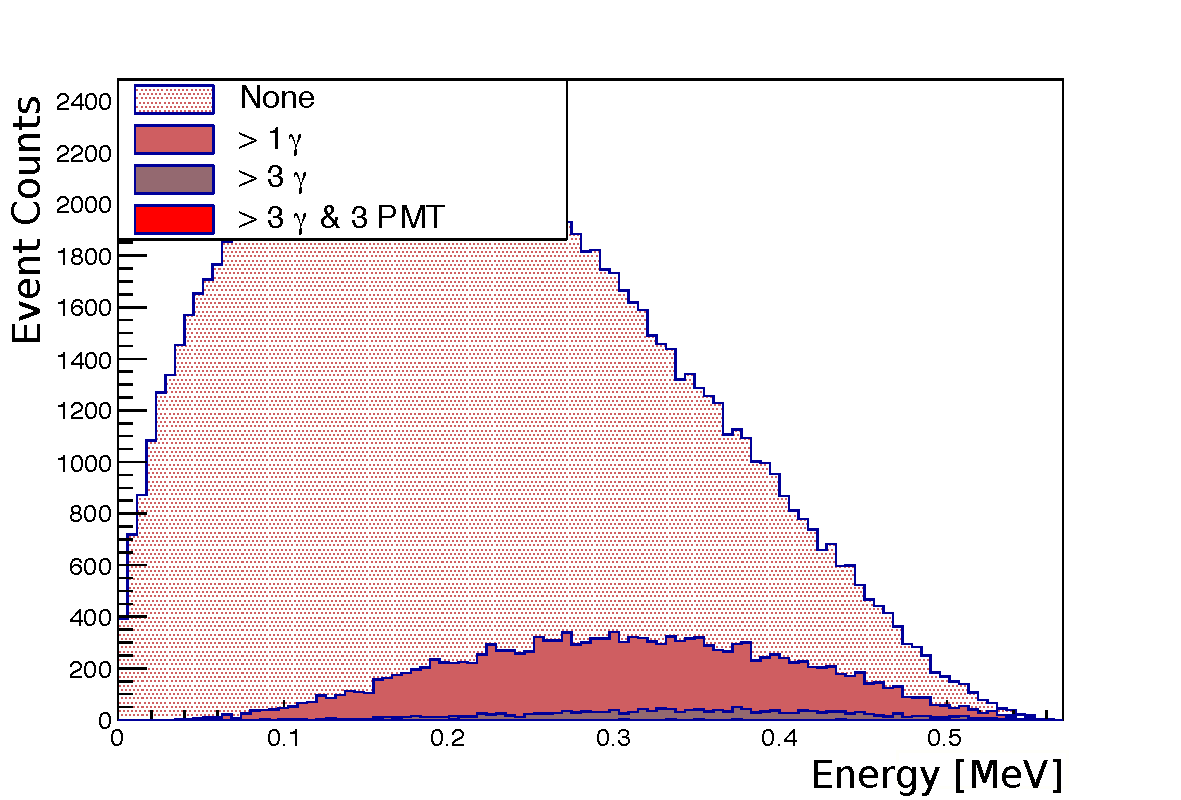
\includegraphics[width=0.45\textwidth]{ar39_energy_spectrum_60pmts_vuv_fastlight_labels.pdf}
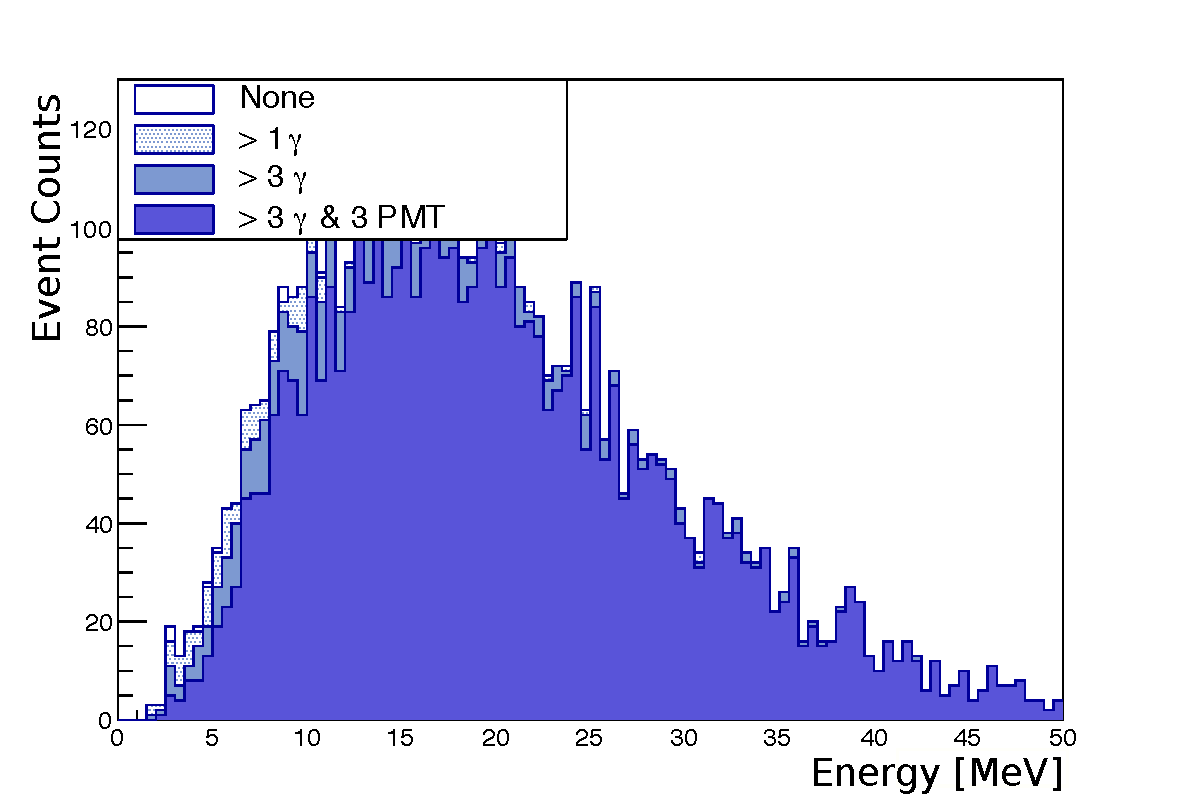
\includegraphics[width=0.45\textwidth]{sn_energy_spectrum_60pmts_vuv_fastlight_labels.pdf}
\caption{Energy spectra for $^{39}$Ar and supernova neutrinos, assuming a large statistics sample for both, to observe how cuts on the number of photoelectrons per a number of PMTs modify the spectra. The goal is to completely remove the $^{39}$Ar spectrum through these cuts. This is for the no reflective foils configuration and accepts only the first 100 nanoseconds, to replicate measuring only the ``fast" light component.}\label{scint_energy_cuts_vuv_fastlight}
\end{figure}

Although the method of considering the fast light makes a step towards a more physical description of the system, the decays happen constantly. Considering decays on a purely event-wise basis excludes the possibility for photoelectrons from two or more $^{39}$Ar decays to occur on the same PMT at the same time. Such exclusion allows for the interesting comparison of the background and signal energy spectra, however by allowing the photoelectrons from different decays to "interfere", the system is more accurately described. 

\subsection{Time Rejection}\label{time_rejection}

Single events provide a convenient insight into an expected large sample, however signals from multiple events close in time may lead to enhanced rates of $^{39}$Ar passing the cuts. However, as the cuts from Table \ref{cuts_table} and \ref{cuts_table_fastlight} were rather simple, the idea behind them is carried forward to a slightly more advanced trigger. Some comments about realistic trigger configurations are made in Section \ref{ar39_conclusion}.

Based on Figure \ref{pmts_time}, multiple background decays close in time are capable of causing a trigger when using cuts designed for single events. To prevent this, the trigger should include some timing window during which the threshold must be reached. We have seen in the fast-light only results, that the supernova neutrino events produce sufficient fast light to trigger the system in this way. For example the trigger can be constructed now with two steps. The first step being a check of several PMTs seeing a signal within a small amount of time. If this is fulfilled then a second, longer time window is opened to check for additional photons on each of those PMTs. The number of photons here is adjusted like in the single event cuts. The number of unique PMTs seeing a signal must occur within 10 ns and each PMTs threshold met or exceeded within 100 ns. Both parameters were varied to find optimal configurations, where the $^{39}$Ar trigger rate is lowest. Because photoelectrons are not tied specifically to an event, the efficiency of rejection is expressed as a rate - the frequency with which $^{39}$Ar decays successfully exceed the thresholds set. The supernova events continue to be considered individually and expressed as an efficiency. Note that after a trigger, the system cannot trigger again until the 100 nanoseconds window for the previous trigger closes.

The performance of the cuts for different LDS configurations are shown in Figure \ref{ar39_cut_maps}, where the colour indicates the intensity of the signal and white bins mean these cut configurations have been excluded or not tested.

\begin{figure}[H]
  \center
      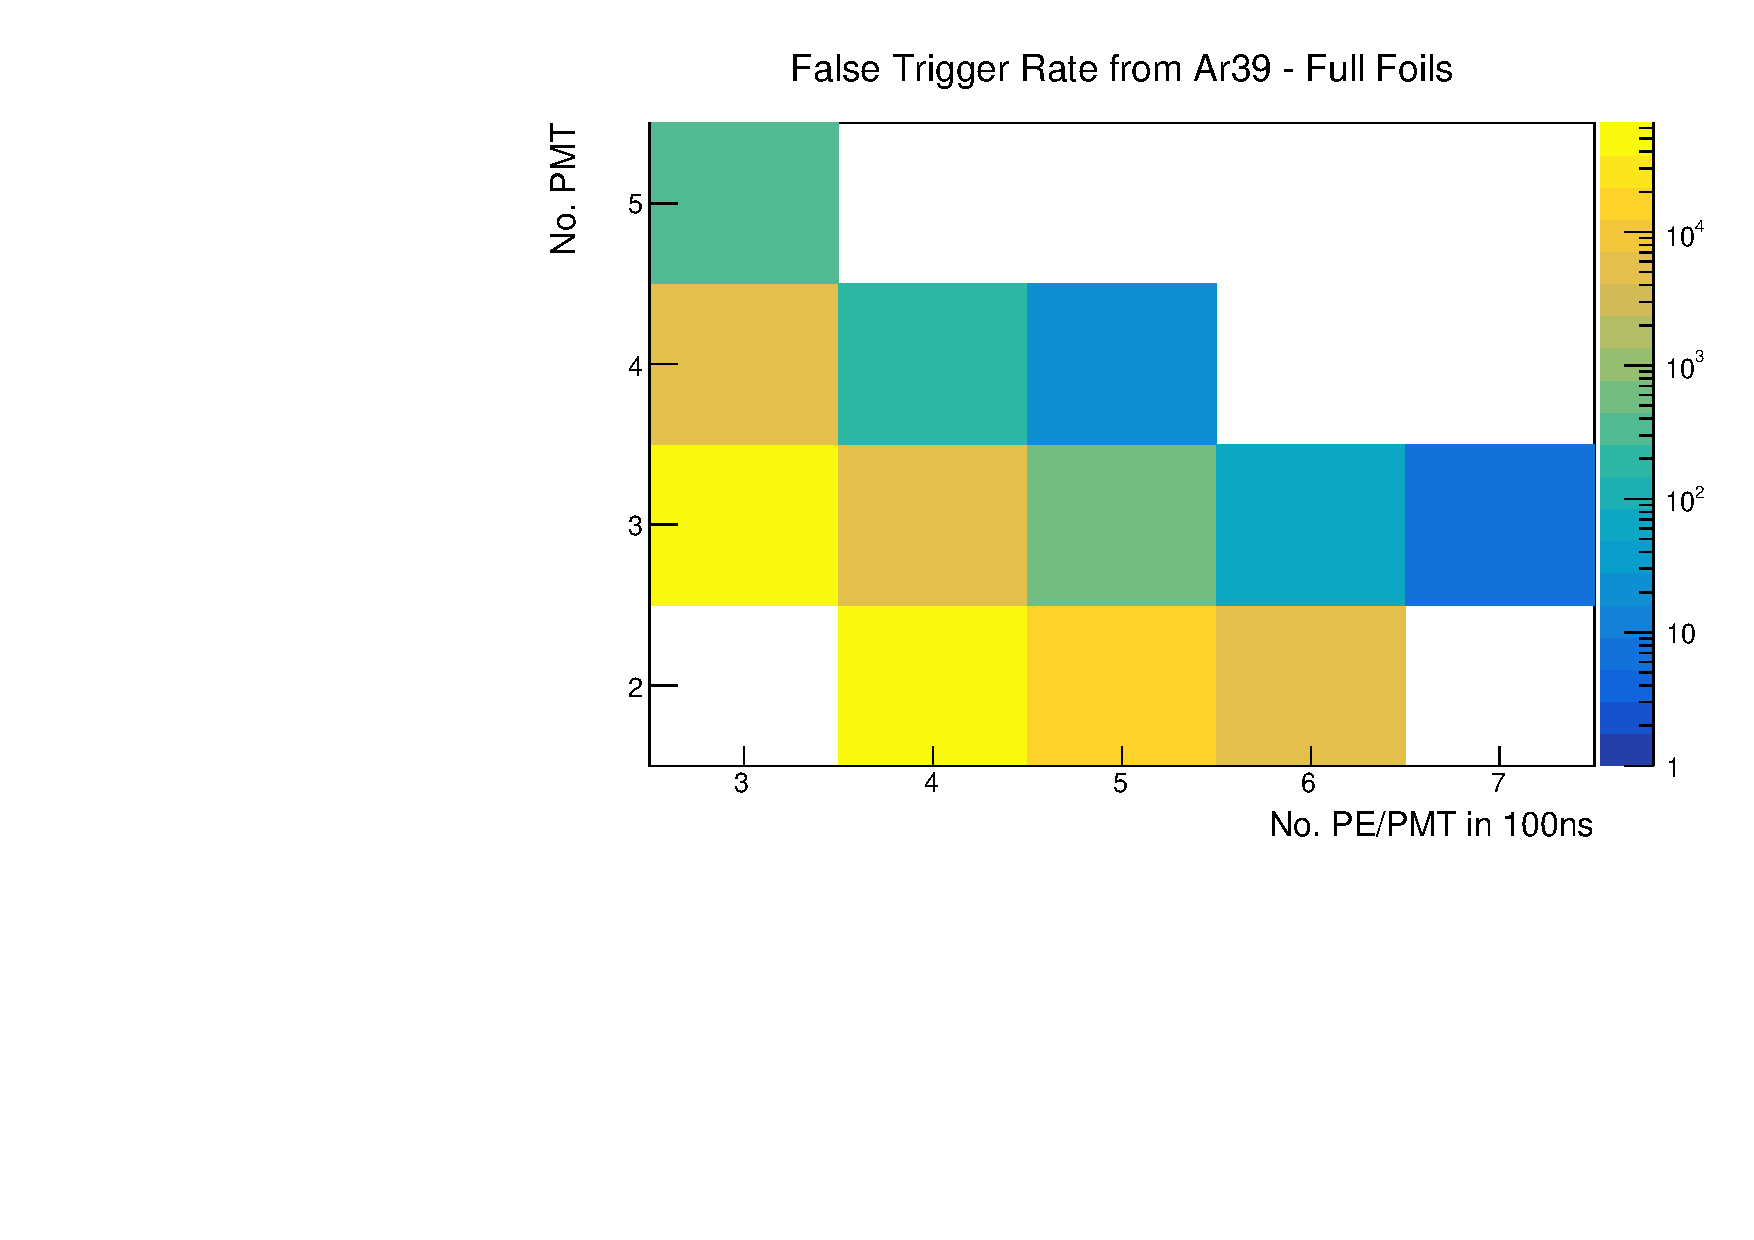
\includegraphics[width=0.43\textwidth]{ar39_trigger_map_fullfoils.pdf}
      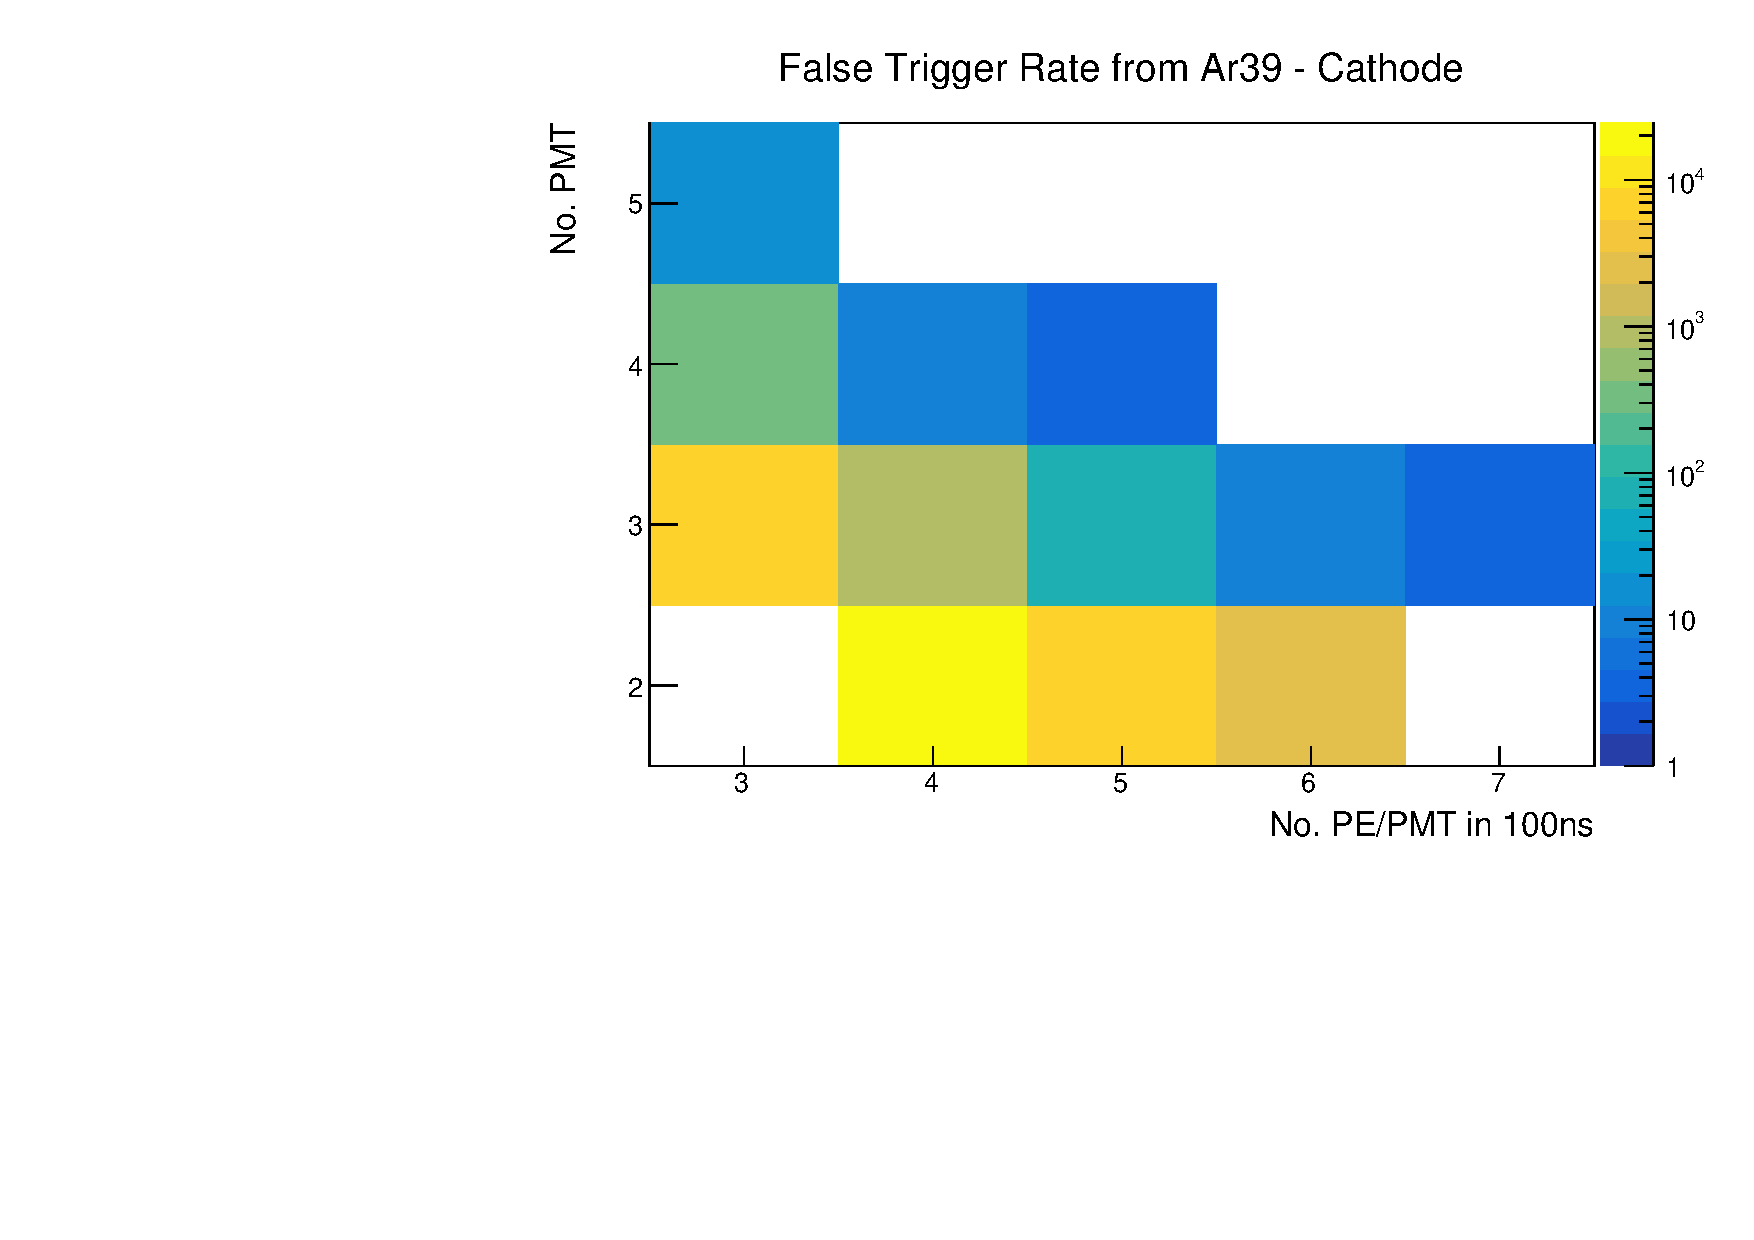
\includegraphics[width=0.43\textwidth]{ar39_trigger_map_cathode.pdf}
      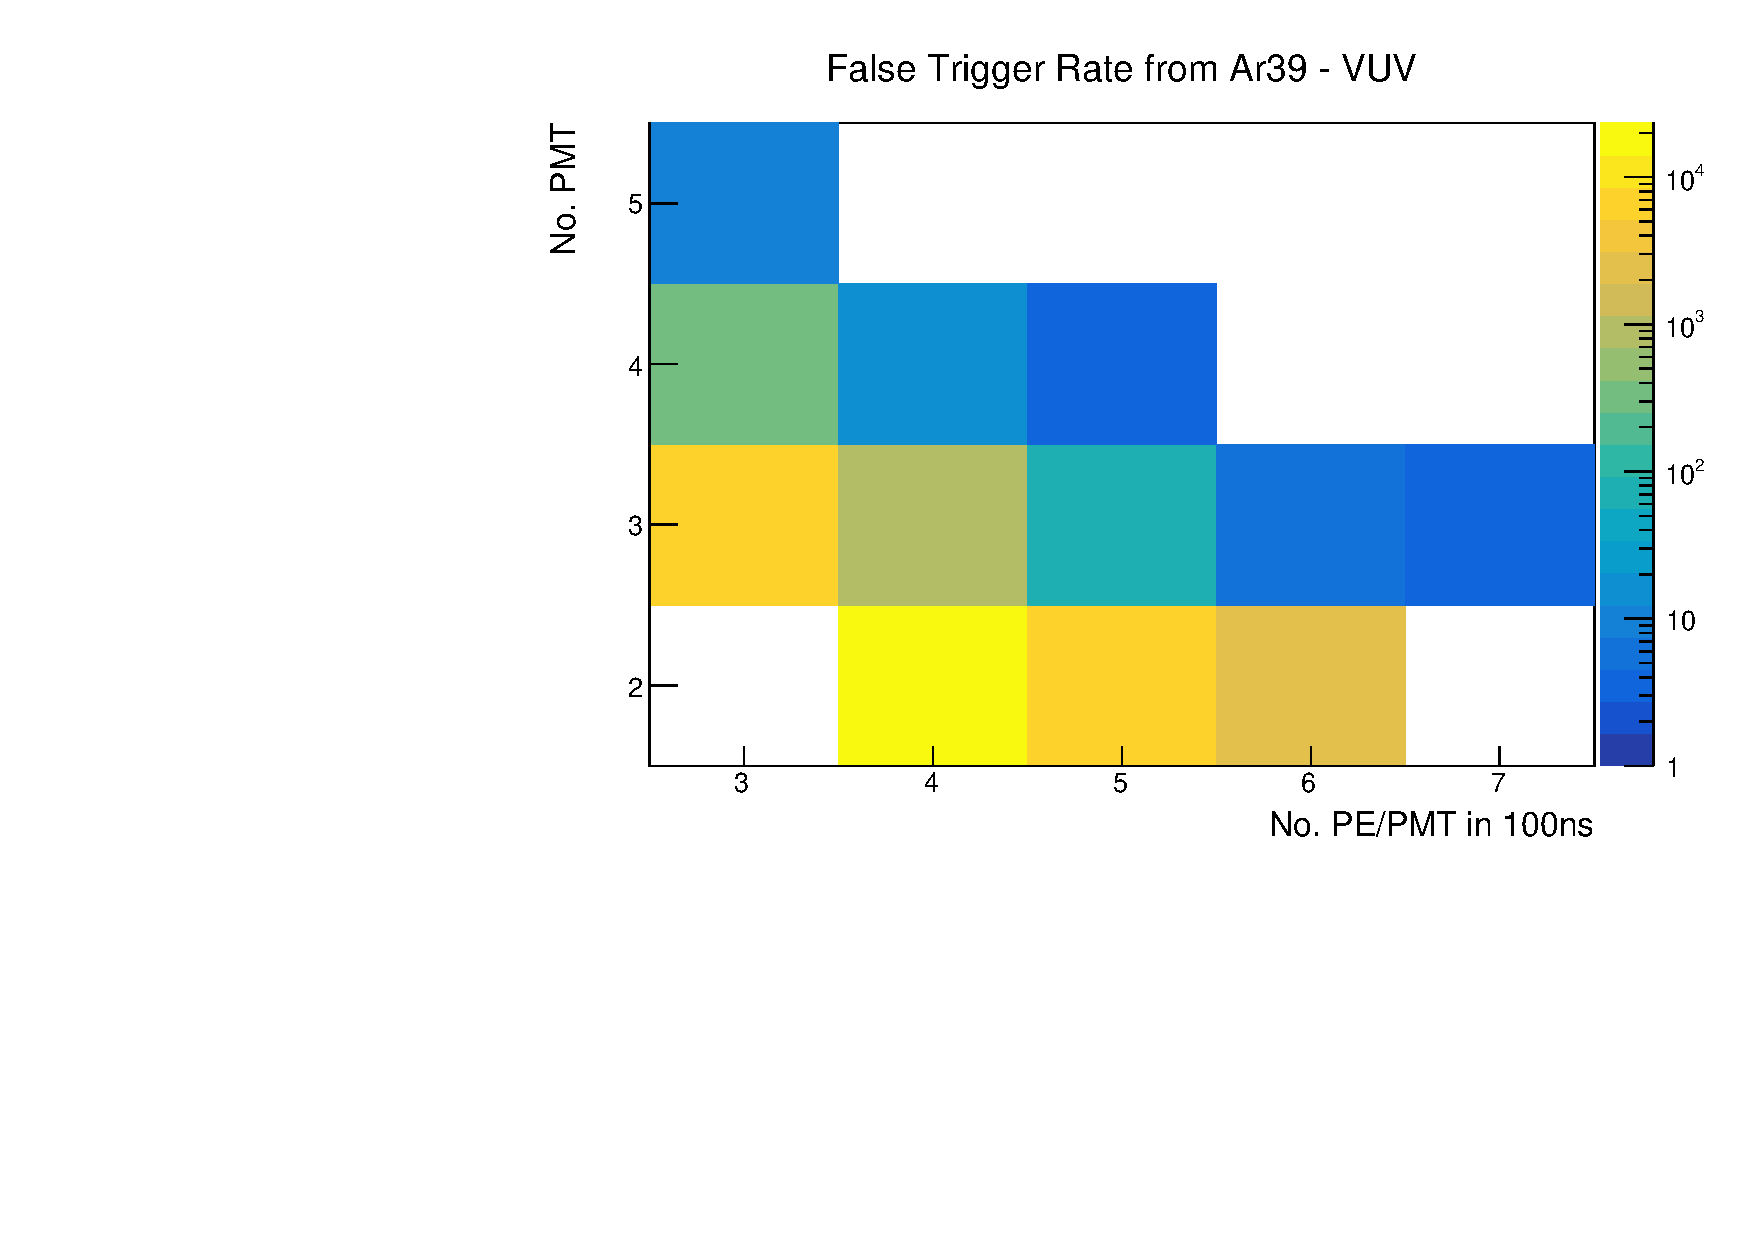
\includegraphics[width=0.43\textwidth]{ar39_trigger_map_vuv.pdf}
      \caption{Comparison of effective cuts to reduce $^{39}$Ar trigger rate for different LDS configurations. The colour indicates the rate of triggers, and as such should be minimised. Therefore in this case, the most effective cuts are identified by the bins with the lowest value (most blue). Note that the plots are not normalised to one another.}\label{ar39_cut_maps} %Plots not normalised as this completely removes some ability to distinguish bin-by-bin information
\end{figure}

Figure \ref{ar39_cut_maps} shows how simple cuts are able to reduce the background signal with timing included, however the threshold has increased from the single event case. Uniform scaling is not applied across the three plots, as the large range makes distinguishing different colours more difficult. For this reason, attention should be given to the scales to the rights of the plots. The representation shown in Figure \ref{false_triggers} allows the different LDS configurations to be compared more easily for a given number of PMTs in 10 nanoseconds. The errors considered here are purely statistical, as the data sample generated creates over $3 \times 10^{6}$ $^{39}$Ar decays, properly sampling the energy distribution, as well as the 320,000 voxels of the detector.

\begin{figure}[H]
\center
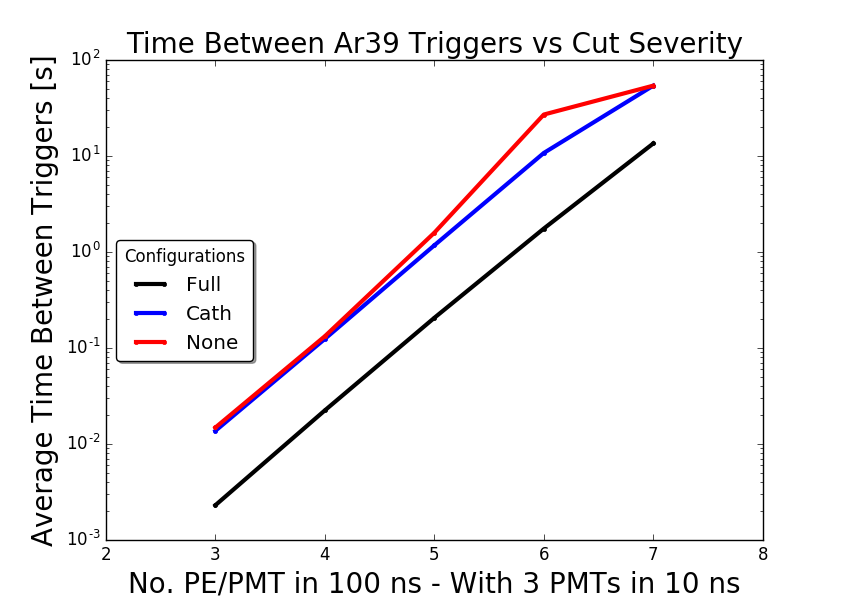
\includegraphics[width=0.5\textwidth]{updated_efficiency_logy_labels.png}
\caption{Average time between triggers due to $^{39}$Ar photoelectrons as a function of the number of the individual PMT thresholds. The plot shows the rejection ability and optimum threshold for three different light system configurations given a requirement of 3 different PMTs in 10 nanoseconds.}\label{false_triggers}
\end{figure}

%In the case of the full foil configuration, the light yield of the system is considerably higher, such that 78\% more light is detected than the cathode case and the reflected light contributes to the closely concentrated VUV signal, resulting in a higher trigger rate. The cathode case has roughly 20\% more light than the no foils case, with much of its light arriving to the PMTs as visible light. This visible light was wavelength shifted by the foils on the cathode and delayed in time compared to the VUV light due to propagation timings (reemission delays are not considered). Both the cathode foil and no foil sets have a majority of the light arriving close in time to each other as the timing spread in VUV light is small. As the thresholds increase, both backgrounds approach zero, as the VUV light is also excluded. 

One of the strictest elements of the cuts are that multiple PMTs need to see a photoelectron within 10 nanoseconds of each other. By increasing the time from 10 to 100 nanoseconds we expect more $^{39}$Ar events to pass the cuts, but also potentially allows the later-arriving visible light to contribute more. Indeed in Figure \ref{ar39_cut_maps_100ns} we see that the overall rates have increased for most of the cut configurations, however the higher threshold values selected before continue to remove the background to rates below 1 Hz.

\begin{figure}[H]
\center
      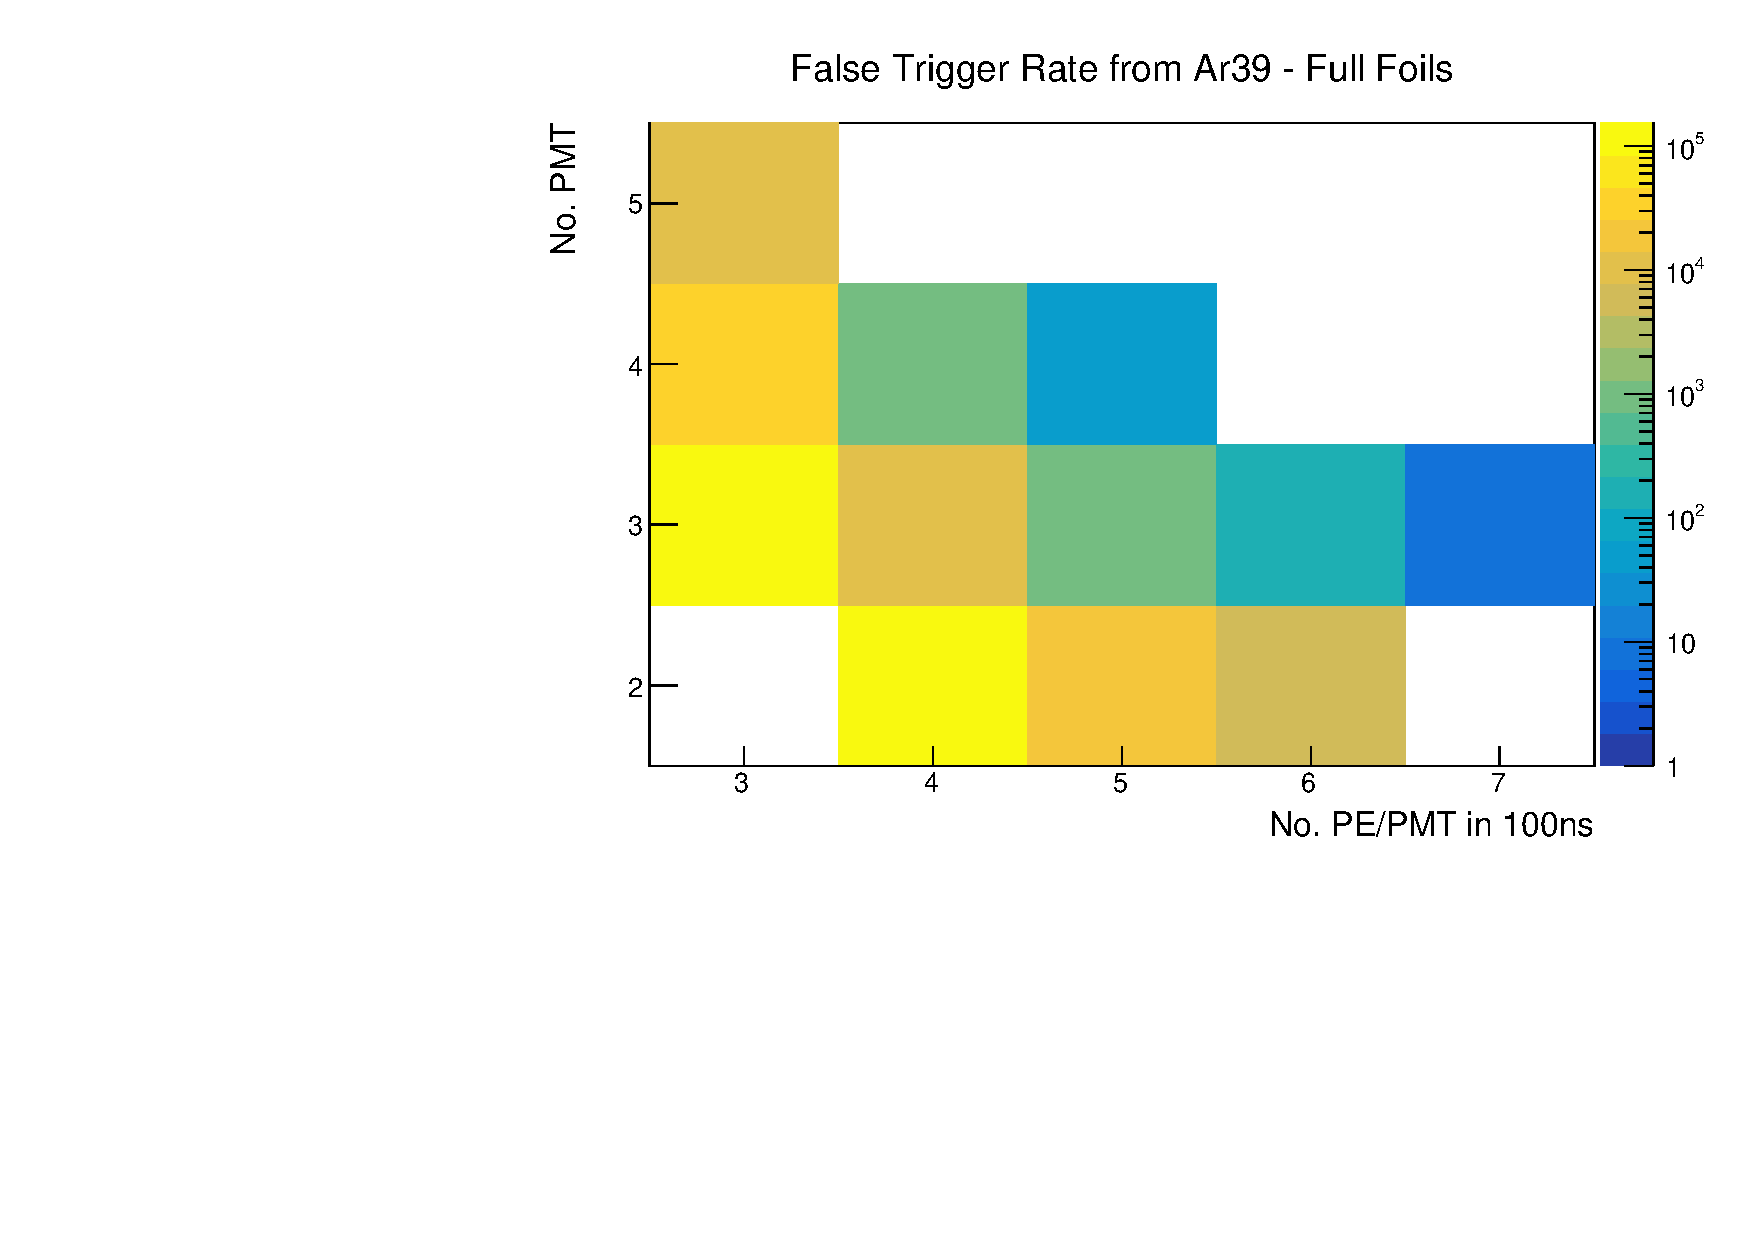
\includegraphics[width=0.43\textwidth]{trigger_map_100_fullfoils.pdf}
      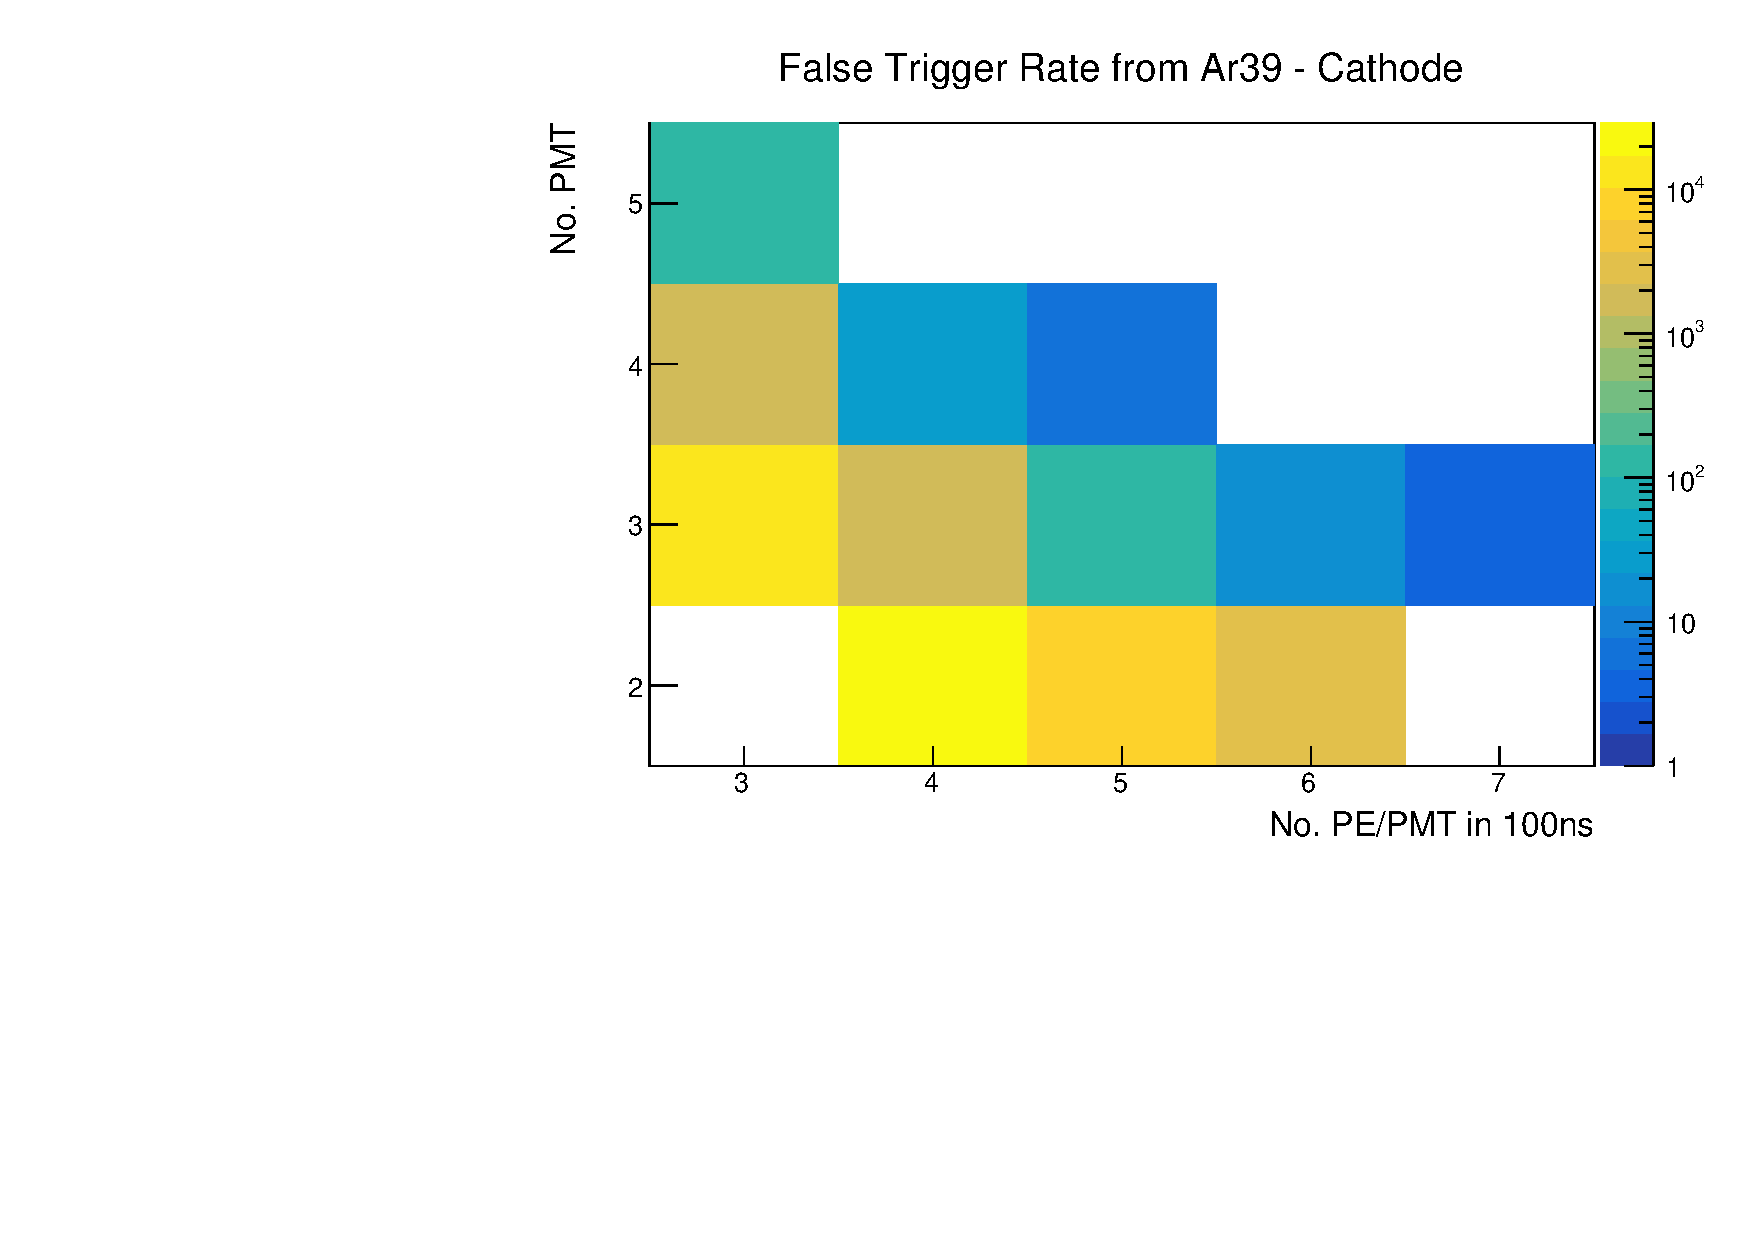
\includegraphics[width=0.43\textwidth]{trigger_map_100_cathode.pdf}
      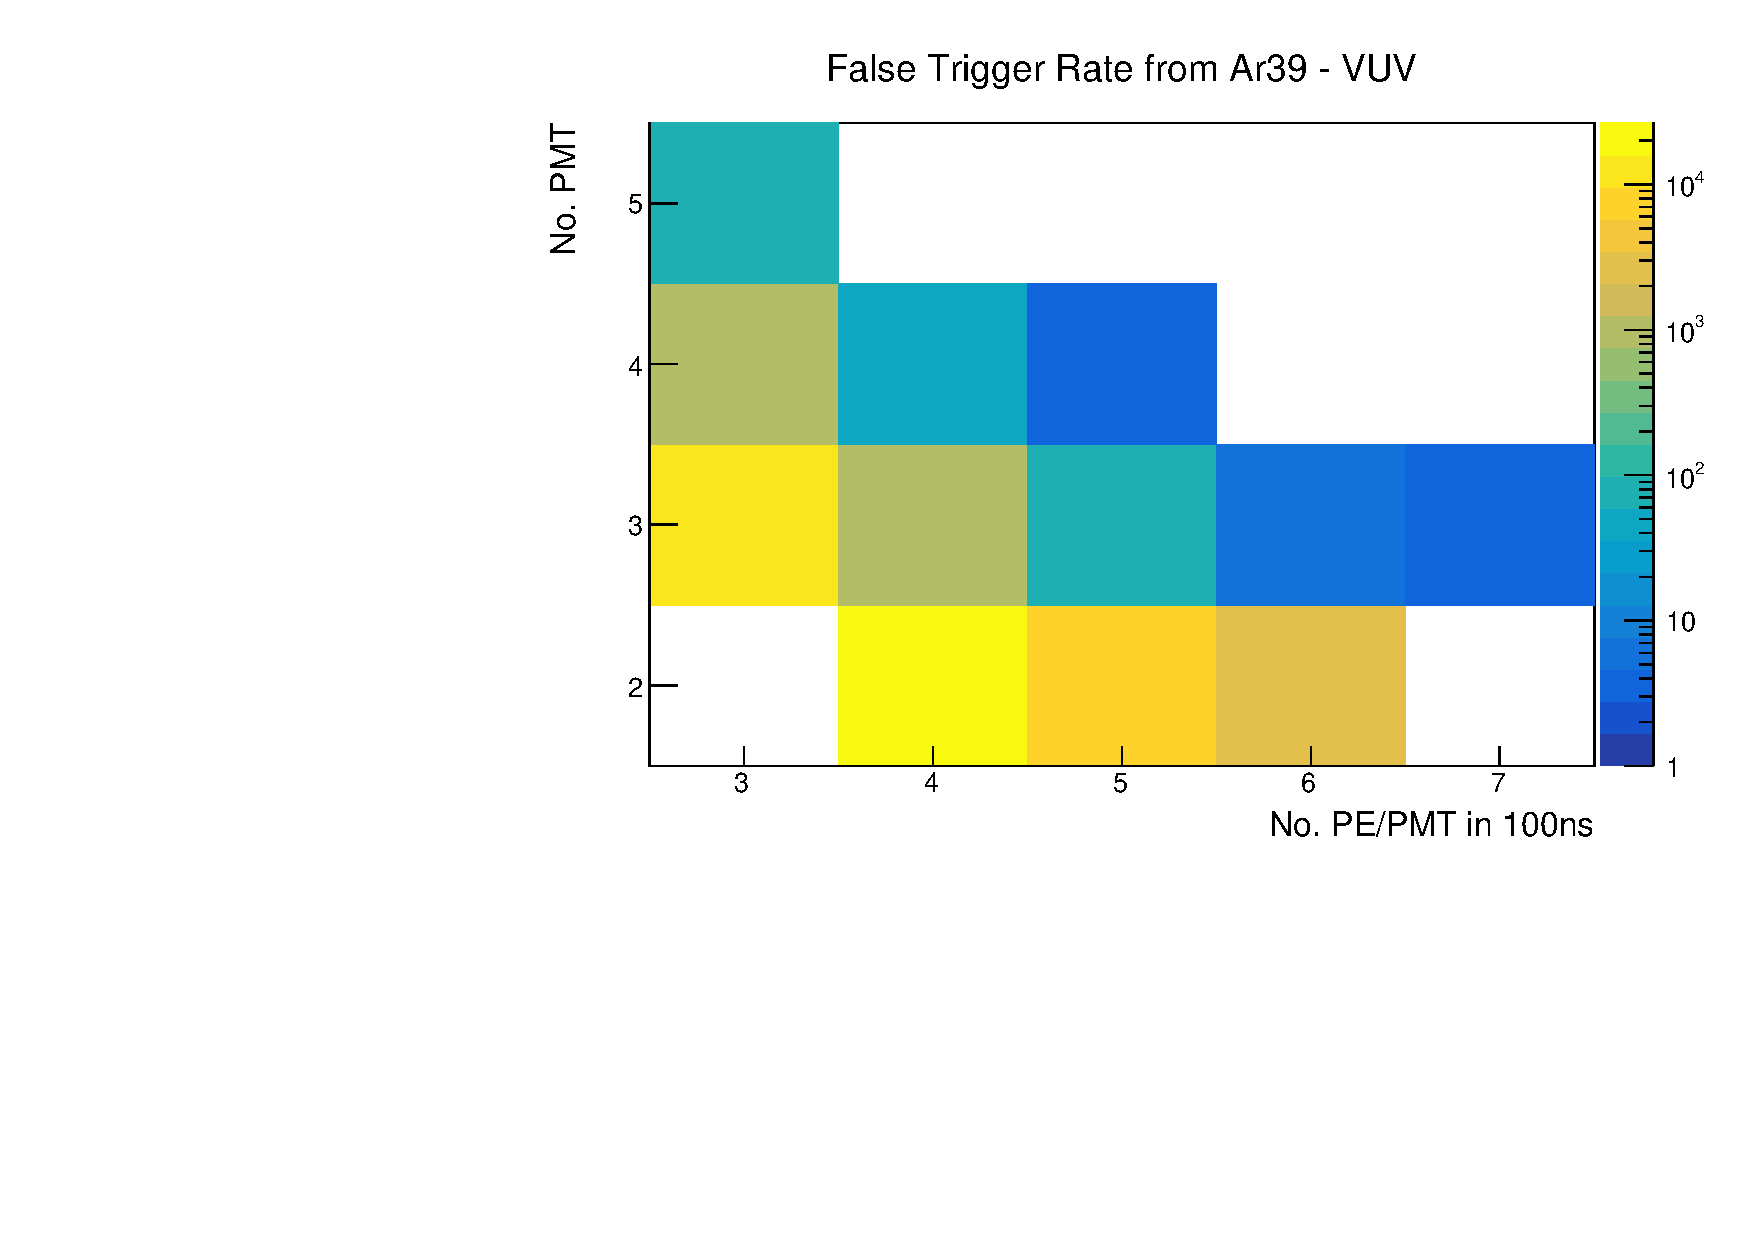
\includegraphics[width=0.43\textwidth]{trigger_map_100_vuv.pdf}
      \caption{Comparison of effective cuts to reduce $^{39}$Ar trigger rate for different LDS configuraitons. Time between PMTs seeing signal increased from 10 to 100 ns. The colour indicates the rate of triggers, and as such should be minimised. Therefore in this case, the most effective cuts are identified by the bins with the lowest value (most blue). Note that the plots are not normalised to one another.}\label{ar39_cut_maps_100ns}
\end{figure}

Figure \ref{10vs100} takes the 3 PMT cut for both 10 and 100 nanoseconds to compare how increasing the PEs removes the background. The 100 nanosecond case (dashed) is always greater than the respective 10 nanosecond case (solid), aside from a threshold of 7 for the full foils configuration. These values are within 0.0185 Hz of each other and is within any expected error.

\begin{figure}[H]
\center
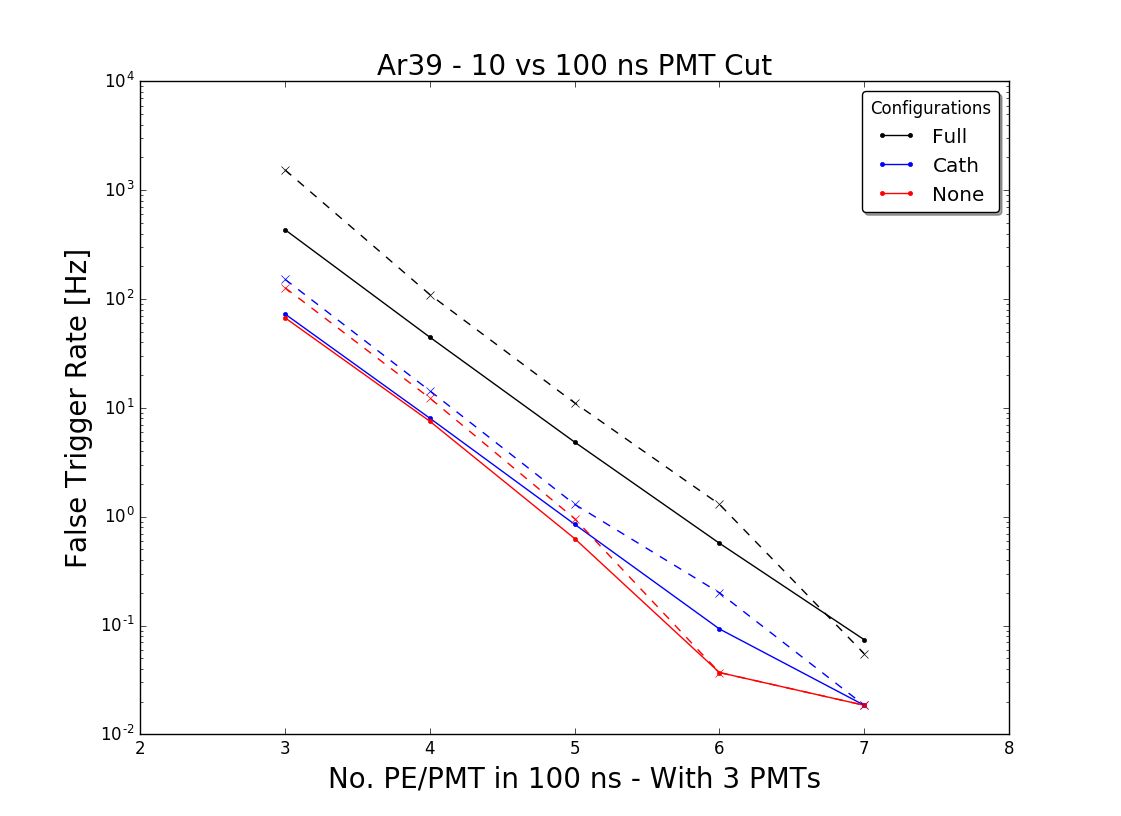
\includegraphics[width=0.5\textwidth]{ar39_10v100.png}
\caption{False trigger rate from $^{39}$Ar given three different LDS configurations, where solid lines indicate a 10 nanosecond cut on 3 PMTs, while the dashed line has a time window of 100 nanoseconds.}\label{10vs100}
\end{figure}

The second consideration when selecting the trigger threshold is to configure the threshold such that the supernova $\nu$ signal efficiency is kept as high as reasonably possible. For the same cuts demonstrated in Figure \ref{ar39_cut_maps}, the \% losses of supernova events are shown in Figure \ref{sn_cut_maps}.

\begin{figure}[H]
  \center
      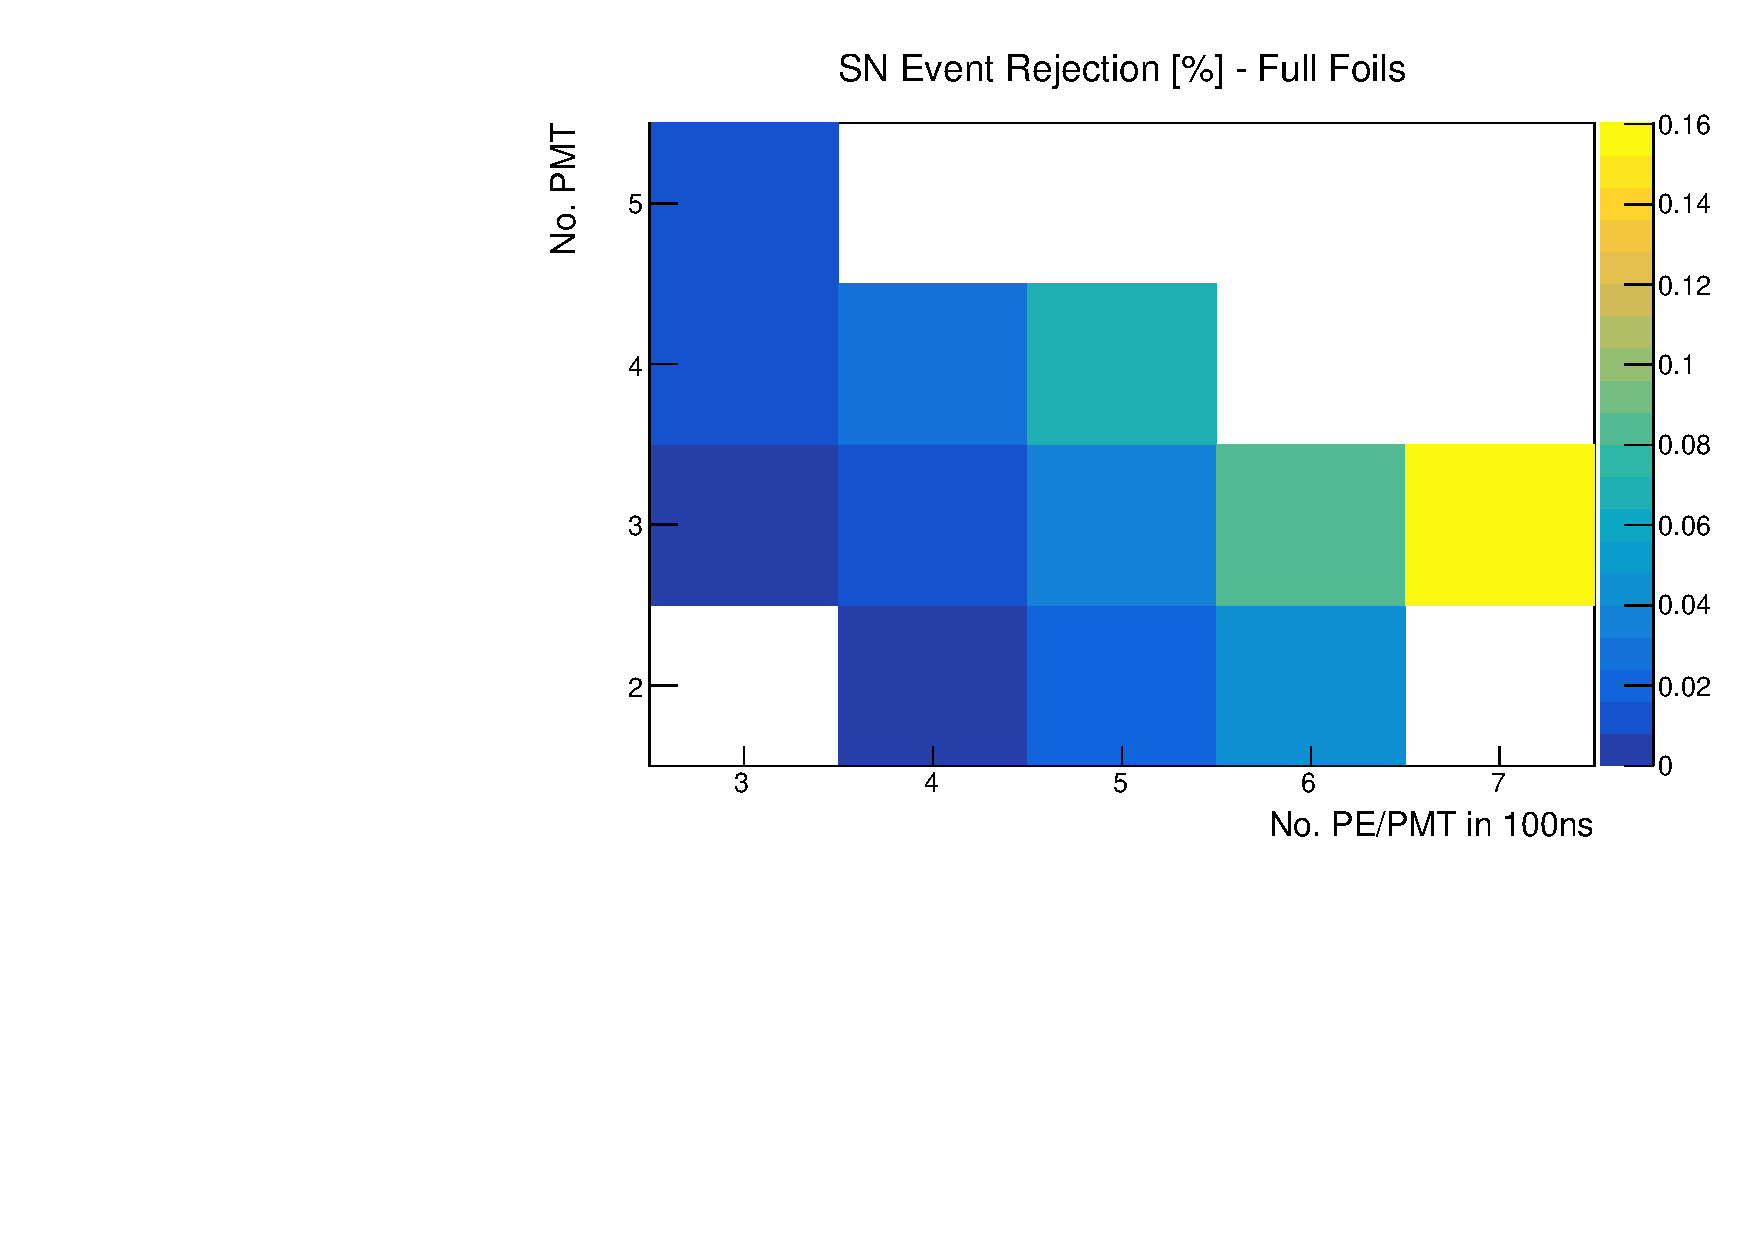
\includegraphics[width=0.43\textwidth]{sn_trigger_map_fullfoils.pdf}
      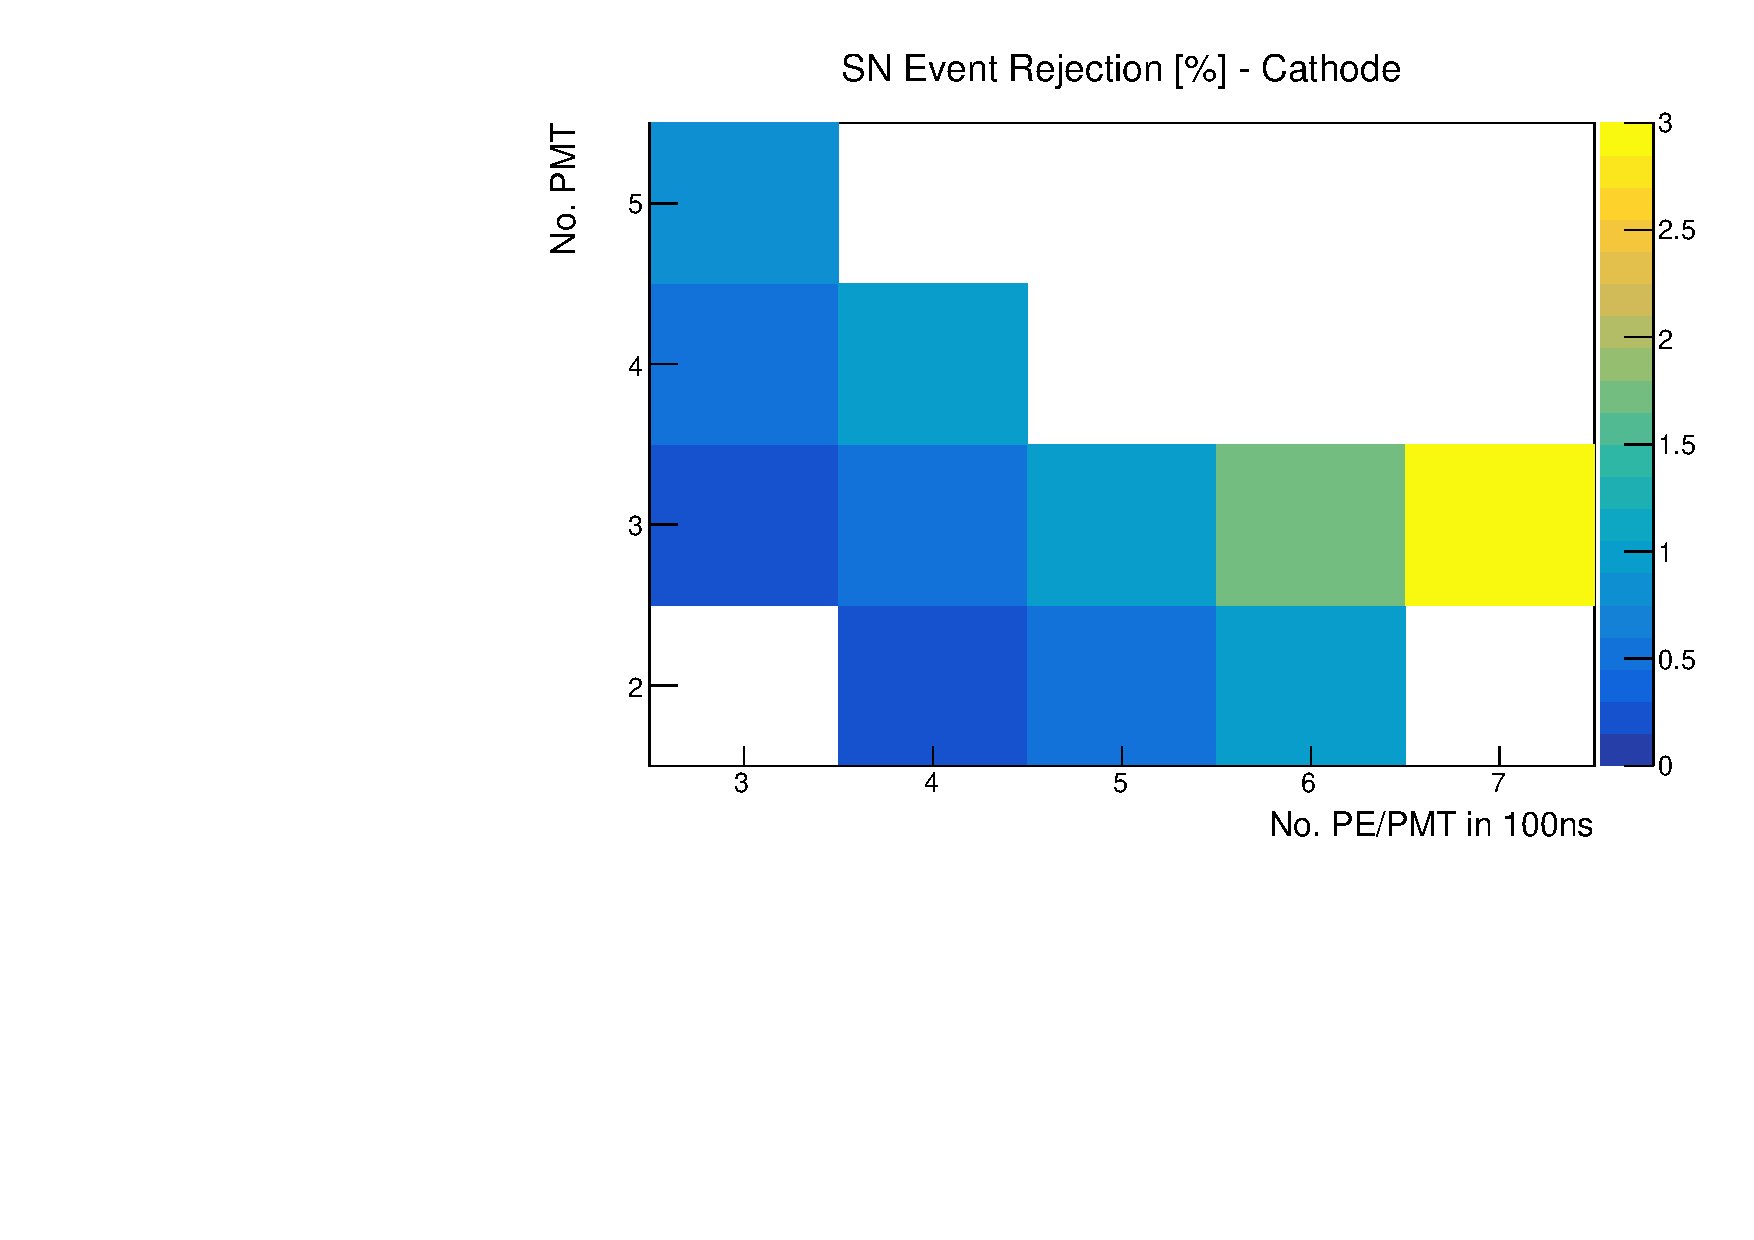
\includegraphics[width=0.43\textwidth]{sn_trigger_map_cathode.pdf}
      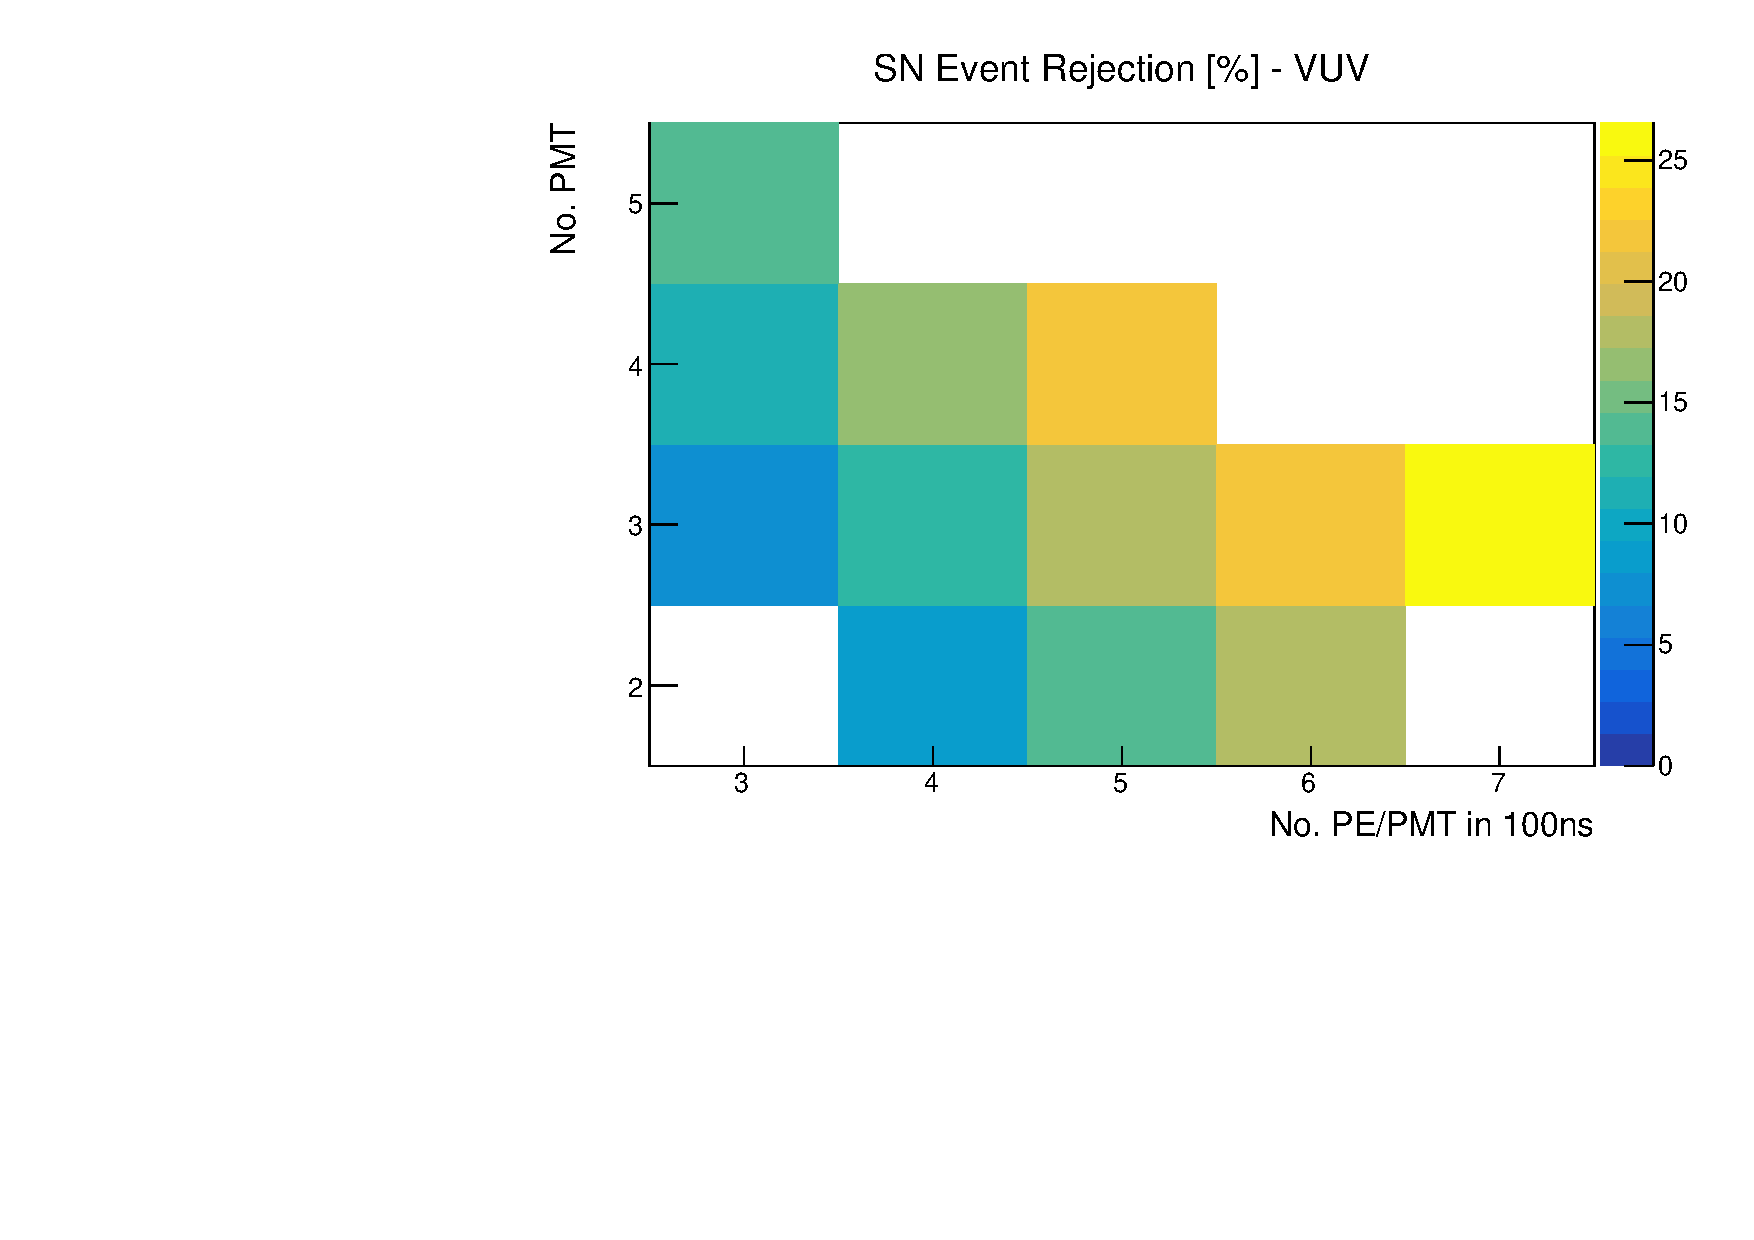
\includegraphics[width=0.43\textwidth]{sn_trigger_map_vuv.pdf}
      \caption{Comparison of thresholds on supernova detection efficiency for different LDS configurations. Colour indicates 1 - Efficiency, and as such should be minimised. Therefore in this case, the most effective cuts are identified by the bins with the lowest value (most blue). Note that the plots are not normalised to one another.}\label{sn_cut_maps}
\end{figure}

The results from Figure \ref{sn_cut_maps} echo results from before, where increasing the threshold or number of PMTs required to trigger begins rejecting supernova events along with the $^{39}$Ar. As the plots are not normalised across the different LDS configurations, it is therefore worth noting how little an impact changing thresholds have on the supernova signal given the full foils case - which sees maximum losses of around 0.16\%. Comparatively the cathode case has a maximum loss of around 4\% and the VUV case up to 27\%. Considering the 3 PMT case, a comparison between the full foils, cathode foils, and no foils case for the supernova efficiency  can be made in Figure \ref{sn_efficiency}. 

\begin{figure}[H]
\center
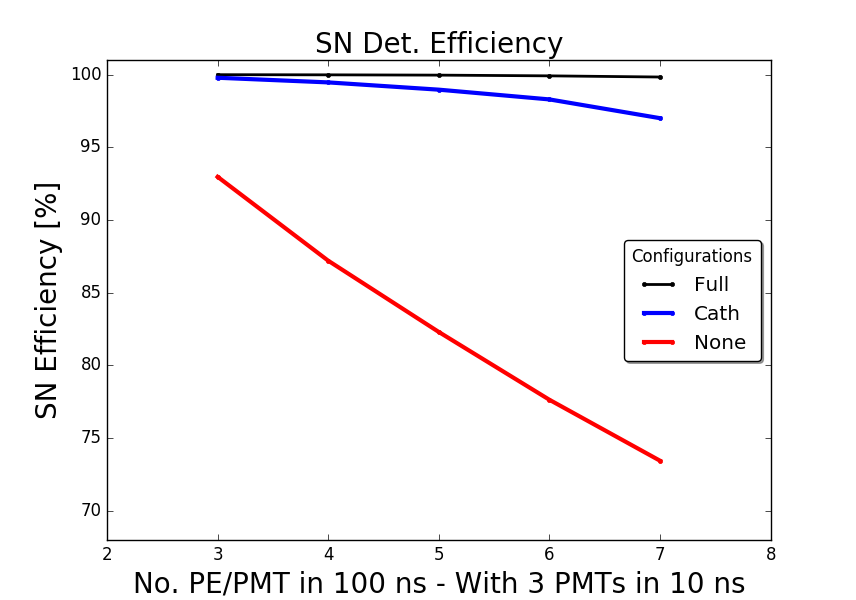
\includegraphics[width=0.5\textwidth]{updated_efficiency_labels.png}
\caption{Efficiency of threshold detecting photoelectrons produced from a supernova neutrino event as a function of the number of photoelectrons required on a PMT, given a 3 PMT case. The error bars are purely statistical.}\label{sn_efficiency}
\end{figure}

Much like in the single event case, the higher light yield systems perform better in terms of efficiency, despite having a higher background photon rate. The cathode and full foil configuration efficiencies remains above 90\% even for higher cuts, while the efficiency dips for the no foil case. This is due to the lack of uniformity in the LDS, such that events produced further from the photocathode have very few photons detected. 

Considering both results from the $^{39}$Ar study and the supernova study, it clearly displays that the cuts oppositely impact the desirable outcome. Assuming that equal weight can be given to the supernova efficiency, and rejecting the $^{39}$Ar background, then the sets of Figures \ref{ar39_cut_maps} and \ref{sn_cut_maps} can be considered together to find the optimal bin for minimising the background and maximising the signal.

%By taking the $^{39}$Ar trigger rate and dividing it by the \% efficiency of detecting supernova neutrinos, this gives a single value, when minimised indicates low background trigger rate and high efficiency. The results shown in Figure \ref{combo_cut_maps} visualise the combined considerations of both minimising the background and maximising signal efficiency, where bins with lower values have a low trigger rate, high efficiency, or both.

%\begin{figure}[H]
%\center
%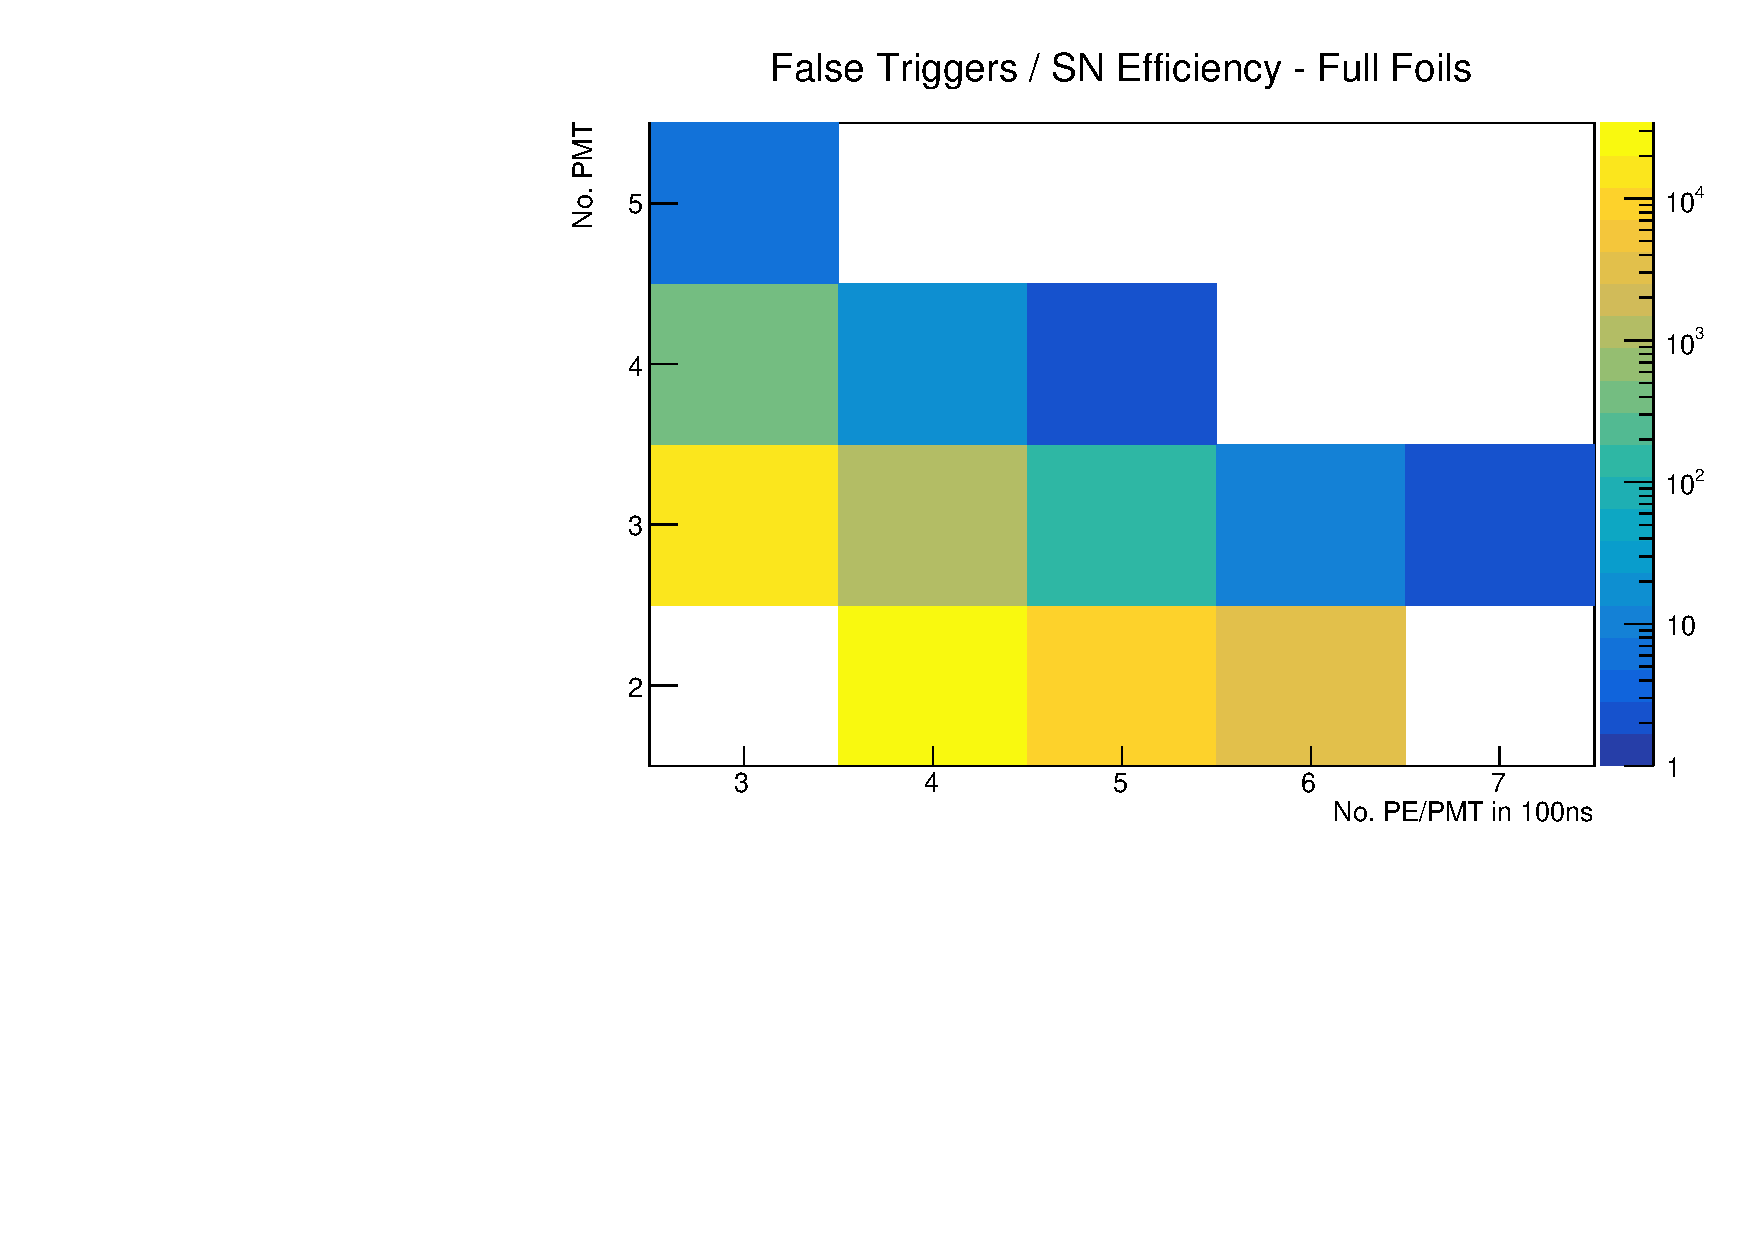
\includegraphics[width=0.43\textwidth]{trig_vs_efficiency_fullfoils.pdf}
%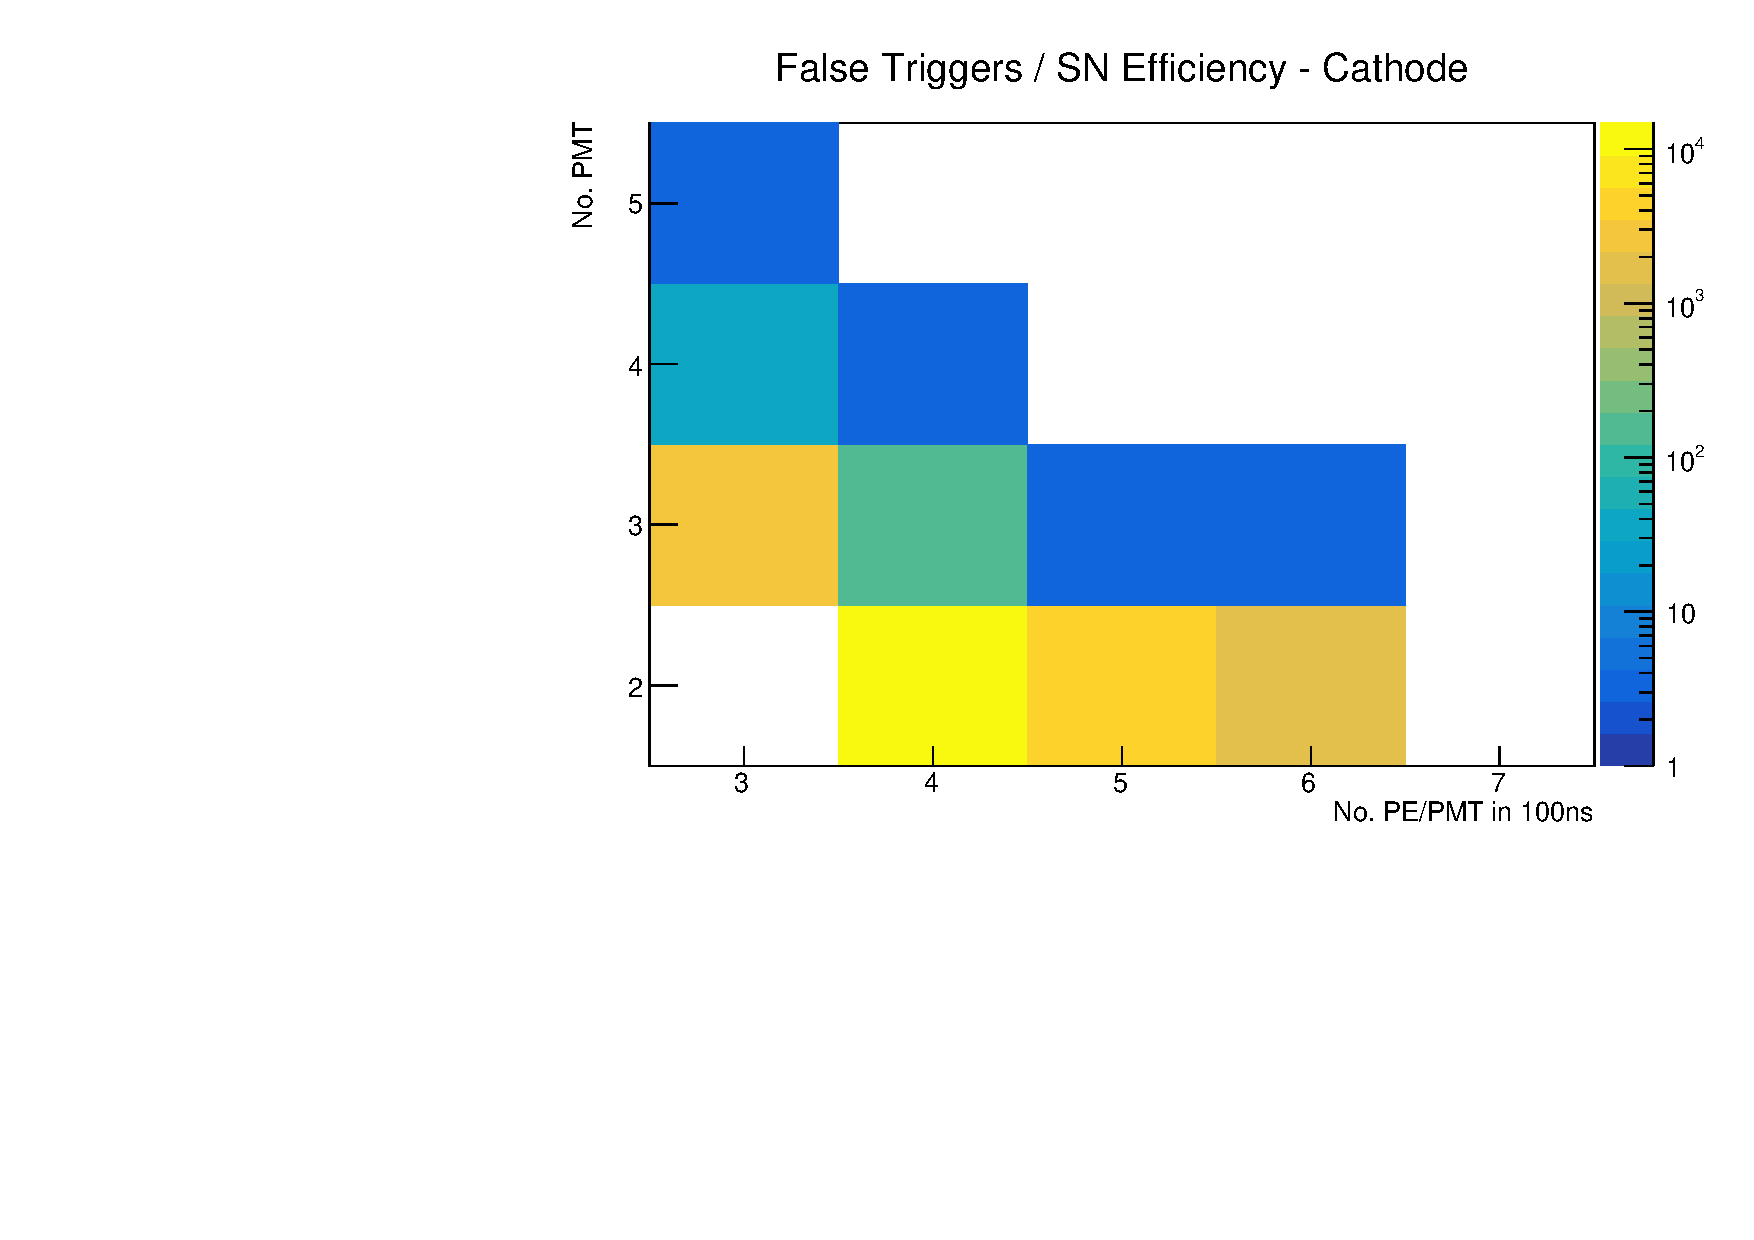
\includegraphics[width=0.43\textwidth]{trig_vs_efficiency_cathode.pdf}
%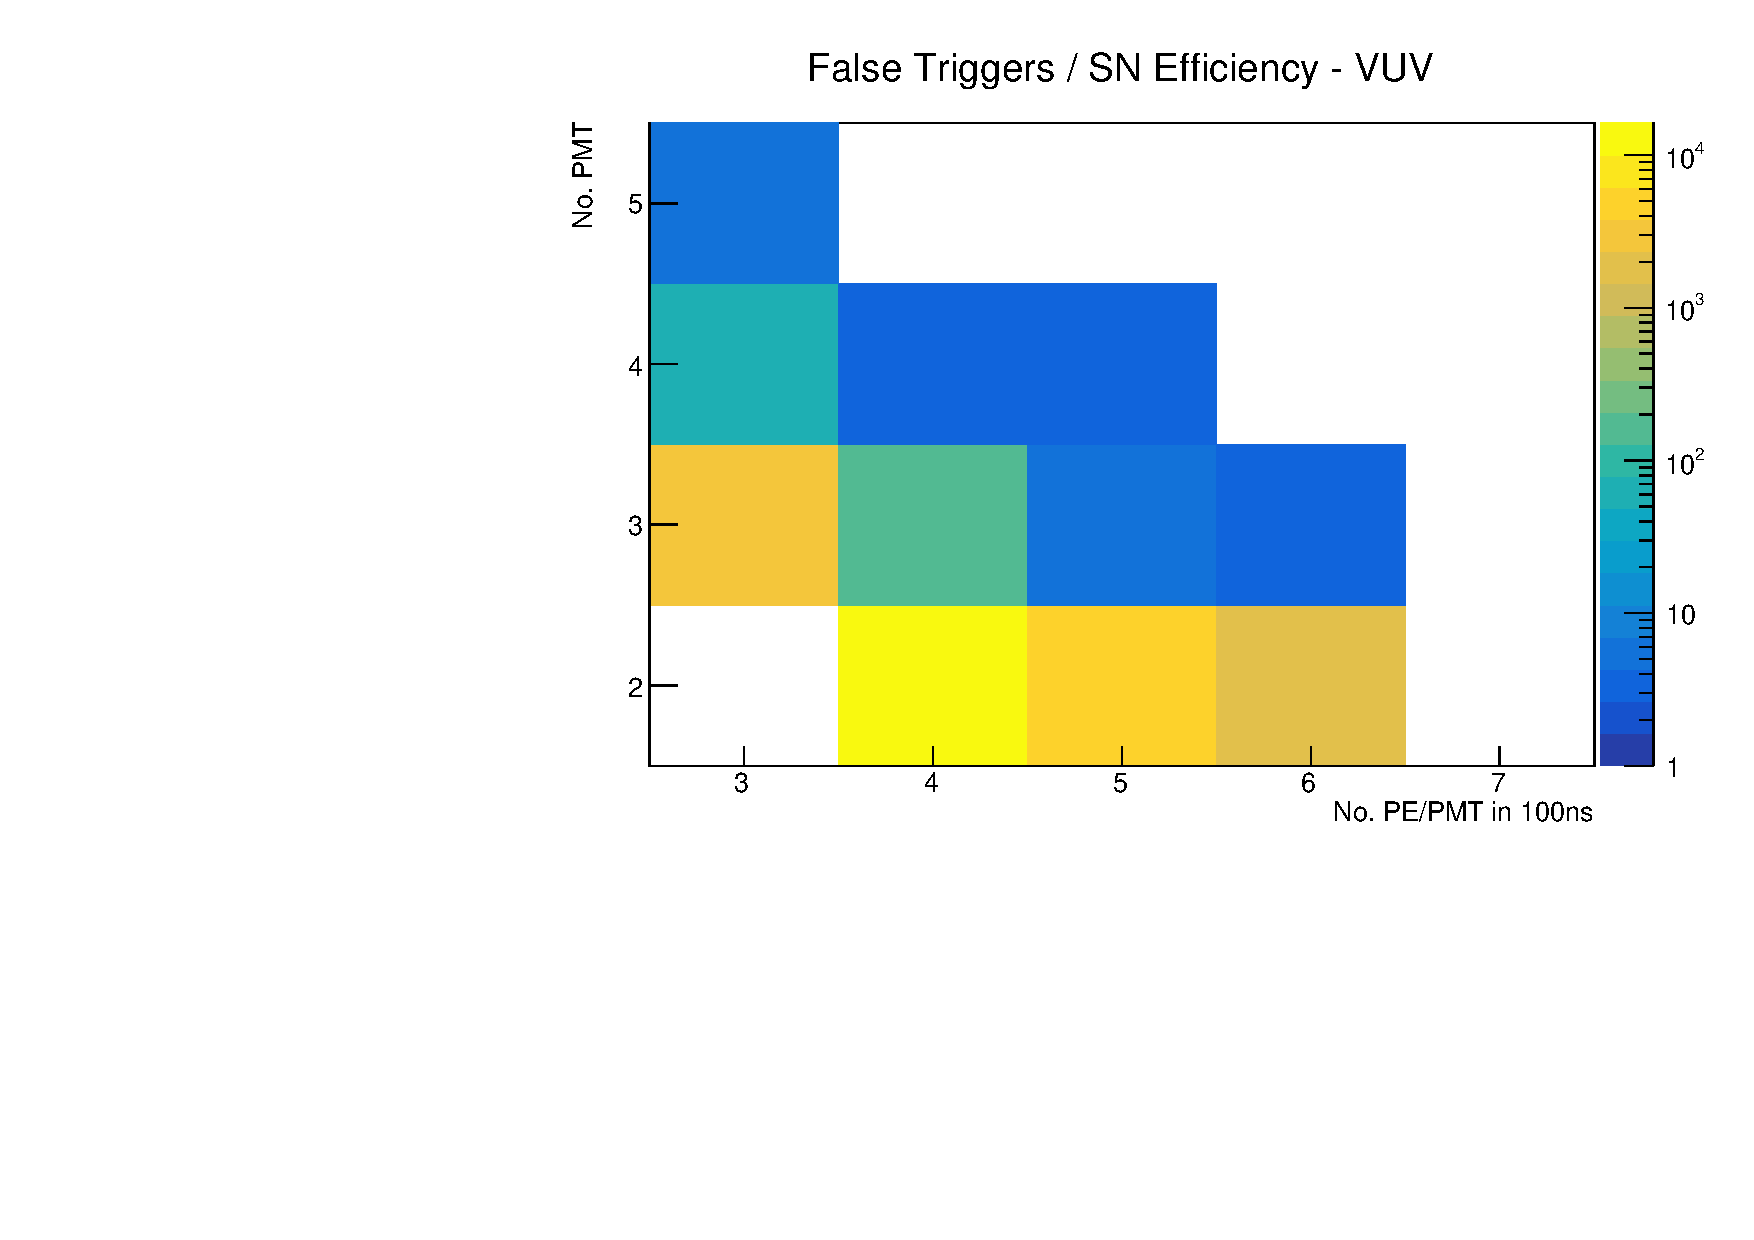
\includegraphics[width=0.43\textwidth]{trig_vs_efficiency_vuv.pdf}
%\caption{Comparison of cuts for the $^{39}$Ar trigger rate divided by the \% supernova neutrino detection efficiency given three different LDS configurations. The colour indicates the intensity of the bin, where the lowest value bin is best (most blue). A more blue bin means that either the $^{39}$Ar trigger rate is low, the \% supernova efficiency is very high, or both.}\label{combo_cut_maps}
%\end{figure}

Results are shown on a single plot for the 3 PMT case where the detection efficiency for supernova $\nu$ and the inverse of the trigger rate (average time between triggers) are shown in Figure \ref{efficiency_trigger_twinaxis}, where the solid line is for the left axis and the dashed line the right axis. The colour scheme is as before with black being the full foils configuration, blue cathode foils, and red no foils. As was shown in the previous plots, when increasing the cuts both the supernova $\nu$ detection efficiency decreases and the average time between triggers increases.

\begin{figure}[H]
\center
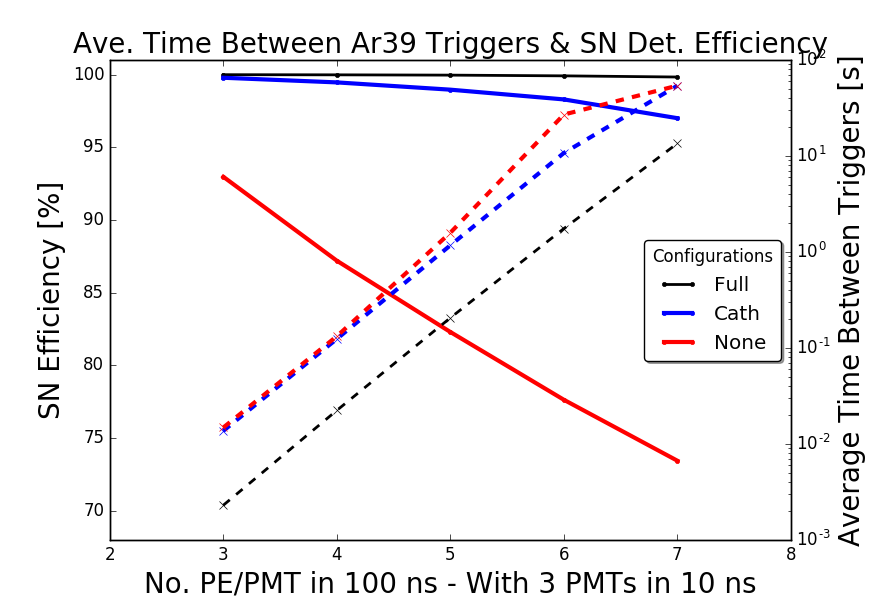
\includegraphics[width=0.5\textwidth]{updated_efficiency_purity_labels.png}
\caption{For the 3 PMT case, the supernova $\nu$ trigger efficiency (solid lines) and the time between triggers (dashed lines) are displayed simultaneously with their respective trends for increasing the number of photoelectrons per PMT needed to trigger.}\label{efficiency_trigger_twinaxis}
\end{figure}

As the supernova efficiency for events in the full foils configuration is consistently better than 99\% even at the highest thresholds, this configuration provides several values where the background triggers are nearly zero. This is similar to the cathode configuration, where losses in efficiency are rather small - up to 3\%. Comparatively the VUV only case, where the losses in efficiency are much higher than cases where reflective foils are included, up to 27\%. Despite this, the most effective thresholds are the highest, as this effectively reduces the background signal to zero, with minimum efficiency across all configurations at 73\%. The 7 PE/PMT see the lowest background, with 5 PMT and 3  PE/PMT performing only slightly worse. As no preference is assigned to either rejecting background or signal efficiency this topic should be given more discussion in the future.

%%%%%%%%%%%%%%%%%%%%%%%%%%%%%%%%%%%%%%%%%%%%%%%%%%%%%%%%%%
%%%%%%%%%%%%%%%%%%%%%%%%%%%%%%%%%%%%%%%%%%%%%%%%%%%%%%%%%%

\section{Conclusion}\label{ar39_conclusion}

Taking a simple approach to simulating the response of the light system in SBND to $^{39}$Ar and supernova neutrinos: this study demonstrates the ability of the light system to reject $^{39}$Ar scintillation light with relatively simple cuts. Additionally, it displays physics results calculated with the use of the SBND optical simulation libraries.

The rate of false triggers compared to the efficiency of detecting supernova events raises the question of how suppressed the $^{39}$Ar signal needs to be to reasonably detect as many supernova neutrinos as possible. Even at an efficiency of 90\%, for only 10 supernova neutrino events inside the detector, 1 is missed. In this discussion one of the limitations of the study presents itself, in that other methods to differentiate between the signal and background are not considered, which may result in lower thresholds.  The responses of the light system nor how these cuts should be directly implemented in concert with other possible scintillation backgrounds are not considered. Results from the Light Simulation Technote \cite{light_sim_technote} show how the VUV and not the visible component is most often responsible for saturating the PMTs, leading to the conclusion that the VUV component will also be most compact for triggering. However the additional light signal from visible light are what contribute to both $^{39}$Ar and supernova neutrino events reaching the trigger threshold value.

In an idealised system where the system electronics and DAQ are not involved, the conclusion remains that $^{39}$Ar should not be a problem for detection of low energy events using the light system, despite the large number of decays per second, provided some steps are taken to mitigate its influence. The ability to implement a trigger suggested here is still under investigation, as well as other background sources which could play a key role in the thresholds set for the light system. At the moment, it is believed that a trigger could be constructed such that when the system triggers, it enters a state of continuous readout, despite individual PMT threshold levels. Nonetheless, the most desirable trigger configuration from the simulated suggestions, are those which involve the lowest individual PMT thresholds, but also the lowest $^{39}$Ar background. This corresponds to trigger configurations which have a large number of PMTs involved, but a small individual threshold, to increase the possible energy resolution.

The fast optical libraries generated for simulating light system responses in SBND enabled this simple study of how a constant background of low energy ionising events create a constant background for the light system, which could interfere with acquisition of important events, such as supernova neutrinos. Despite these backgrounds having a high frequency compared to supernova neutrino events, employing simple cuts based on the arrival times of photons can isolate the supernova neutrino events with high efficiency. However, if the complete rejection of the background signals is a priority, for the no reflective foil system, the supernova neutrino detection efficiency drops below 80\%. Whereas the higher light yield configurations, where some reflective foils are implemented, see significantly better efficiency. Nonetheless, the simulations demonstrate the usefulness of the fast optical library and how a simple approach could be sufficient in SBND to suppress constant backgrounds for the light system.

%%%%%%%%%%%%%%%%%%%%%%%%%%%%%%%%%%%%%%%%%%%%%%%%%%%%%%%%%%
%%%%%%%%%%%%%%%%%%%%%%%%%%%%%%%%%%%%%%%%%%%%%%%%%%%%%%%%%%

%\section{Scintillation Signals of Ionic Recombination}
%
%As with the $^{39}$Ar, the concern for low energy event detection is that background scintillation sources can reduce efficiency and purity. This section again makes use of the fast optical library to consider effects from a potential other source.
%
%\subsection{Concept and Motivation}
%
%Inside an ionization detector, when charge passes through the medium, pairs of electrons and ions are generated. The electrons which do not recombine are drifted to the anode, while the positive ions drift to the cathode. However it is not well investigated what kind of interaction the ion undergoes when it reaches the cathode. Currently the MicroBooNE experiment is seeing an optical rate considerably higher than expected and are considering possible explanations. One hypothesis is that when these ions reach the cathode, they undergo recombination with the electrons in the cathode, and in doing so, emit scintillation light. In the case of off-beam measurements, this would come from cosmic interactions within the detector. The origin of these higher rates are under investigation.
%
%The following sections outline how these ions have been simulated using the fast optical libraries and how they could modify the conclusions reached above regarding supernova neutrino detection and cuts on $^{39}$Ar background.
%
%\subsection{Simulation Method}
%
%The first step is to estimate the amount of energy being deposited into the detector by the ionising cosmic rays. A rough estimation of the cosmic rate to be 100 $\mu$/s/m$^{2}$ is used. Assuming all of the cosmic particles are MIPs, they deposit 2 MeV/cm and travel 2.5 m through the detector. Using these estimated values, the cosmic flux on SBND deposits around $10^{6}$ MeV/s. In order to generate an electron-ion pair for argon 23.6 eV are needed, and roughly 30\% of the ions created actually drift at a field value of 500 V/cm. Lastly, assuming that all ions reach the cathode regardless of production location and produce one photon when recombining, the number of photons generated per second is about $10^{10}$.
%
% Based on this theory, all of the scintillation light from the ions recombining should originate from voxels on the cathode. For the fast optical simulation in SBND there are 8000 voxels lining the cathode of one TPC, where one of these voxels is randomly selected for the ion's recombination. For technical reasons, it is more efficient to produce a larger number of photons per voxel, rather than select a new voxel per photon. But due to the large number of photons being generated per second, the simulation can still loop over the cathode voxels enough to avoid undersampling.
%
%The produced photons are then ``propagated'' to the PMTs by applying the visibility. This average rate recorded by all PMTs depends on the light yield of the system, shown in Table \ref{ions_table}. The rate is extremely large compared to the number of photons generated due to $^{39}$Ar or supernova neutrinos. However, assuming the cosmic flux is constant, each photon's arrival time was assigned randomly in time, rather than propagated through the detector. This was motivated by the large number of events in a given time washing out any discernible structure due to scintillation or transport time.
%
%\begin{table}[H]
%\center
%	\begin{tabular}{| c || c | c |}
%	\hline
%	Configuration & Rate - Total [MHz] & No. Photoelectron Per PMT per 100 ns \\
%	\hline
%	 & &\\
%	Full Foils & 300 & 0.5 \\
%	 & &\\
%	Cathode & 140 & 0.2\\
%	 & &\\
%	No Foils & 8 & 0.02\\
%	\hline
%	\end{tabular}
%\caption{Simulated rate from scintillation light generated by positive ions recombining on the cathode for three different light system configurations.}\label{ions_table}
%\end{table}
%
%\subsection{Simulation Results}
%
%The ions recombining on the cathode generate a considerable floor of light, characteristically different from scintillation light generated by $^{39}$Ar, in arrival time distributions and magnitude. It is expected that the cuts developed for the $^{39}$Ar will need to be modified when the signals from both backgrounds are combined. At the lower photoelectron cuts the rate should be higher than the only $^{39}$Ar case, however increases in the threshold should still remove a considerable rate. This can be explained by the random timing of the scintillation light, which does not mimic a single supernova neutrino event, but rather arrives uniformly throughout time. With the cut increased to a sufficient level, the combined background can be removed for all configurations of the light system. Figure \ref{} shows the performance of the various cuts and Figure \ref{ions_false_trigger} the performance when considering only the 3 PMT cuts.
%
%\begin{figure}[H]
%\center
%\includegraphics[width=0.5\textwidth]{updated_ions_trigger_vs_cut.pdf}
%\caption{Rate of triggers due to the combined $^{39}$Ar and theorized ions recombining on the cathode versus the number of photoelectrons required per PMT to trigger. The three different configurations are shown.}\label{ions_false_trigger}
%\end{figure}
%
%**Supernova ion studies go here**
%
%\subsection{Conclusion - Ionic Scintillation}
%
%The signal generated by the ions recombining on the cathode is considerable, and noticeable when requiring lower levels of thresholds on the PMTs. Without some kind of trigger in place, the light system would likely to be overwhelmed. However at more reasonable values of thresholds, above 5 photoelectrons per PMT, the contribution from the ions is small. As the cuts are constructed with coincidences in mind, the random scintillation light produced at the cathode likely does not regularly have enough frequency to reach multiple PMTs. Considering the cuts have to be modified very little with the introduction of the ion scintillation light, the efficiencies for supernova neutrino detection remain valid, if not conservative, as the ion signal would slightly enhance the probability for a low energy neutrino to pass the cut.
%
%One of the limitations of the study comes from the estimation of the cosmic flux and its composition. The simulation assumes simply that the flux is composed of muons and that the rate is approximately 100 $\mu$/m$^{2}$/s. However, for the purposes of reaching an estimate of the scintillation light produced by the ions as well as demonstrating the adaptability of the cuts applied to rejecting $^{39}$Ar, these limitations are not problematic.

%\section{Conclusion}
%
%The fast optical libraries generated for simulating light system responses in SBND enabled this simple study of how a constant background of low energy ionising events create a constant background for the light system, which could interfere with acquisition of important events, such as supernova neutrinos. Despite these backgrounds having a high frequency compared to supernova neutrino events, employing simple cuts based on the arrival times of photons can isolate the supernova neutrino events with high efficiency. However, if the complete rejection of the background signals is a priority, for the no reflective foil system, the supernova neutrino detection efficiency drops below 80\%. Whereas the higher light yield configurations, where some reflective foils are implemented, see significantly better efficiency. Nonetheless, the simulations demonstrate the usefulness of the fast optical library and how a simple approach could be sufficient in SBND to suppress constant backgrounds for the light system.

\begin{thebibliography}{1}

\bibitem{sn_spectrum} Irene Tamborra {\em et al.} {\em High-resolution supernova neutrino spectra represented by a simple fit}. Phys.Rev. D 86, 2012.

\bibitem{light_sim_technote} Diego Garcia-Gamez {\em et al.} {\em Light detection system simulations for SNBD}. SBND DocDB 1155, 2016.

\end{thebibliography}


%%%%%%%%%%%%%%%%%%%%%%%%%%%%%%%%%%%%%%%%%%%%%%%%%%%%%%%%%
%%%%%%%%%%%%%%%%%%%%%%%%%%%%%%%%%%%%%%%%%%%%%%%%%%%%%%%%%
\pagebreak
\appendix
\section{Alternate Binning Scheme for Single Events}\label{alt_binning}

As noted in Section \ref{limiting_bkg}, the PMTs at the centre of the plot are not joined together, rather due to the binning they appear as such. To keep the plots symmetry and reflect the rest of the PMT geometry as well as provide bins sufficiently large to discern colour the binning was selected as above. This section, however, provides an alternative binning scheme, which more accurately reflects the spacing of the PMTs, however suffers from having smaller bins.

\begin{figure}[H]
\center
\includegraphics[width=0.43\textwidth]{ar39_signal_map_rebin.pdf}
\includegraphics[width=0.43\textwidth]{sn_signal_map_rebin.pdf}
\includegraphics[width=0.43\textwidth]{sn_signal_map_higherE_rebin.pdf}
\caption{Comparison of single high-energy $^{39}$Ar, 5 MeV SN, and 22 MeV SN events in middle of detector using 60 PMTs. Single high-energy $^{39}$Ar expects about 50 hits, 5 MeV SN about 500 hits, and 22 MeV SN about 2400 hits. Shown are the results for the total light (VUV+visible) in the case of full reflective foils. Color (z-axis) corresponds to number of photoelectons.}\label{signal_maps_rebin}
\end{figure}

The rebinned histograms for the fast light case are also shown (Figure \ref{signal_maps_rebin_fastlight}).

\begin{figure}[H]
\center
\includegraphics[width=0.43\textwidth]{ar39_signal_map_rebin_fastlight_2.pdf}
\includegraphics[width=0.43\textwidth]{sn_signal_map_rebin_improved_fastlight.pdf}
\includegraphics[width=0.43\textwidth]{sn_signal_map_higherE_rebin_improved_fastlight.pdf}
\caption{Comparison of single high-energy $^{39}$Ar, 5 MeV SN, and 22 MeV SN events in middle of detector using 60 PMTs. Single high-energy $^{39}$Ar expects about 50 hits, 5 MeV SN about 500 hits, and 22 MeV SN about 2400 hits. Shown are the results for the total light (VUV+visible) in the case of full reflective foils. Color (z-axis) corresponds to number of photoelectons.}\label{signal_maps_rebin_fastlight}
\end{figure}

\end{document}
